% !TEX root = trkjet.tex

This section discusses the results from the previous section. 

%%cent dependence
The centrality dependence of \RDptr\ for two charged-particle \pt\ intervals: 1.0--1.6~\GeV\ and \mbox{6.3--10.0~\GeV}, and two different \ptjet\ ranges: 126--158 GeV and 200--251 GeV, is presented in Figure~\ref{fig:centdep}. The magnitude of these modifications decreases for more peripheral collisions and \RDptr\ approaches unity in 60--80\% central collisions for both \pt\ ranges, across the entire $ r < 0.8$ range under investigation. It can also be seen that the higher \ptjet\ range shows a larger modification in central collisions. 

\begin{figure}[h]
\centerline{
         \begin{tabular}{cc}
            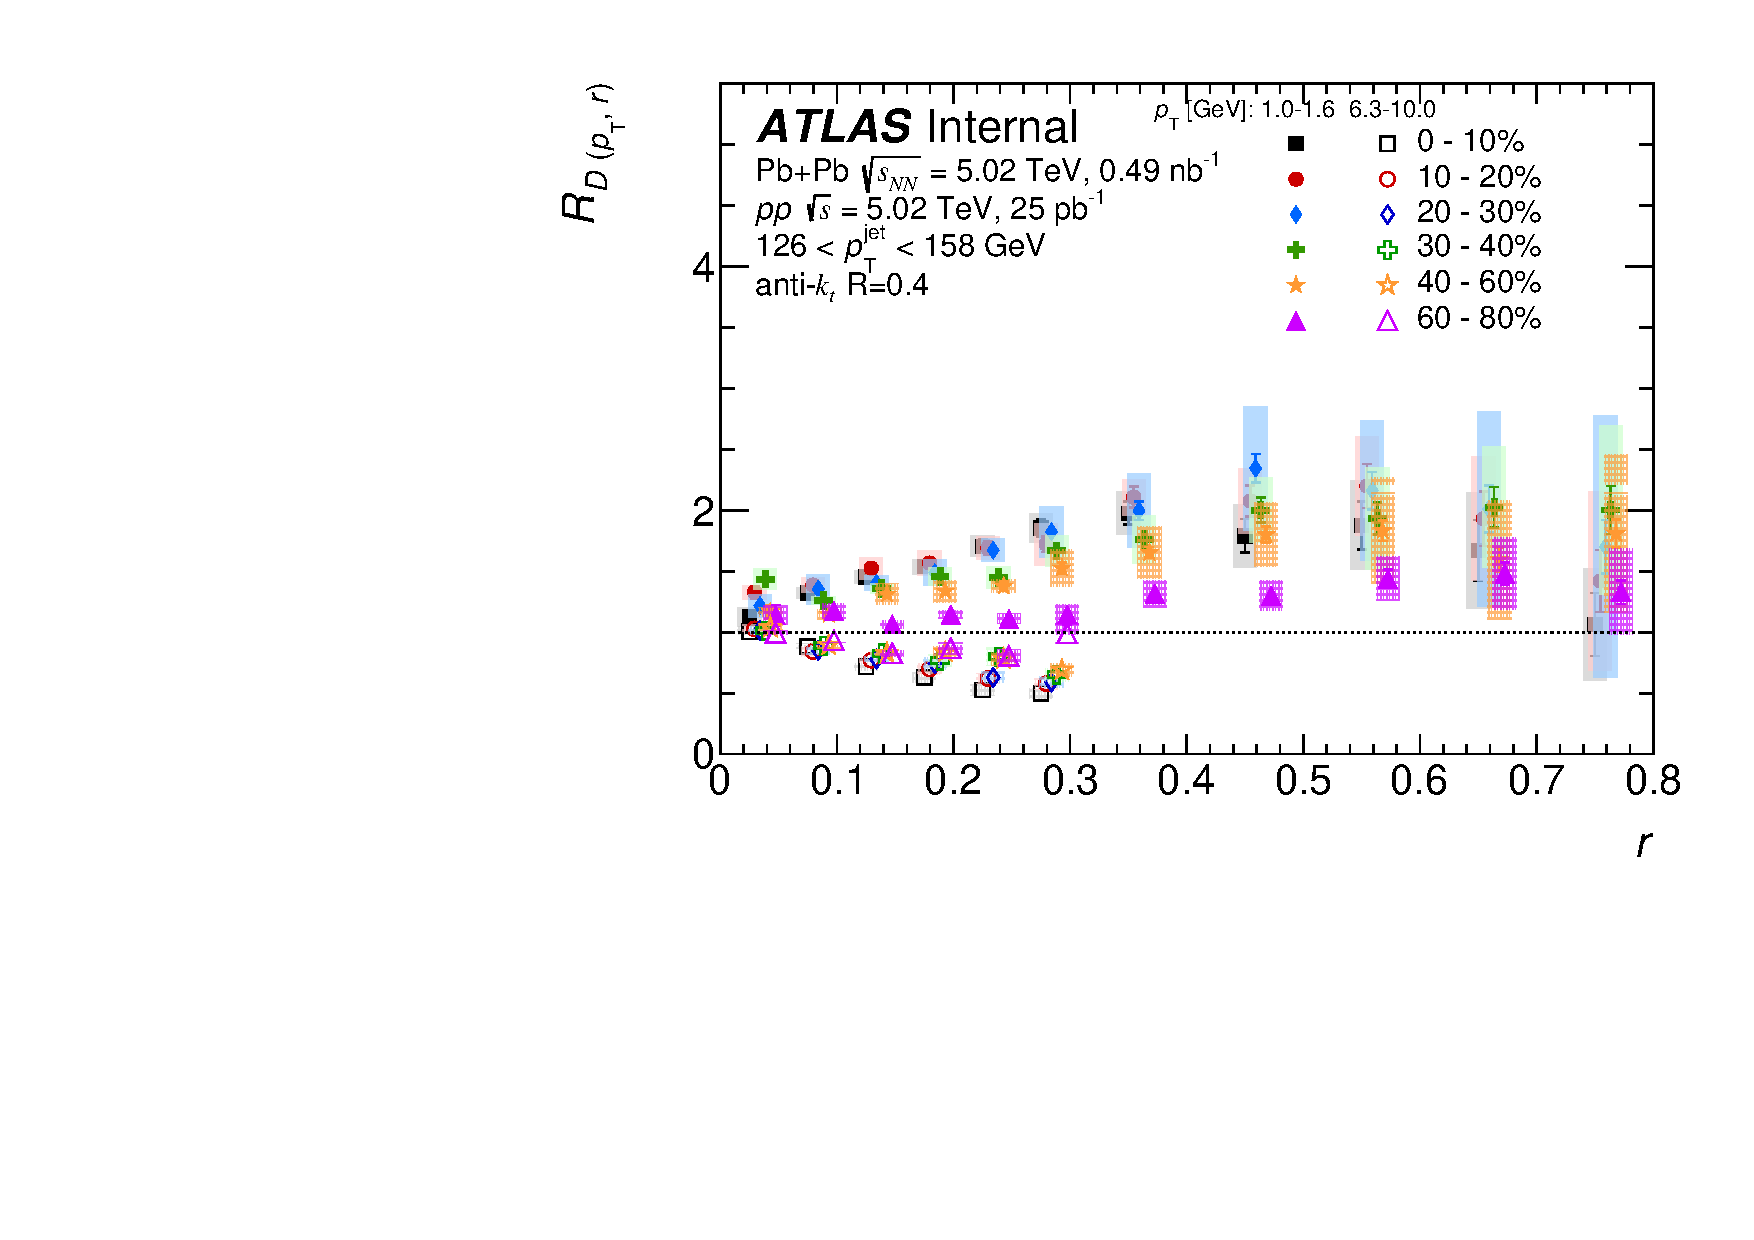
\includegraphics[width=0.5\textwidth]{figures/results/RDpT_dR_trk2_trk6_jet7.pdf} & 
            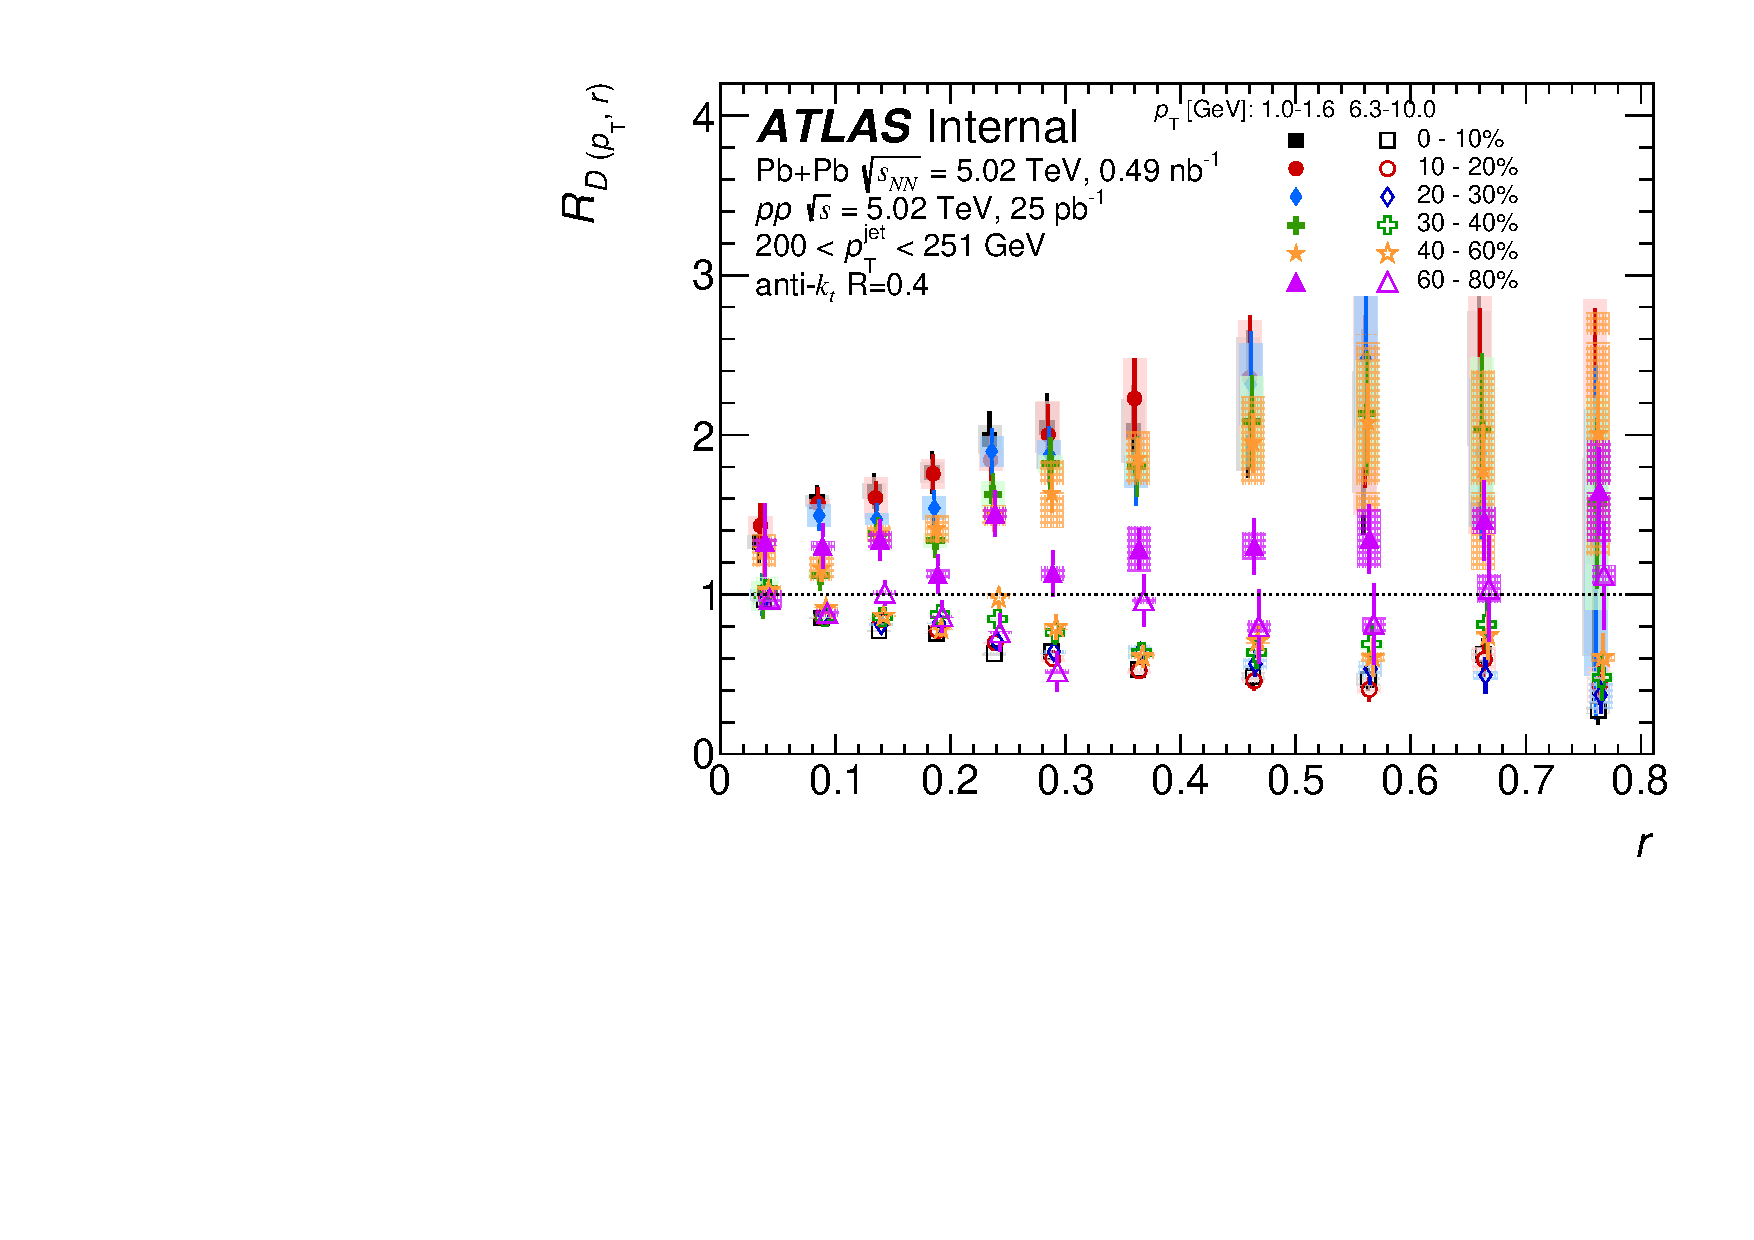
\includegraphics[width=0.5\textwidth]{figures/results/RDpT_dR_trk2_trk6_jet9.pdf} \\
      \end{tabular}
      }
\caption{The \RDptr\ distributions for \ptjet\ of 126--158~\GeV\ and 200--251~\GeV\ as a function of angular distance $r$ for two \pt\ selections and six centrality intervals (\pt\ selections are shown by closed and open symbols). The vertical bars on the data points indicate statistical uncertainties while the shaded boxes indicate systematic uncertainties. The widths of the boxes are not indicative of the bin size and the points are shifted horizontally for better visibility.}
\label{fig:centdep}
\end{figure}
%%%%%%%%%%%%%

%%pt jet dependence
The \ptjet\ dependence of \RDptr\ for two \pt intervals: 1.0--1.6~\GeV\ and \mbox{6.3--10.0~\GeV}, in 0--10\% central \pbpb\ collisions is presented in Figure~\ref{fig:ptjetdep}. A trend of increasing \RDptr\ with increasing \ptjet\ is observed for $0.0 < r < 0.25$ for low pt particles. The higher-\pt\ charged particles have \RDptr\ values that decrease with increasing \rvar; no significant dependence on \ptjet\ is observed. 

\begin{figure}[ht]
\centerline{
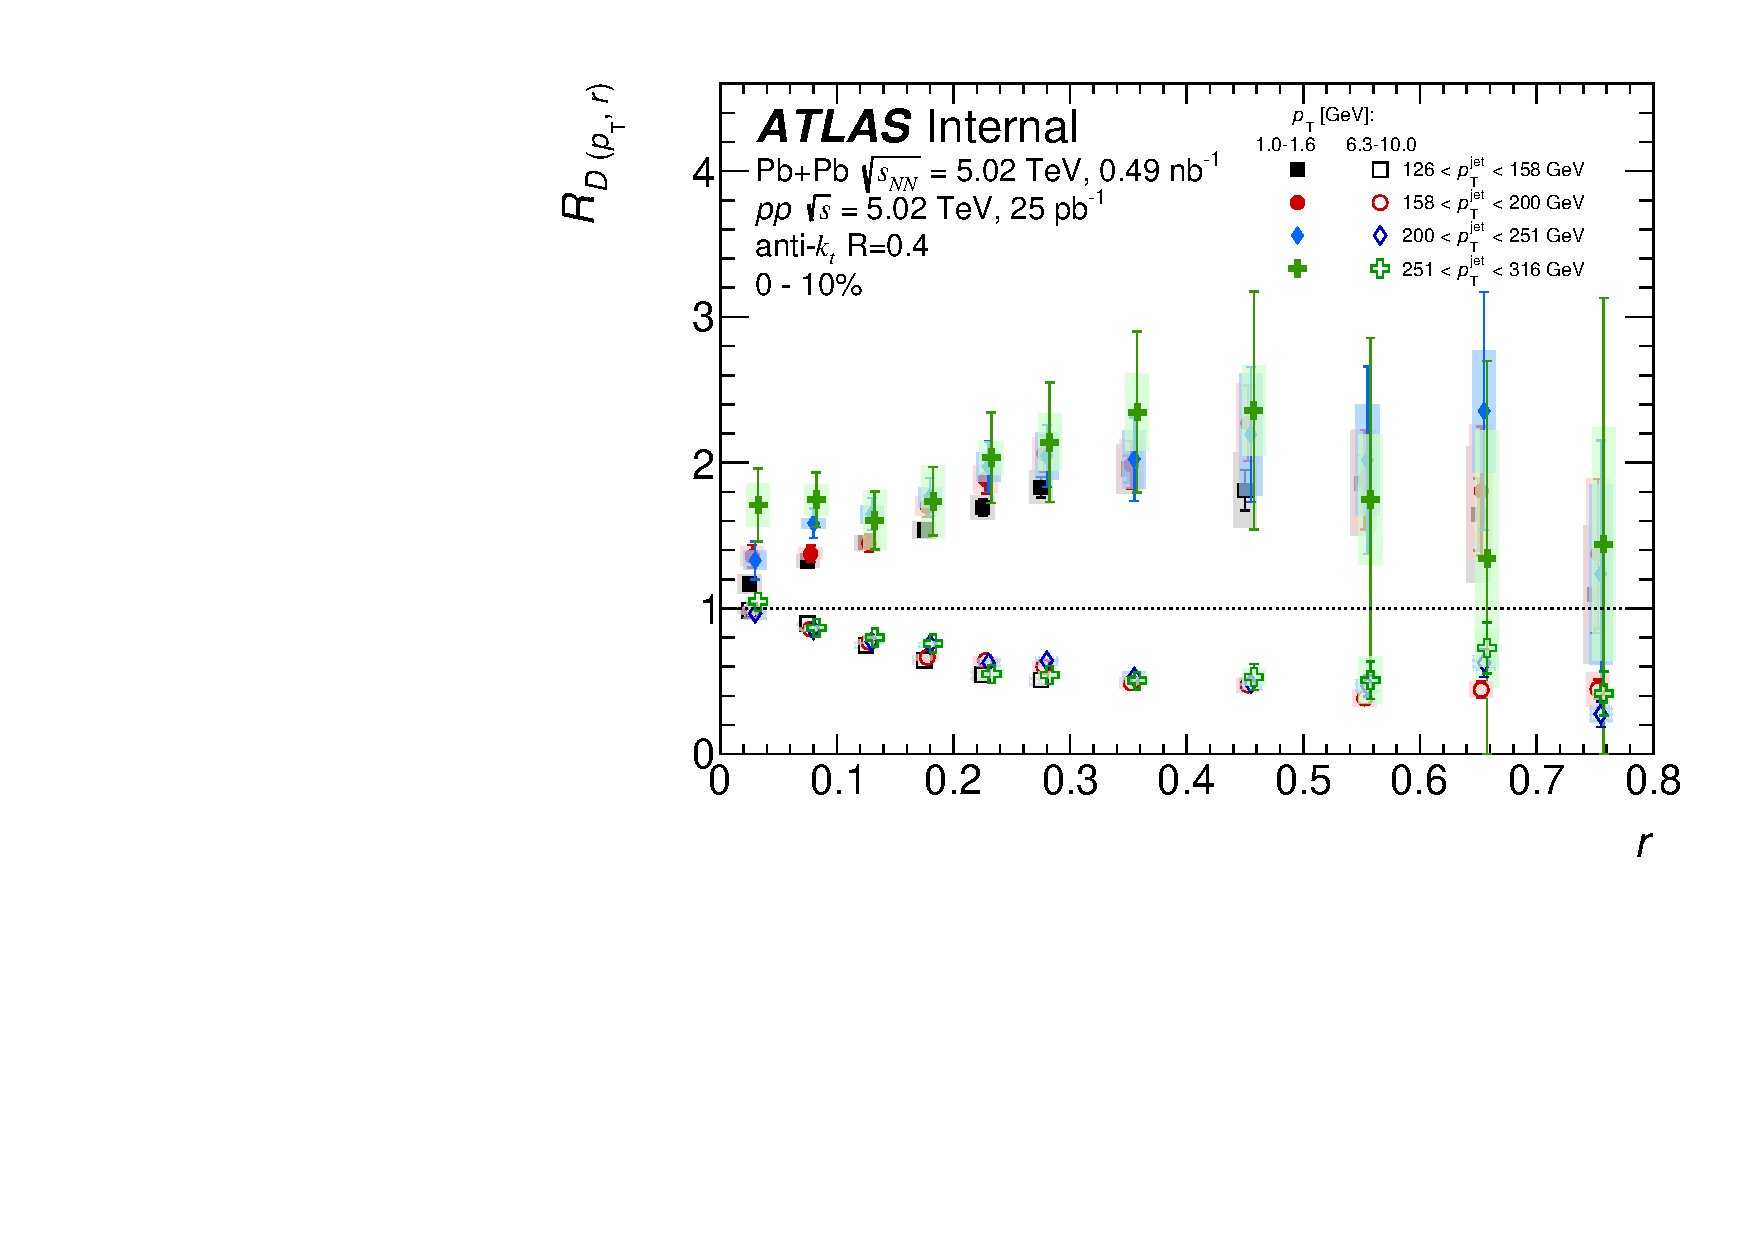
\includegraphics[width=0.8\textwidth]{figures/results/RDpT_dR_trk2_trk6_cent0.pdf} 
}
\caption{\RDptr\ as a function of \rvar\ for 0--10\% collisions for charged particles with 1.0~$< \pt <$~1.6~\GeV\
(closed symbols) and 6.3~$< \pt <$10.0~\GeV\ (open symbols) for different \ptjet\ selections. The vertical bars on the data points indicate statistical uncertainties while the shaded boxes indicate systematic uncertainties. The widths of the boxes are not indicative of the bin size and the points are shifted horizontally for better visibility.}
\label{fig:ptjetdep}
\end{figure}
%%%%%%%%%%%%%


%%pt track dependence
The charged particle \pt\ dependence of \RDptr\ for \mbox{$126 < \ptjet < 158$ GeV} and \mbox{$200 < \ptjet < 251$ GeV}, at a variety of angular distances from the jet axis in 0--10\% central and 60--80\% peripheral collisions is presented in Figure~\ref{fig:pttrkdep}. No suppression is observed for $r < 0.05$ across the entire \pt\ range under investigation. This can also be seen in Figure~\ref{fig:rdptr} and Figure~\ref{fig:rdptr_trk_cent}, where any suppression in the charged particle spectra is at distances larger than $r = 0.05 $from the jet axis. 

\begin{figure}
\centering{
\begin{tabular}{cc}
	 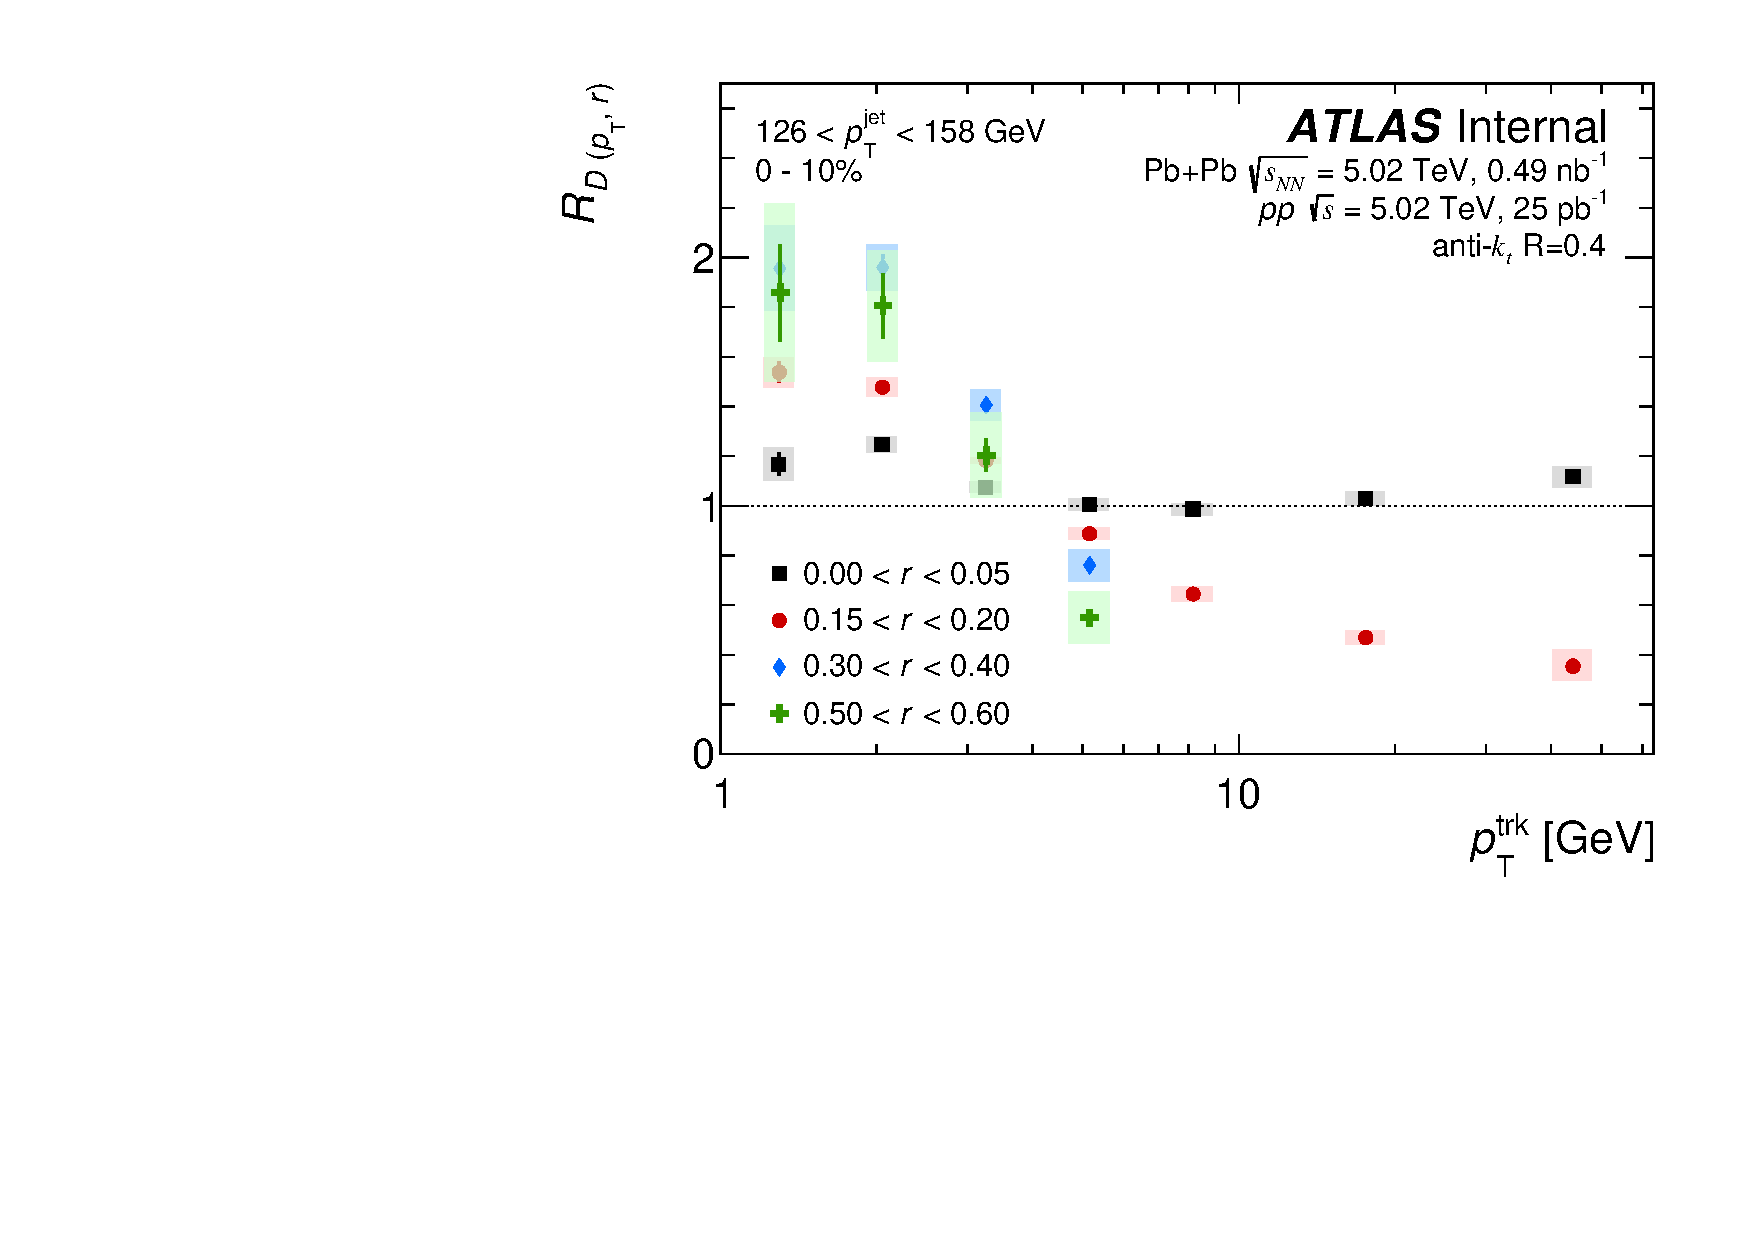
\includegraphics[width=0.5\textwidth]{results/RDpT_trkpt_jet7_cent0} &
	 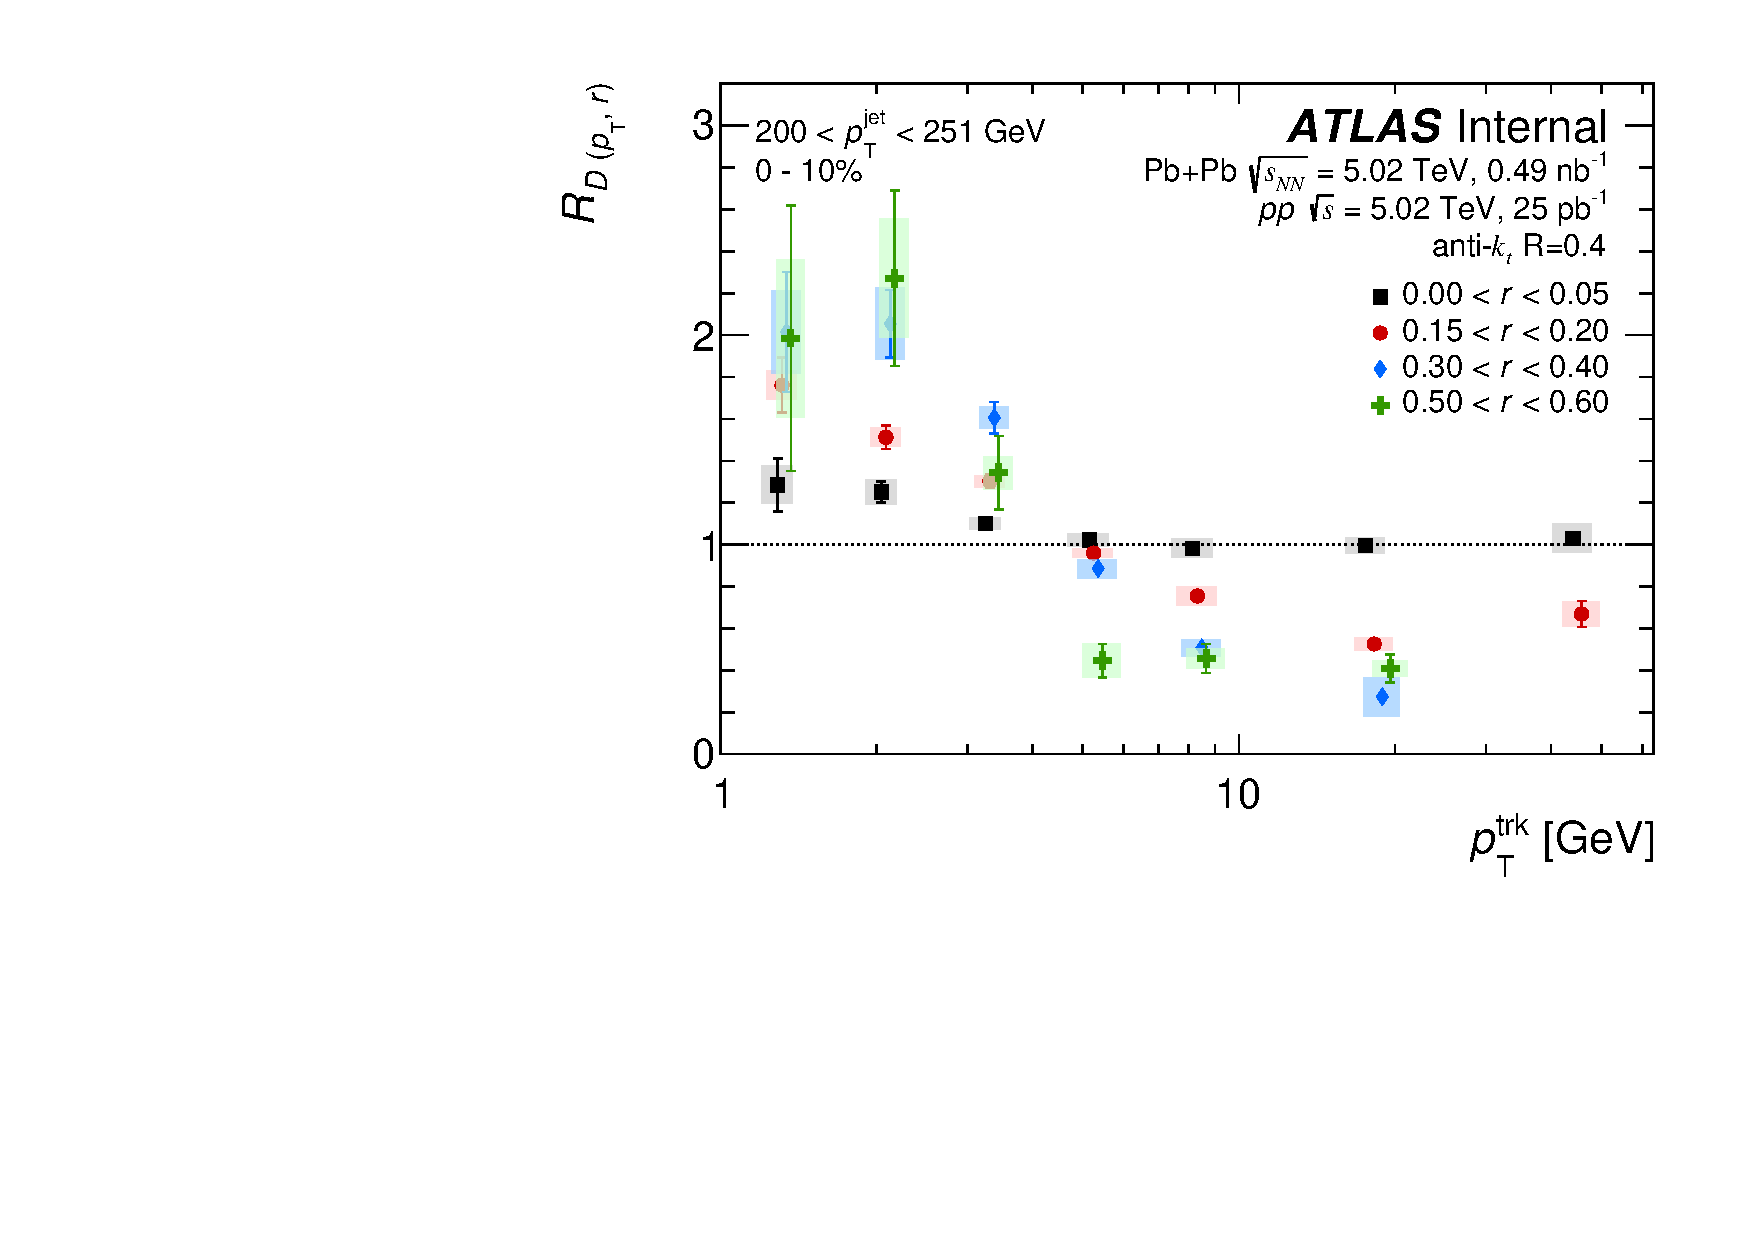
\includegraphics[width=0.5\textwidth]{results/RDpT_trkpt_jet9_cent0} \\
	 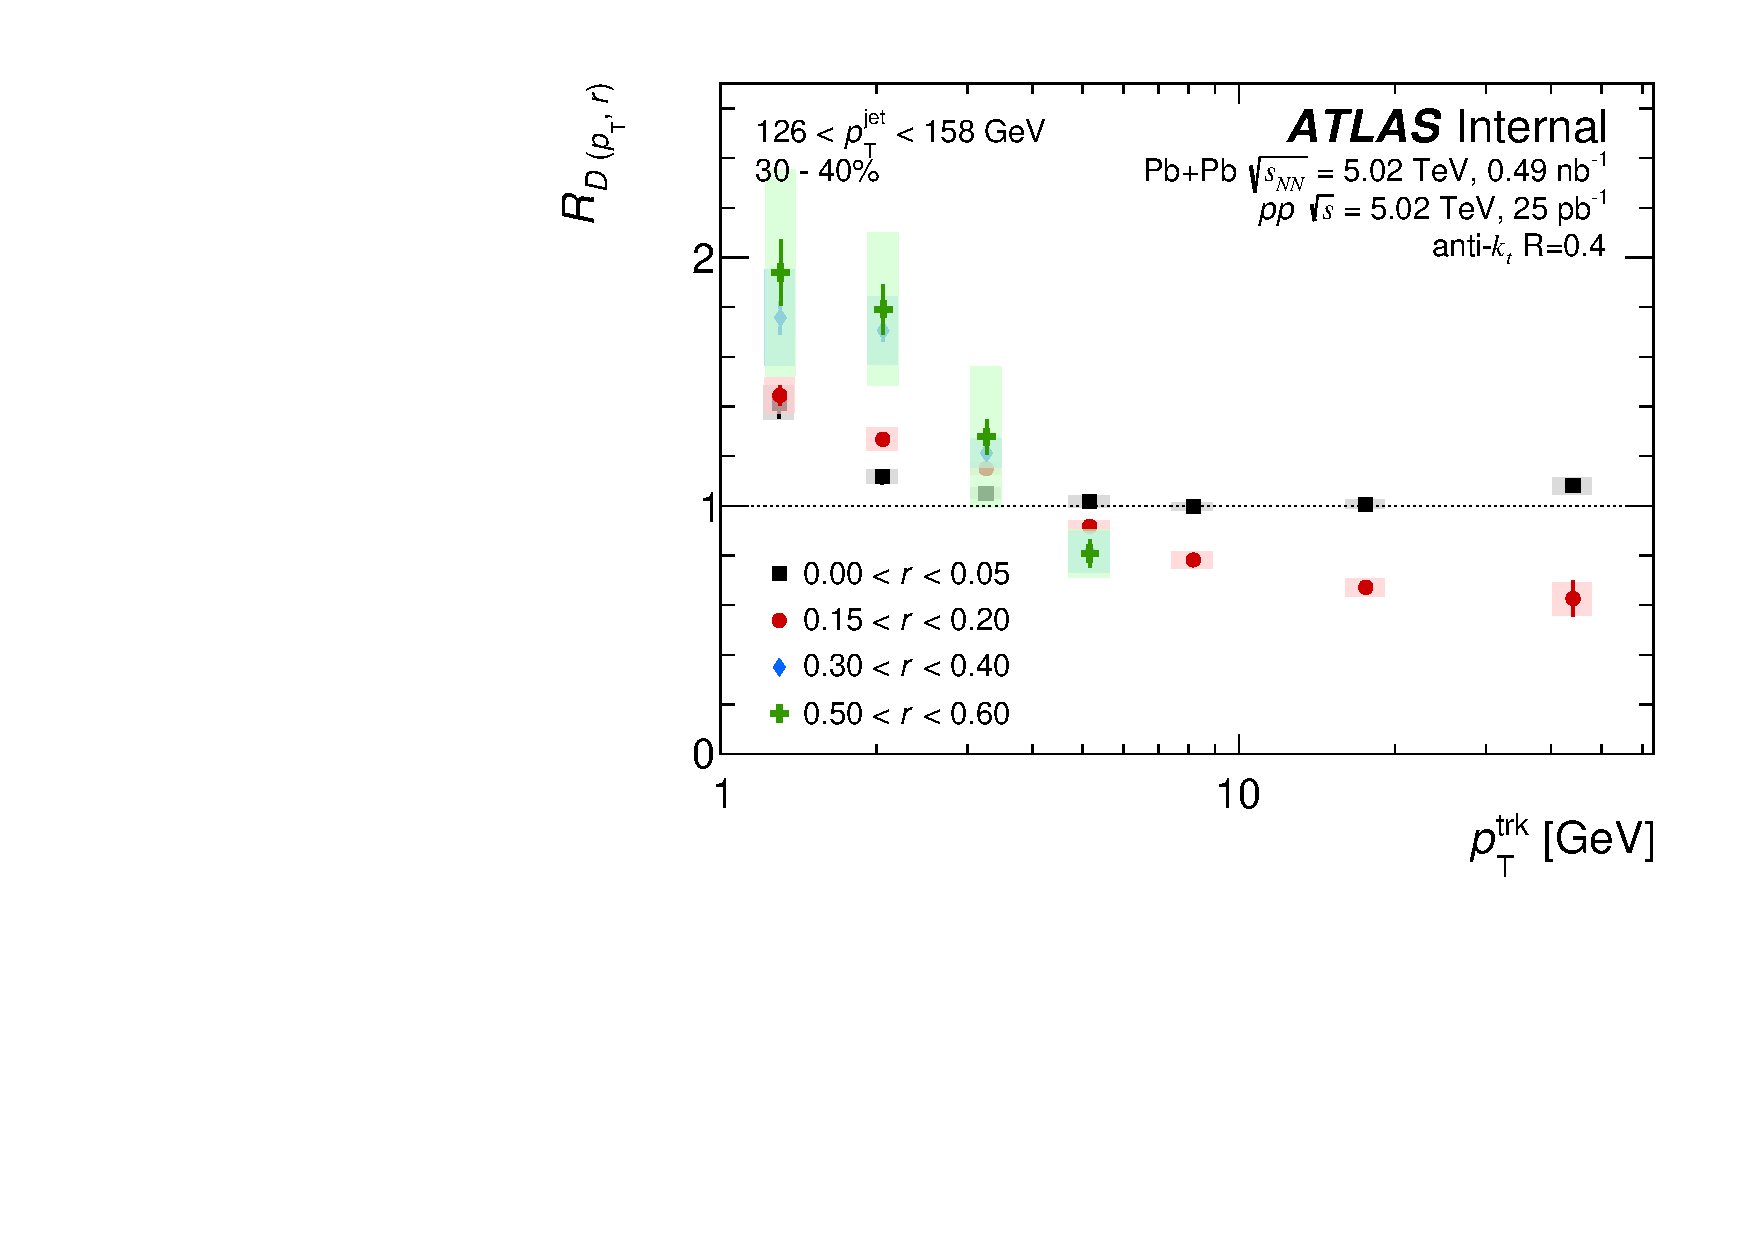
\includegraphics[width=0.5\textwidth]{results/RDpT_trkpt_jet7_cent3} &
	 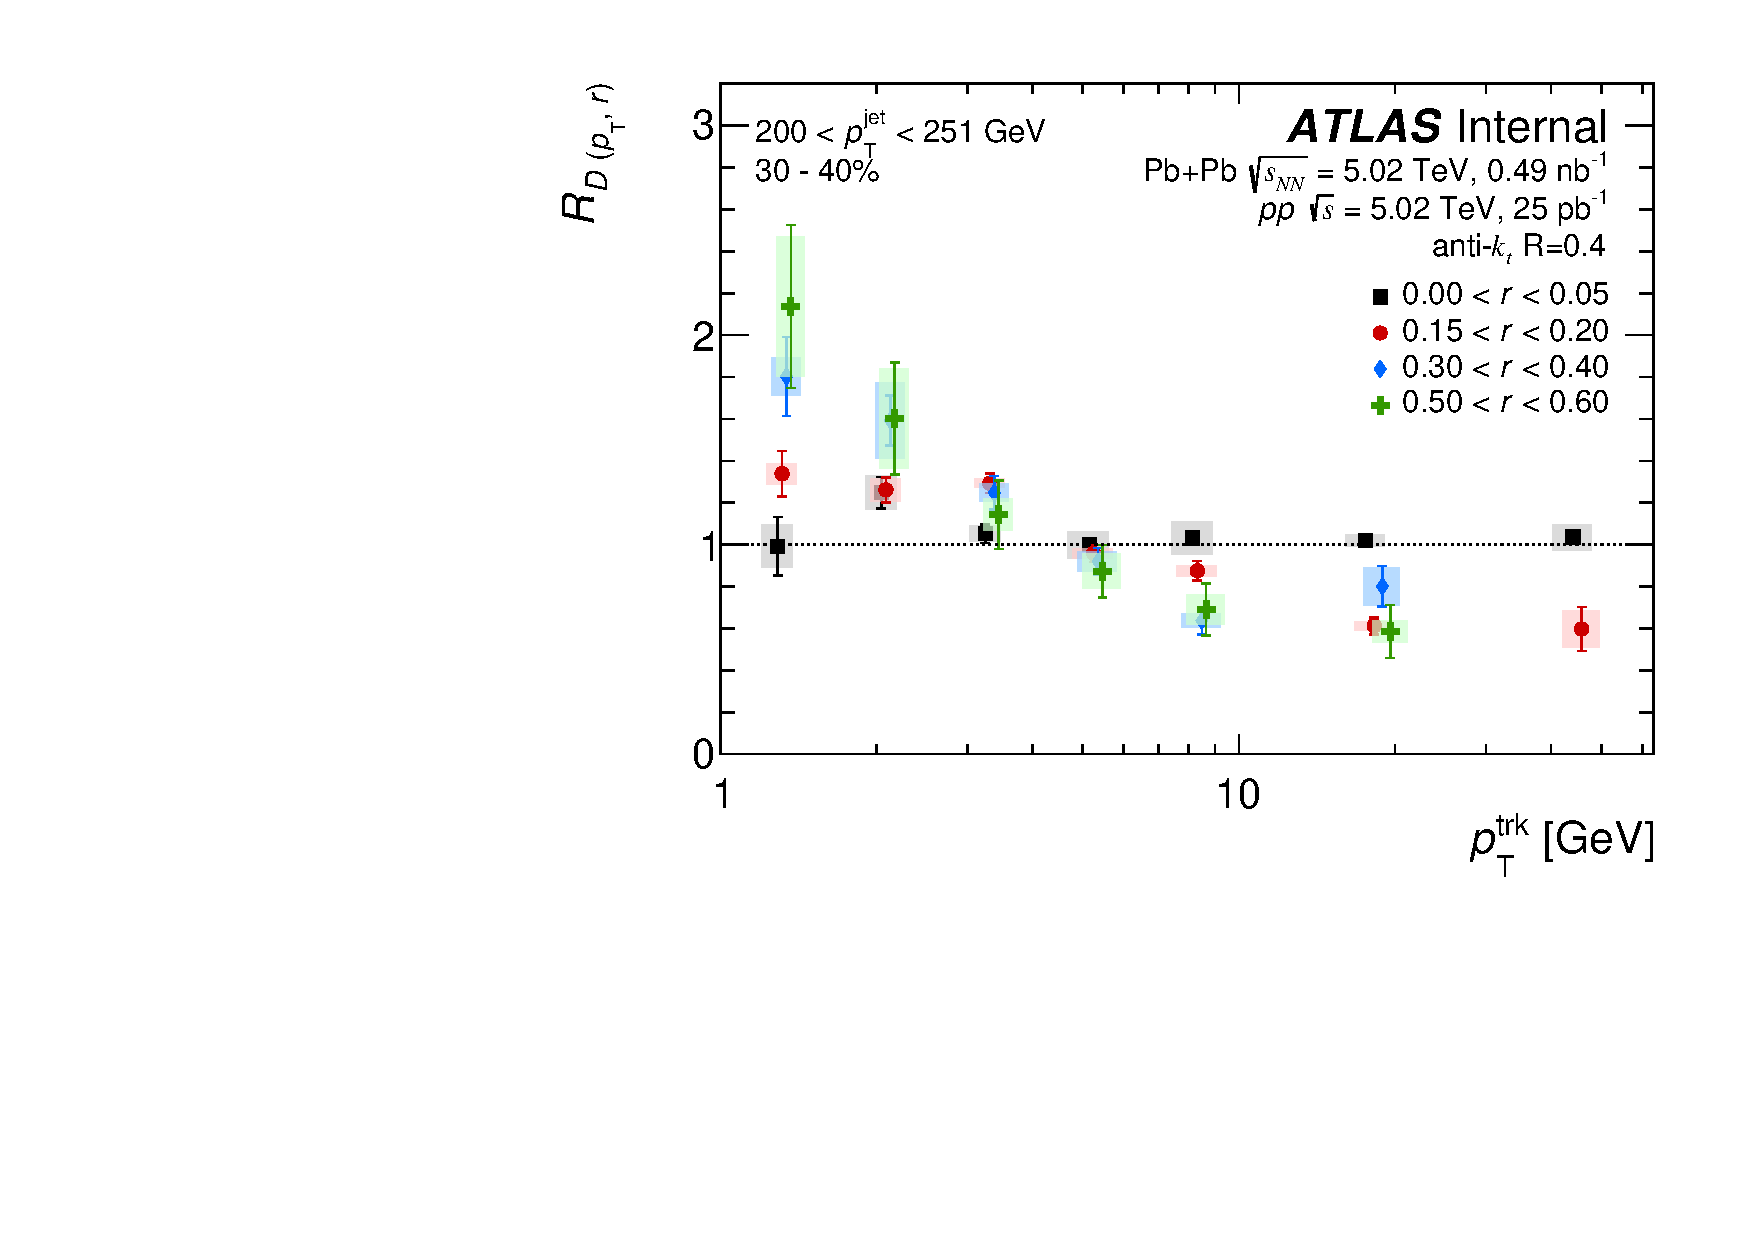
\includegraphics[width=0.5\textwidth]{results/RDpT_trkpt_jet9_cent3} \\
	 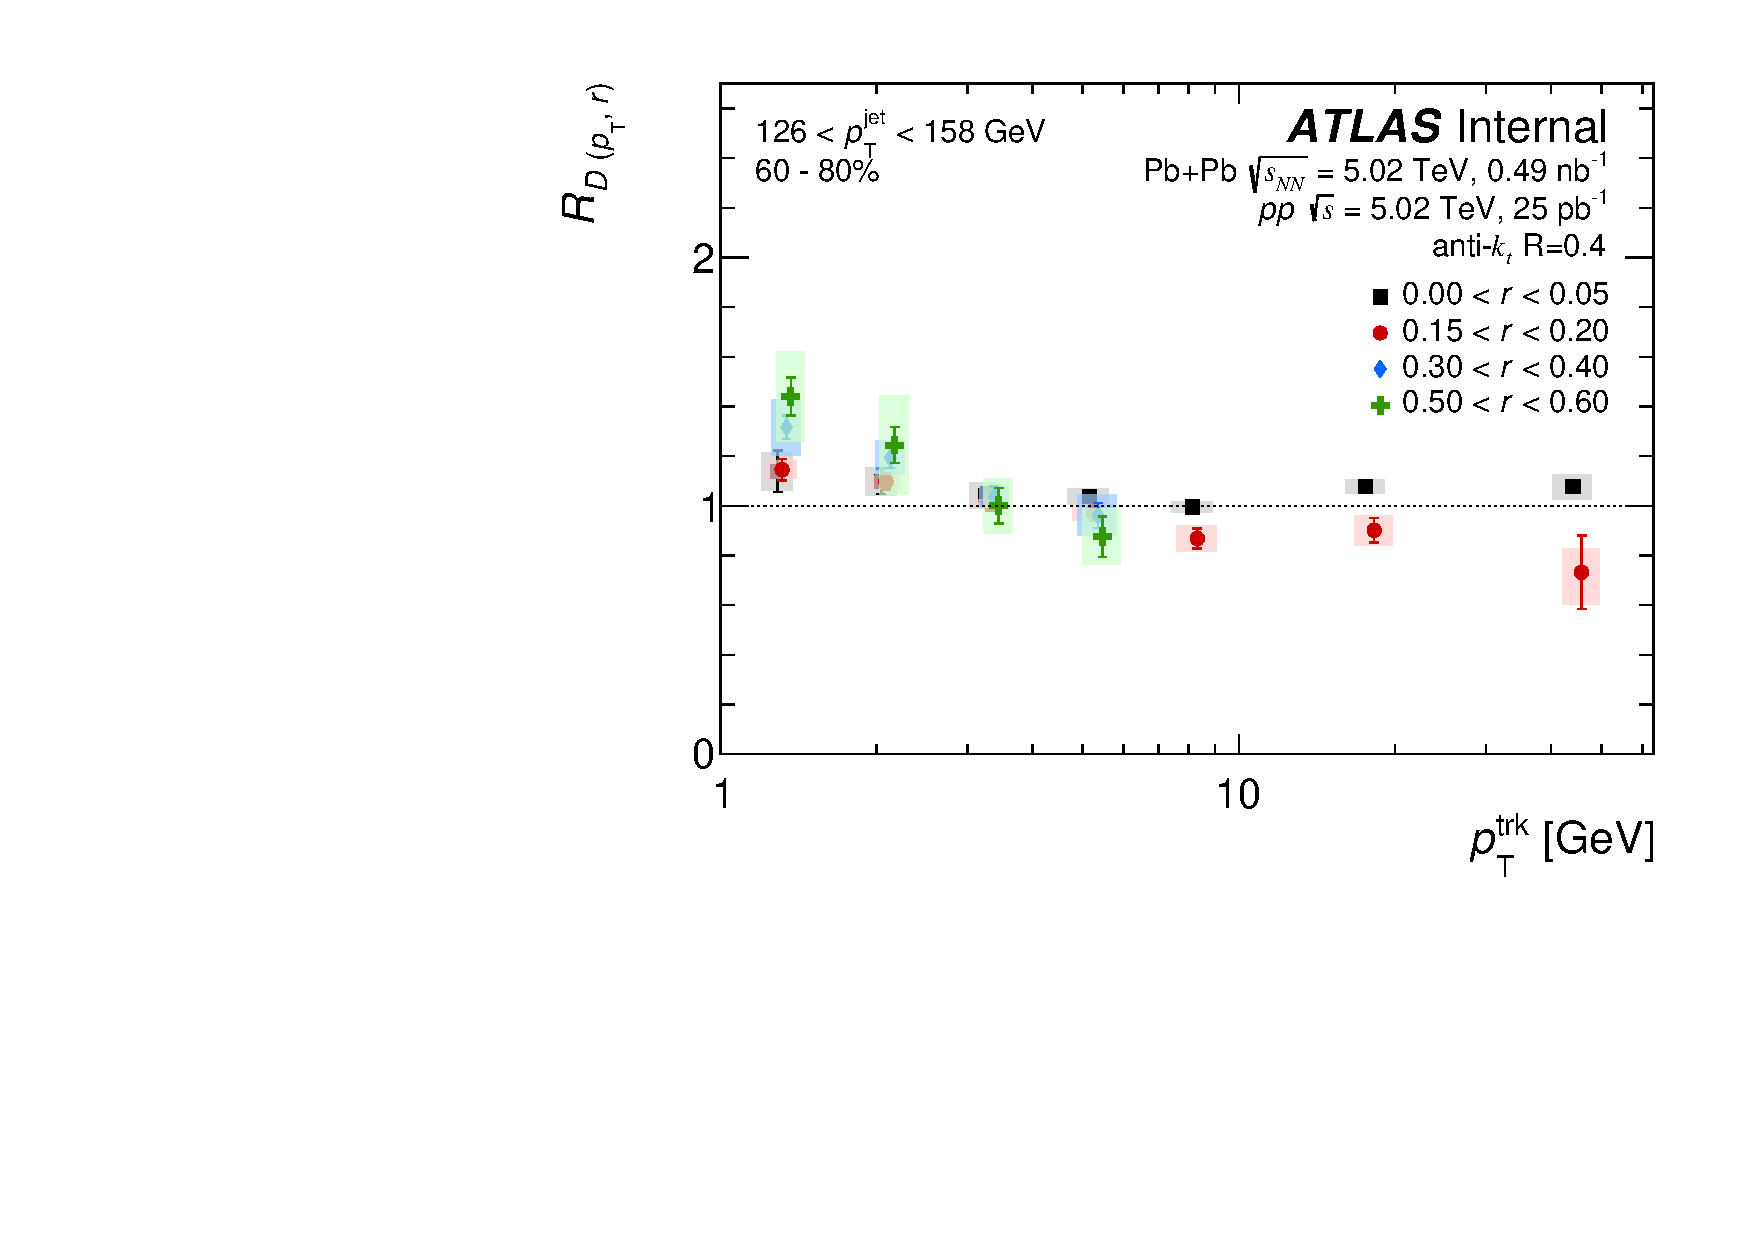
\includegraphics[width=0.5\textwidth]{results/RDpT_trkpt_jet7_cent5} &
	 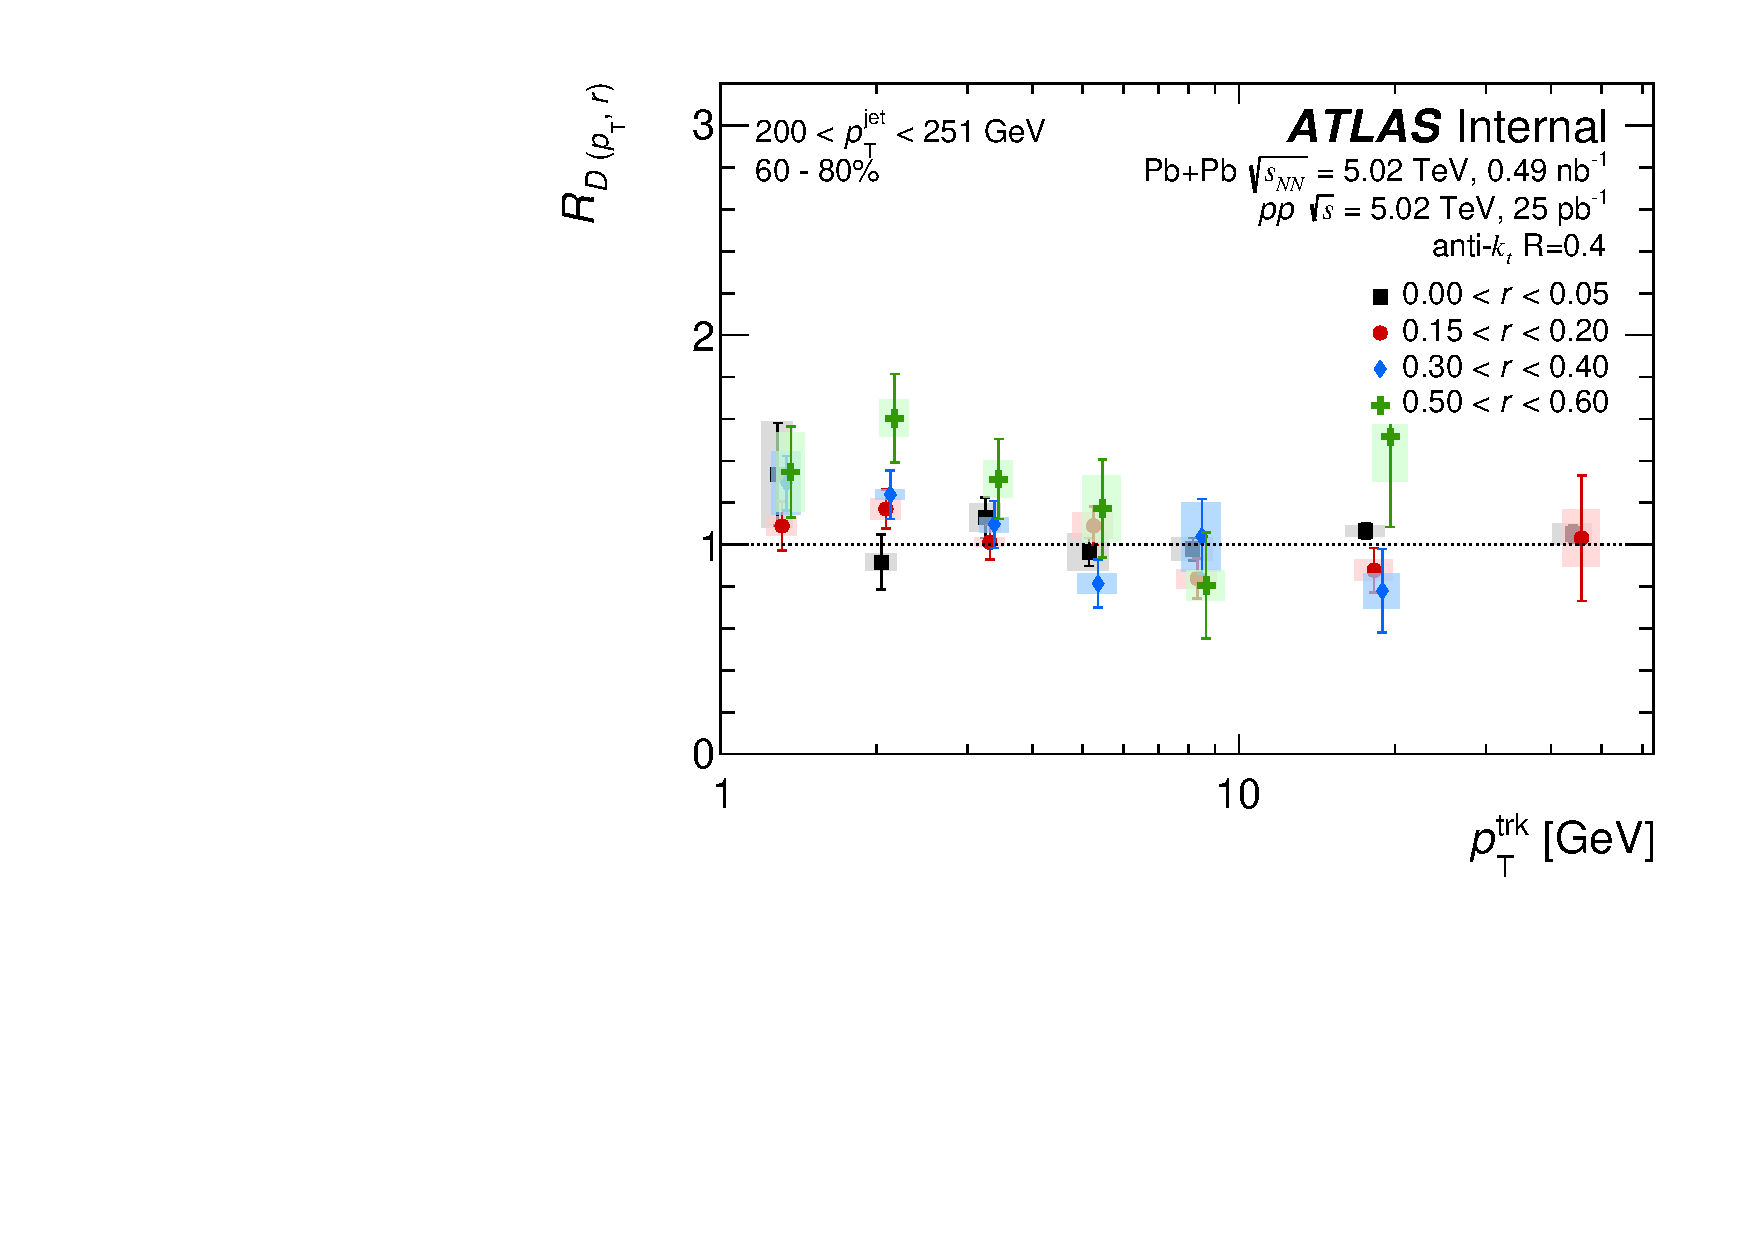
\includegraphics[width=0.5\textwidth]{results/RDpT_trkpt_jet9_cent5} \\
\end{tabular} }
   \caption{\RDptr\ as a function of \pt\ in  0--10\% (top), 30--40\% (middle), and 60--80\% (bottom) \PbPb\ collisions to \pp\ collisions for two different \ptjet\ selections: 126--158~\GeV\ (left) and 200--251~\GeV\ (right). The different colors indicate different angular distances from the jet axis. The vertical bars on the data points indicate statistical uncertainties while the shaded boxes indicate systematic uncertainties. The widths of the boxes are not indicative of the bin size and the points are shifted horizontally for better visibility.}
      \label{fig:pttrkdep}
\end{figure}

\begin{figure}
\centering{
\begin{tabular}{cc}
	 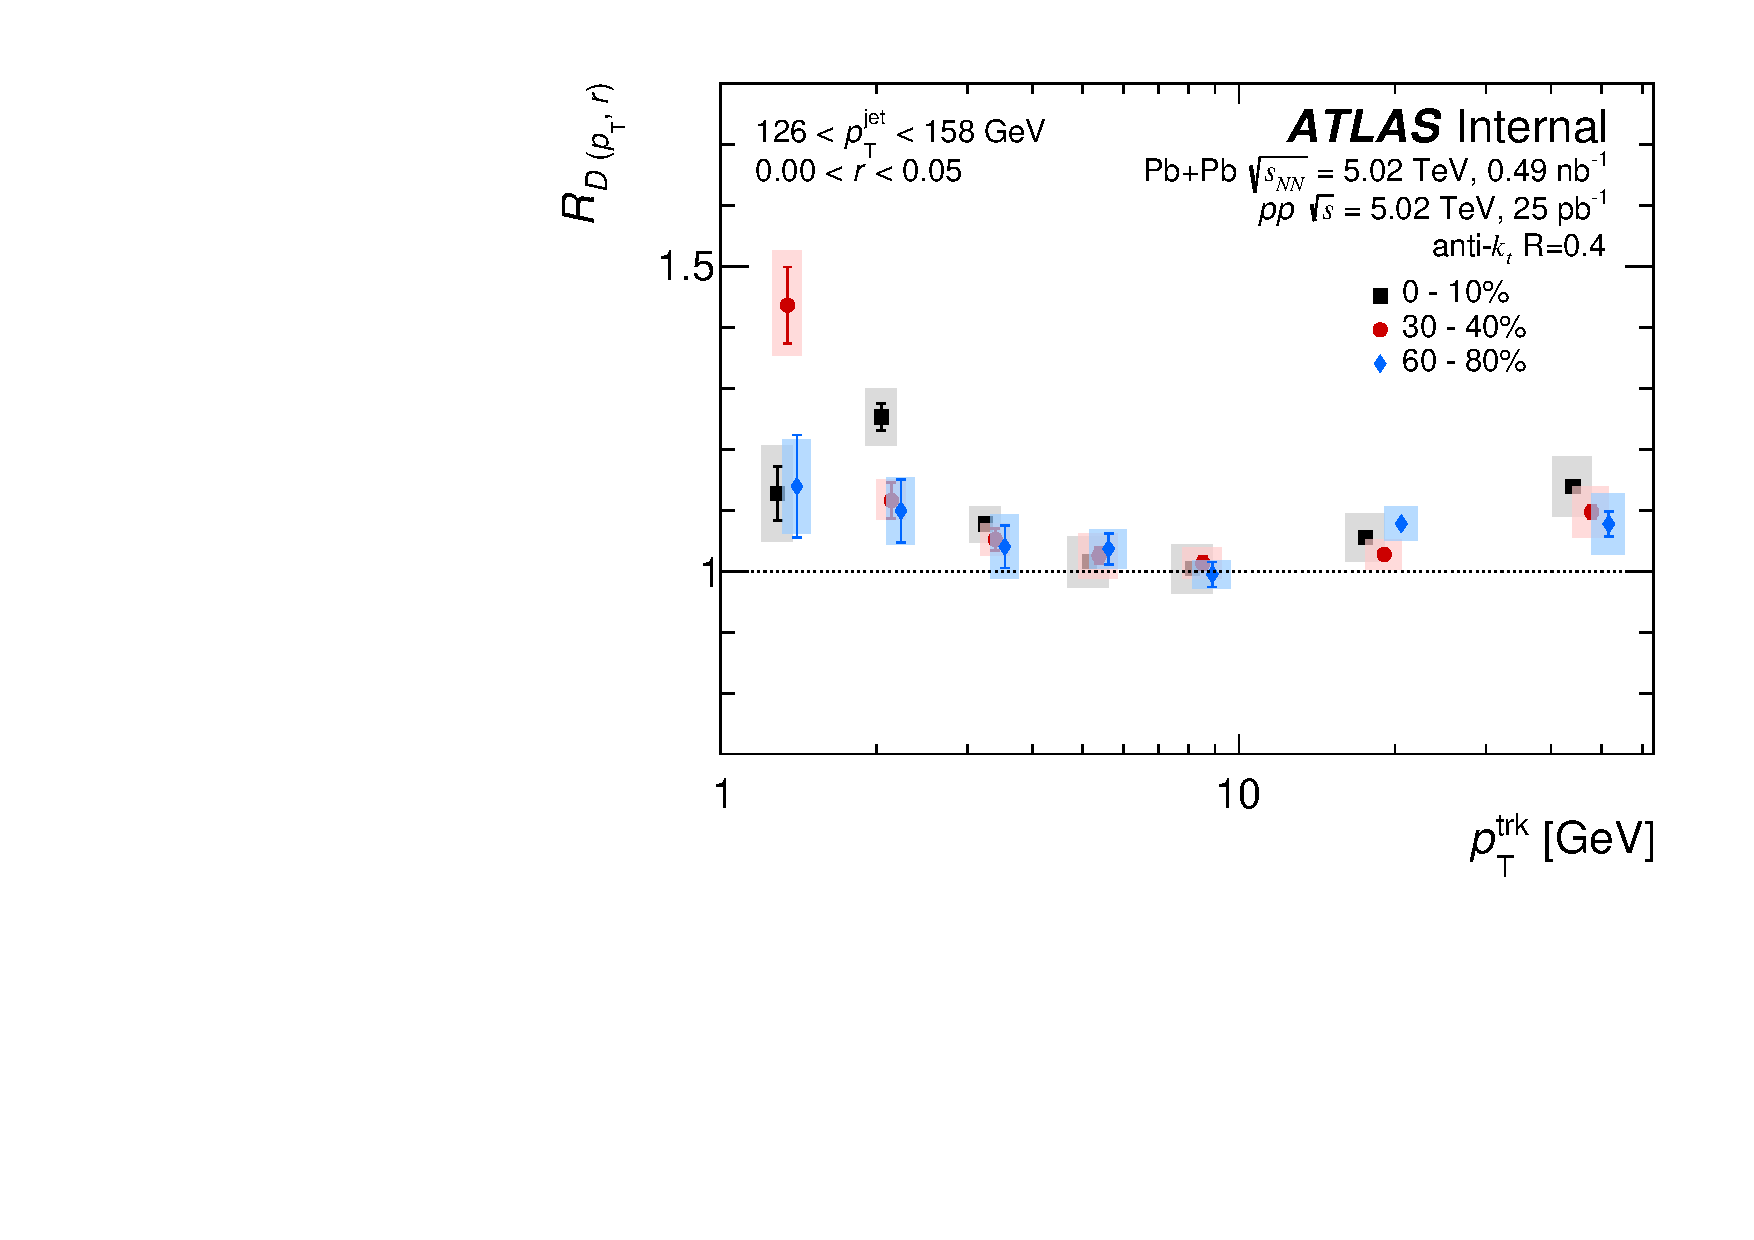
\includegraphics[width=0.5\textwidth]{results/RDpT_trkpt_jet7_dR0} &
	 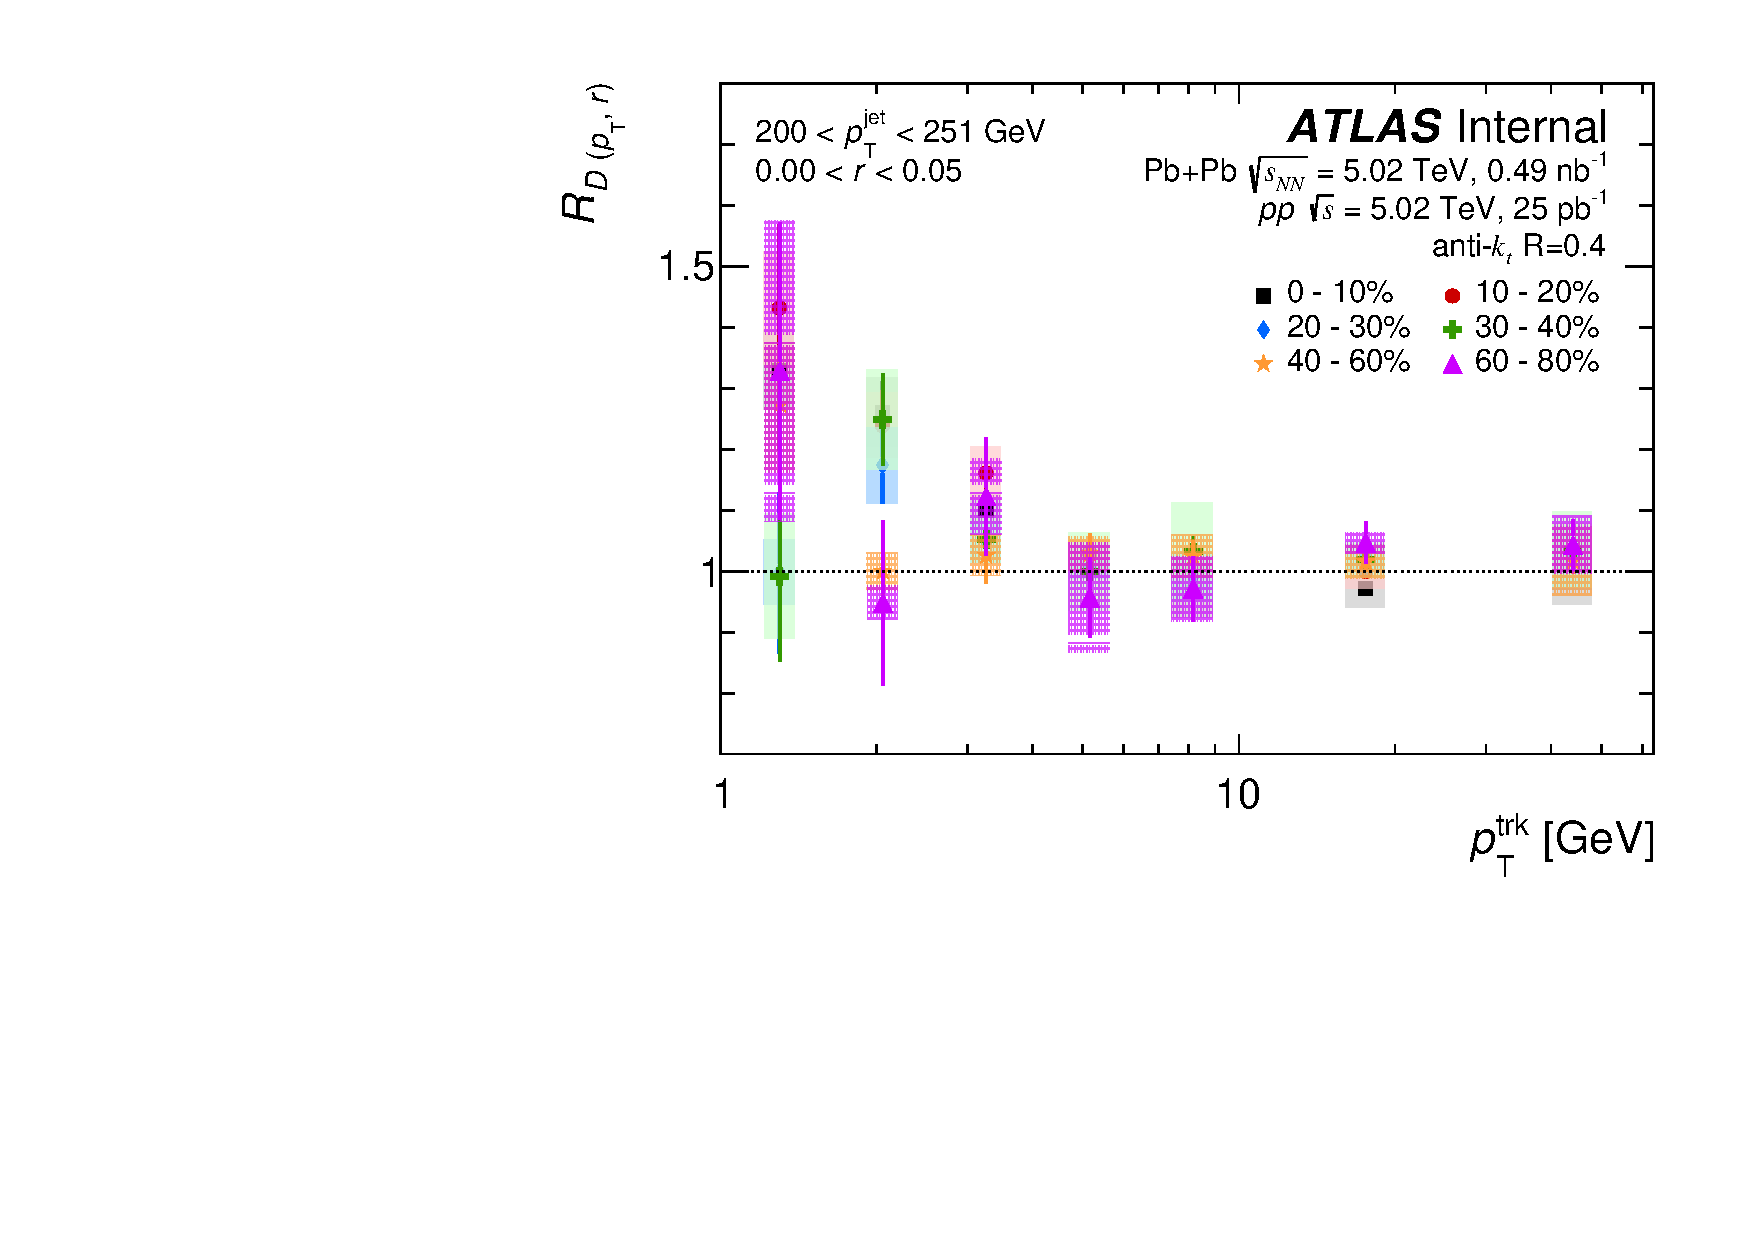
\includegraphics[width=0.5\textwidth]{results/RDpT_trkpt_jet9_dR0} \\
	 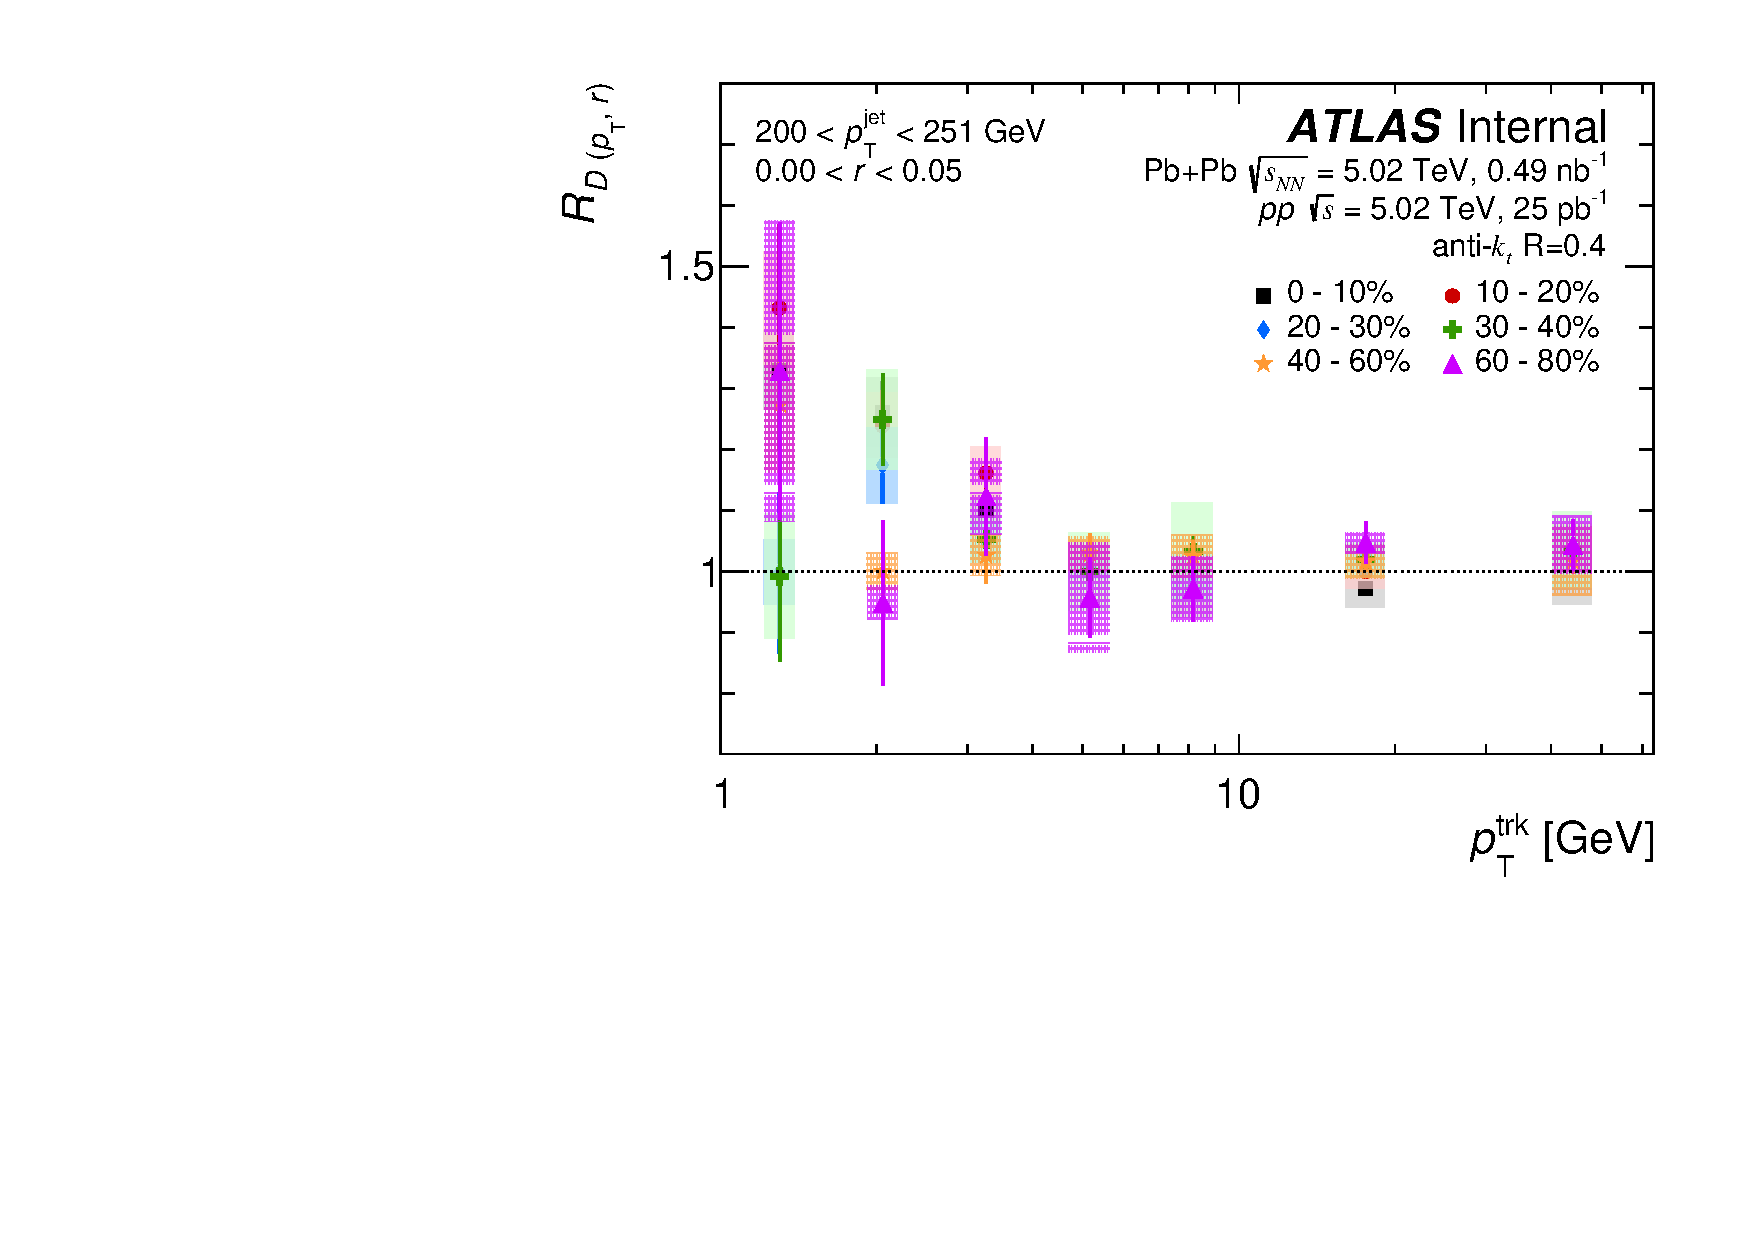
\includegraphics[width=0.5\textwidth]{results/RDpT_trkpt_jet9_dR0} &
	 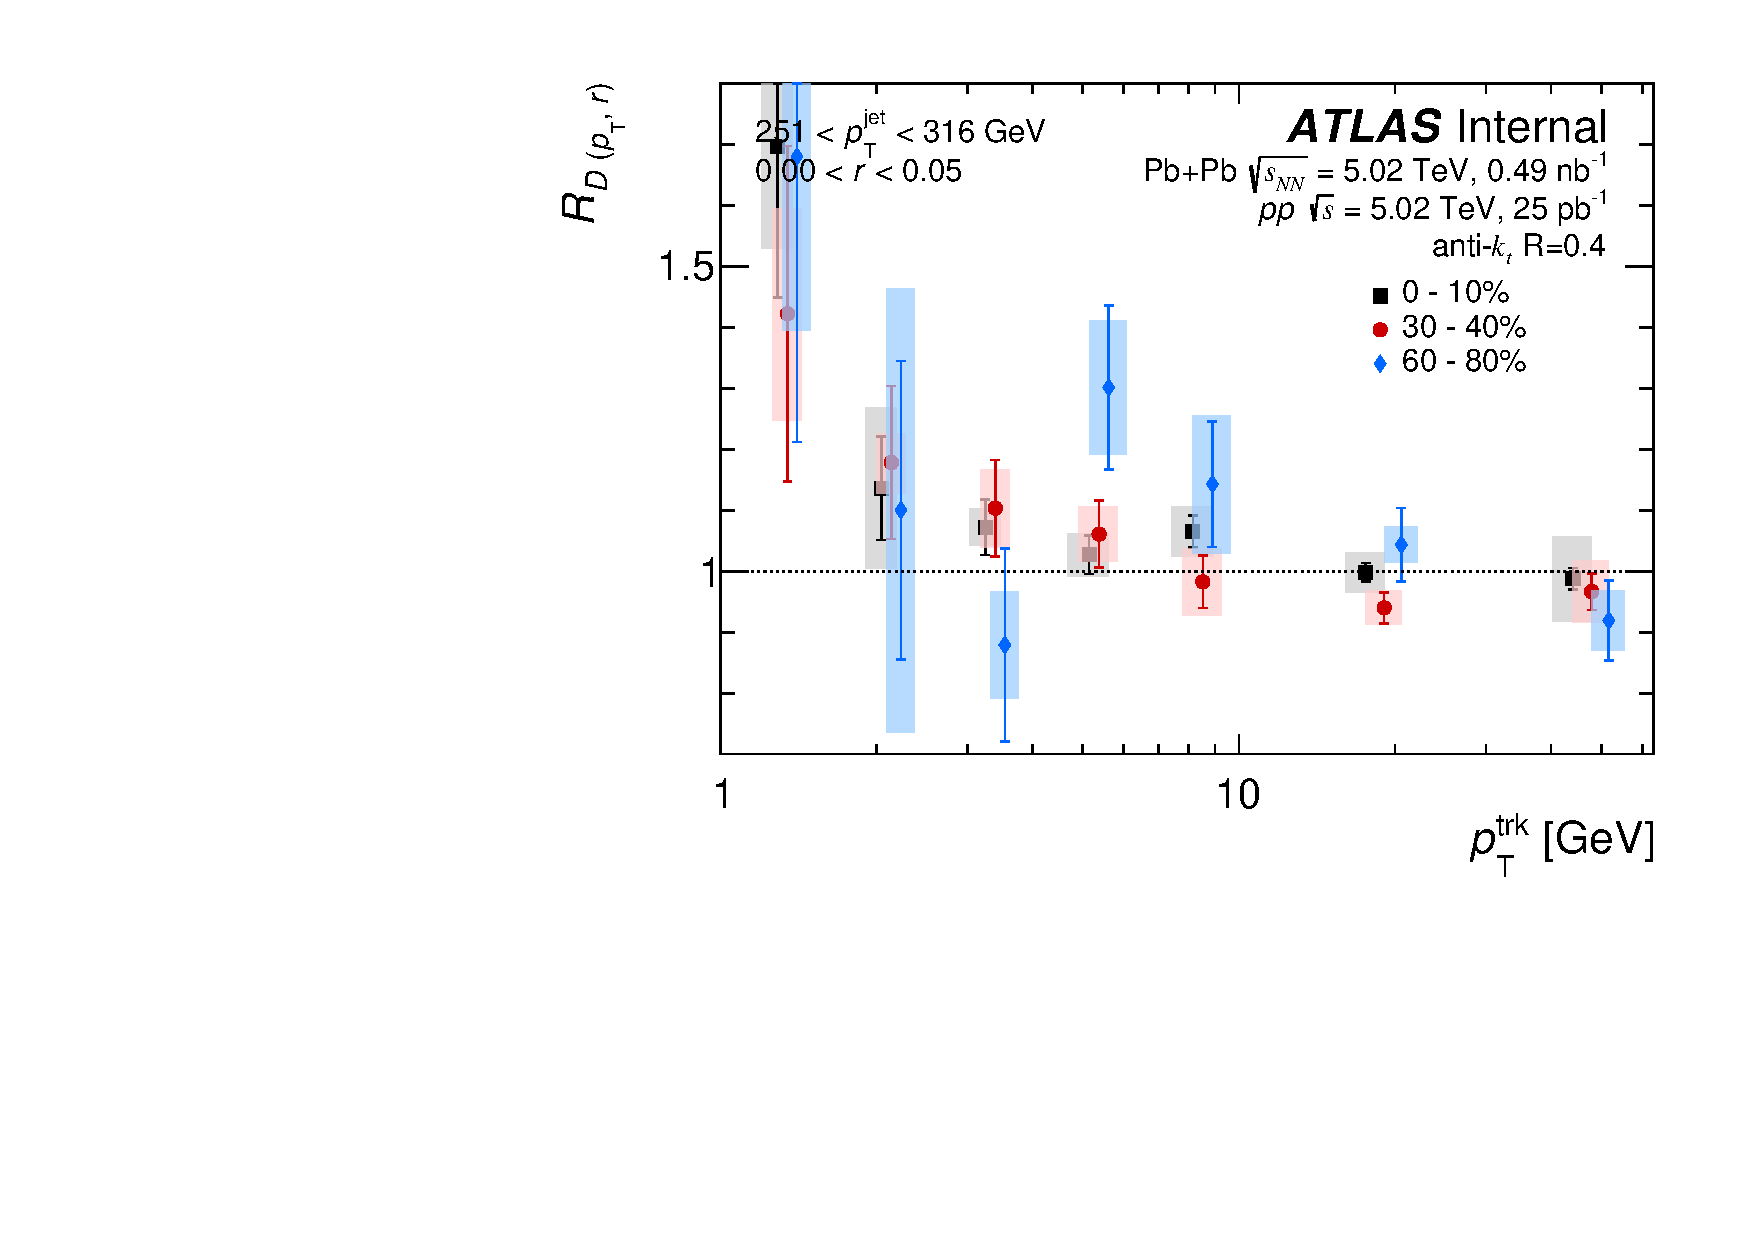
\includegraphics[width=0.5\textwidth]{results/RDpT_trkpt_jet10_dR0} \\
%	 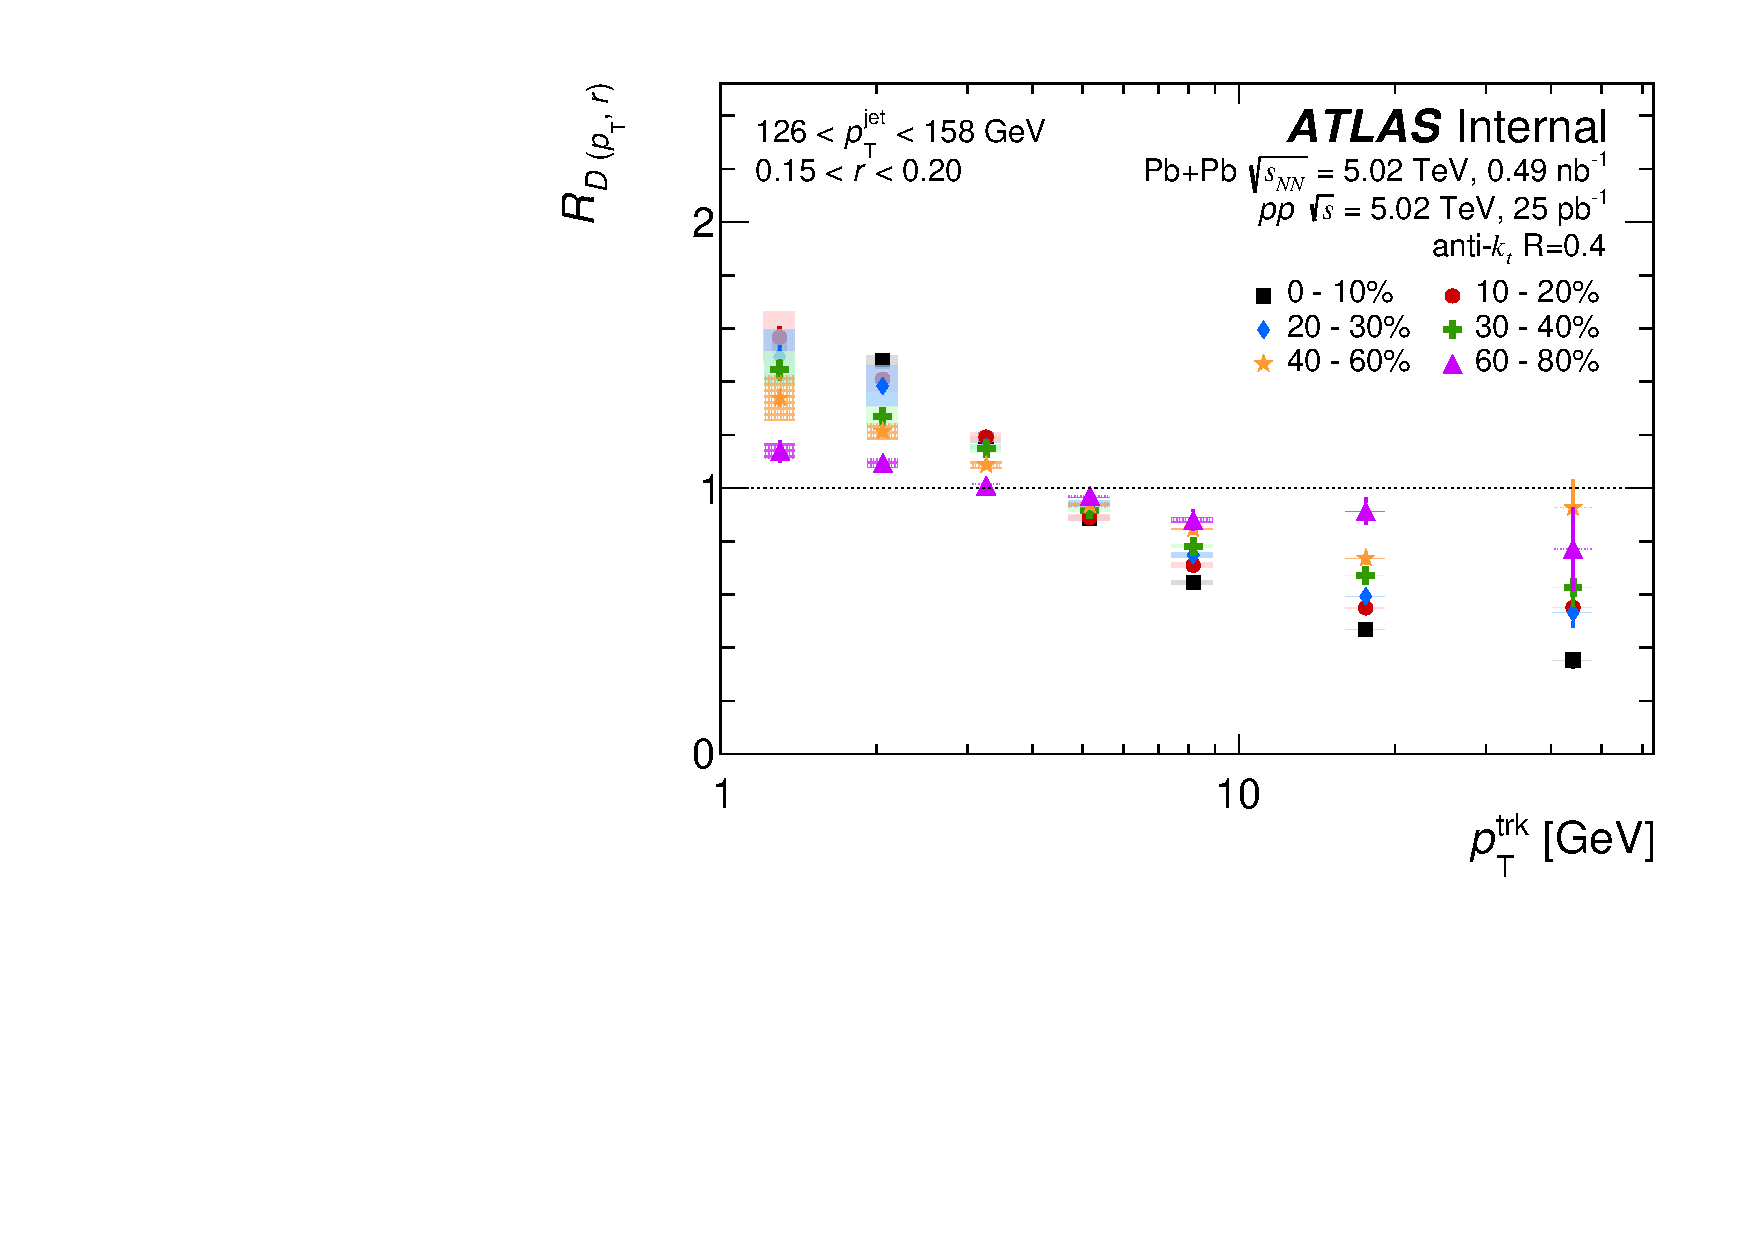
\includegraphics[width=0.5\textwidth]{results/RDpT_trkpt_jet7_dR3} &
%	 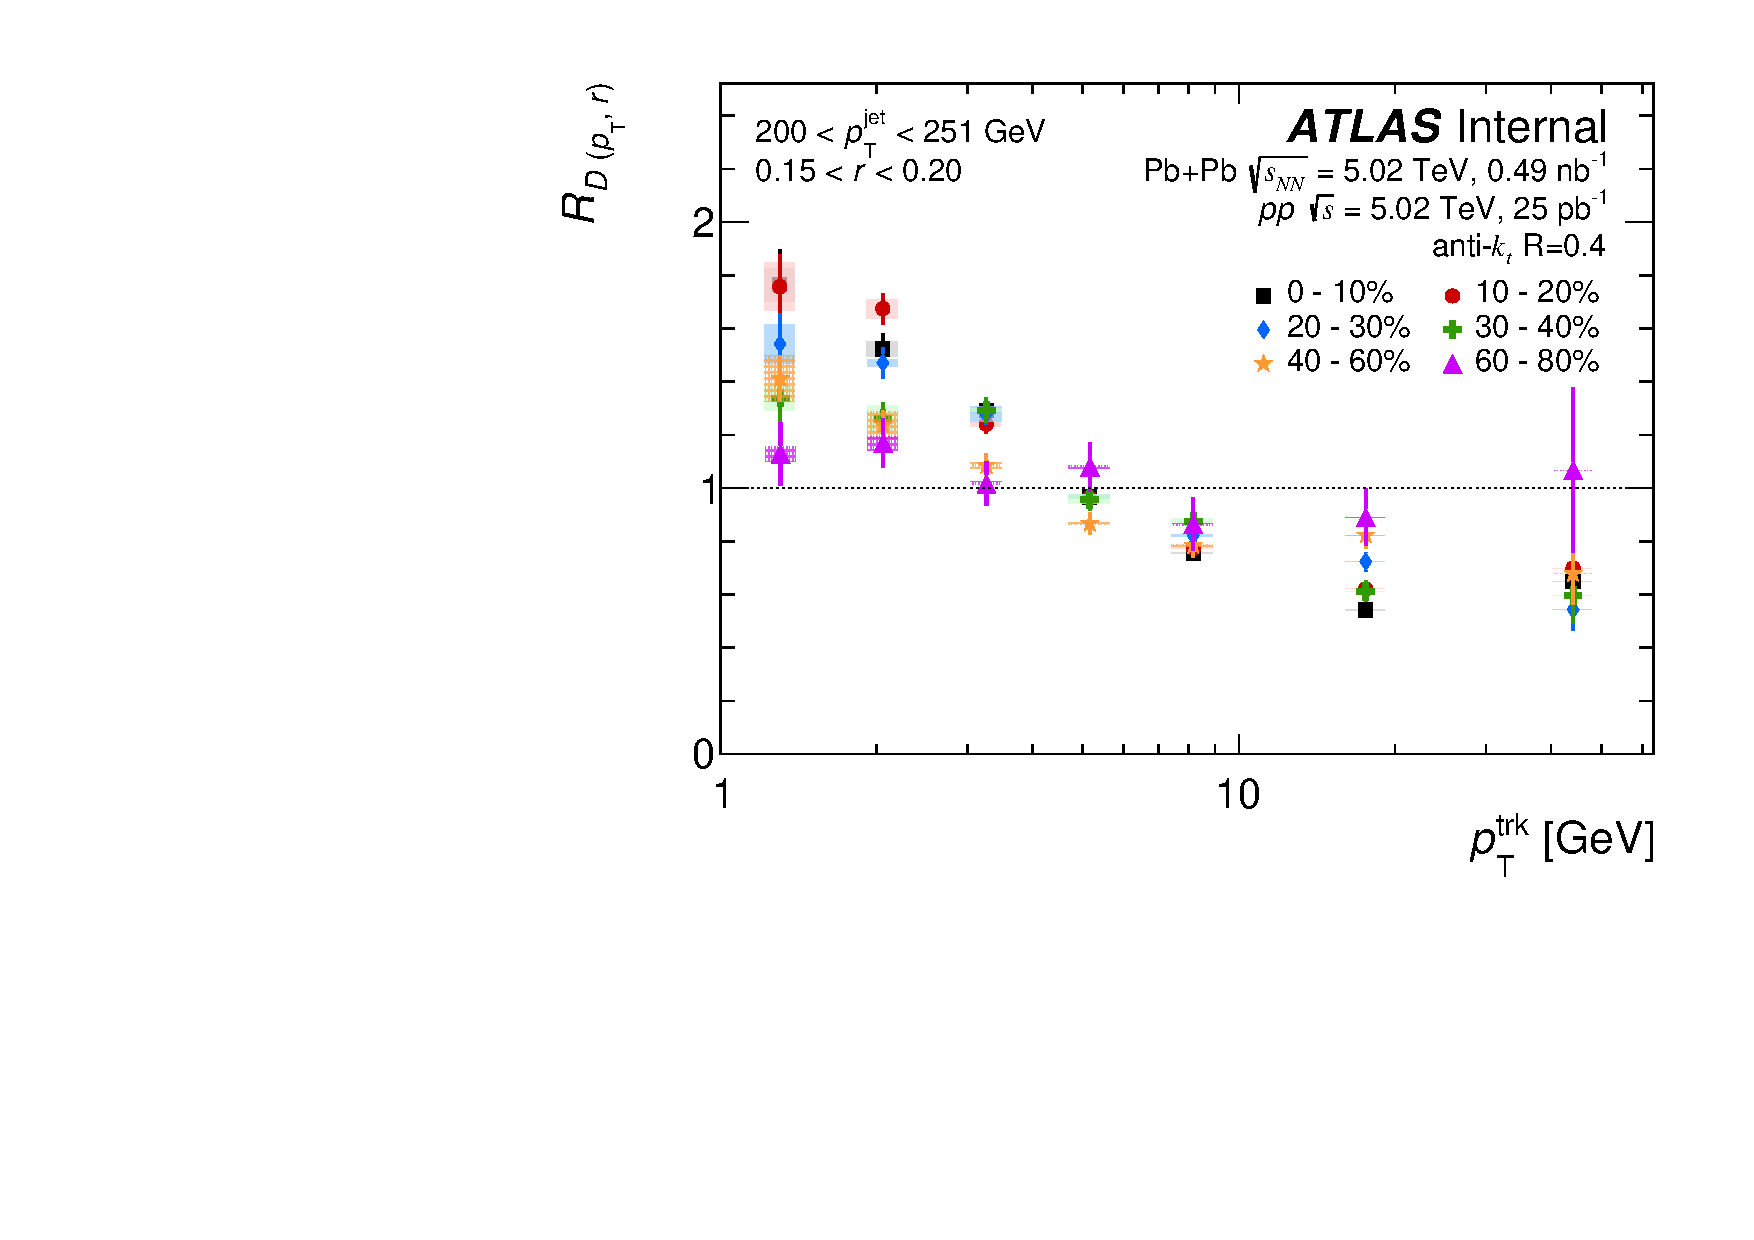
\includegraphics[width=0.5\textwidth]{results/RDpT_trkpt_jet9_dR3} \\
%	 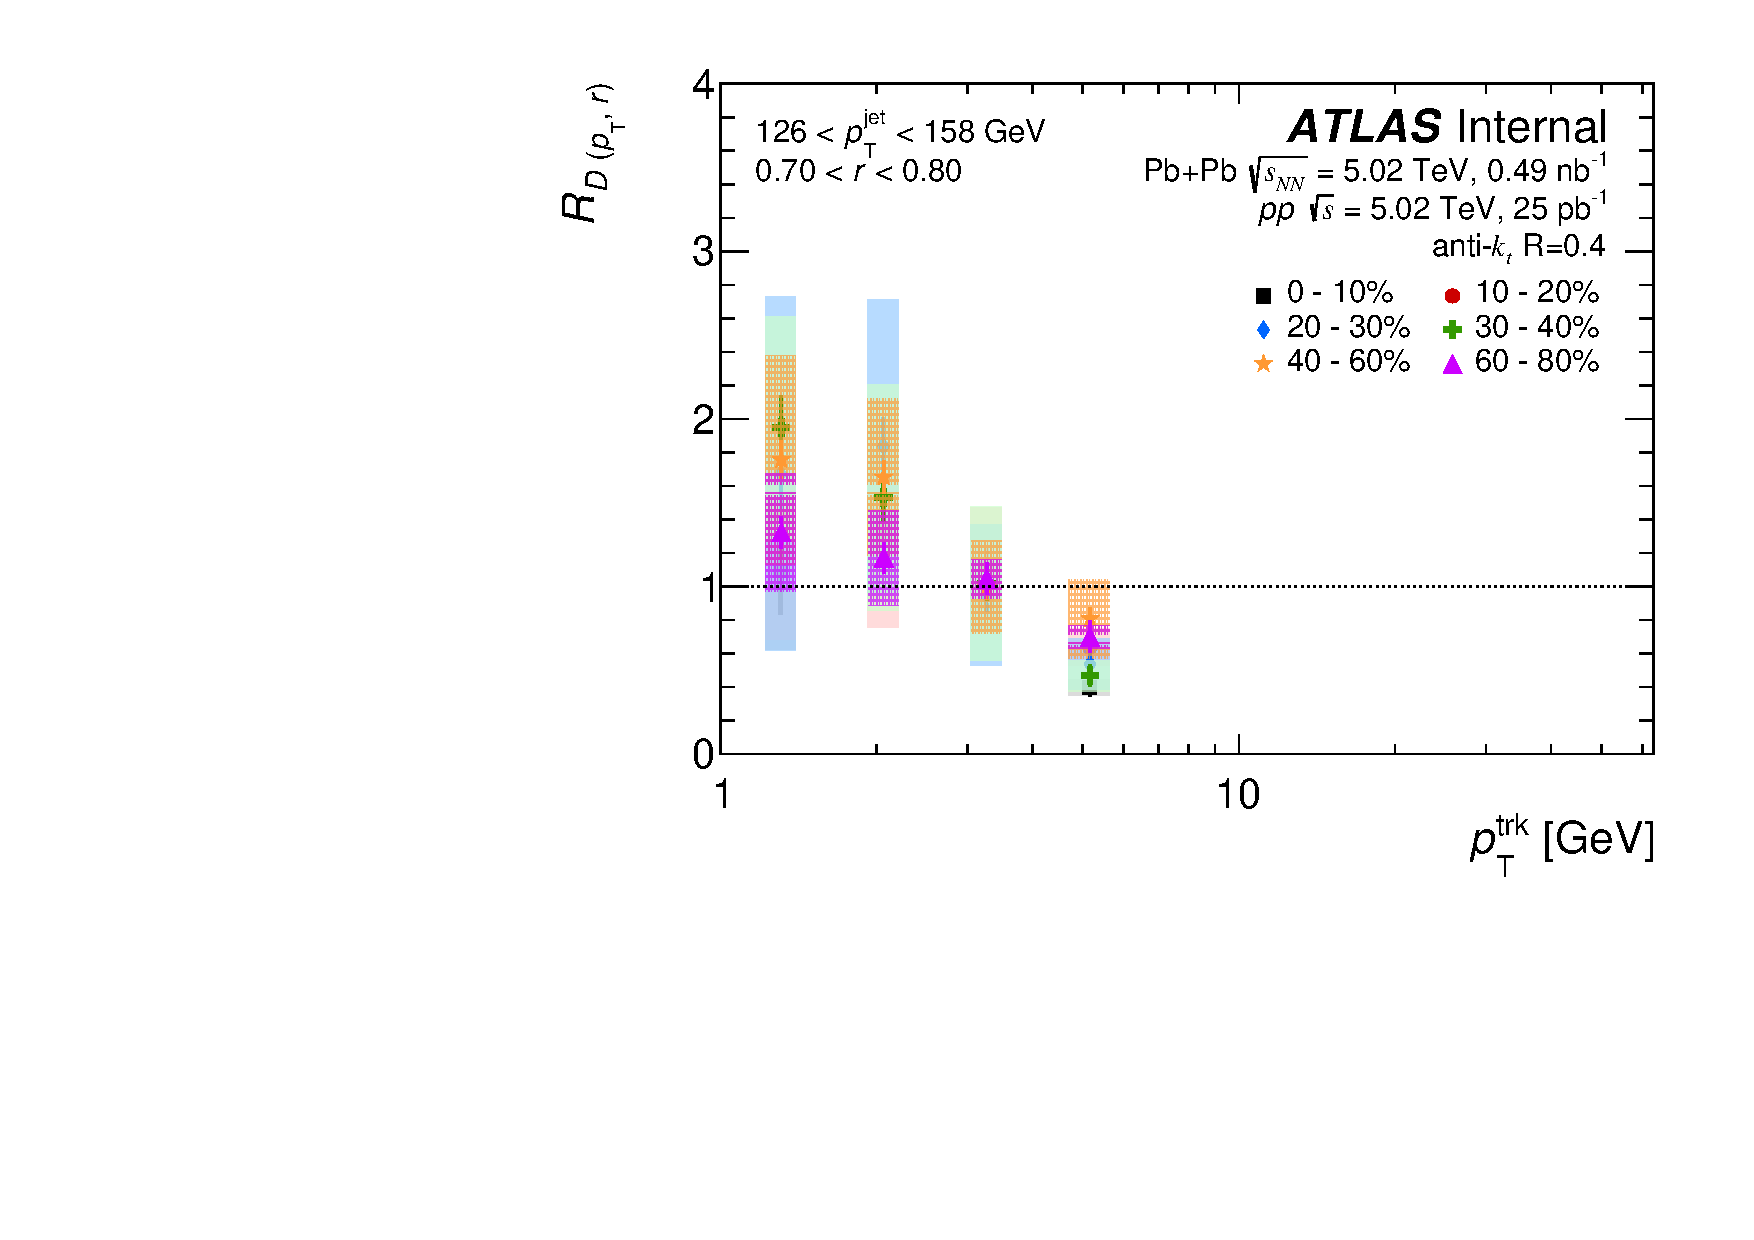
\includegraphics[width=0.5\textwidth]{results/RDpT_trkpt_jet7_dR10} &
%	 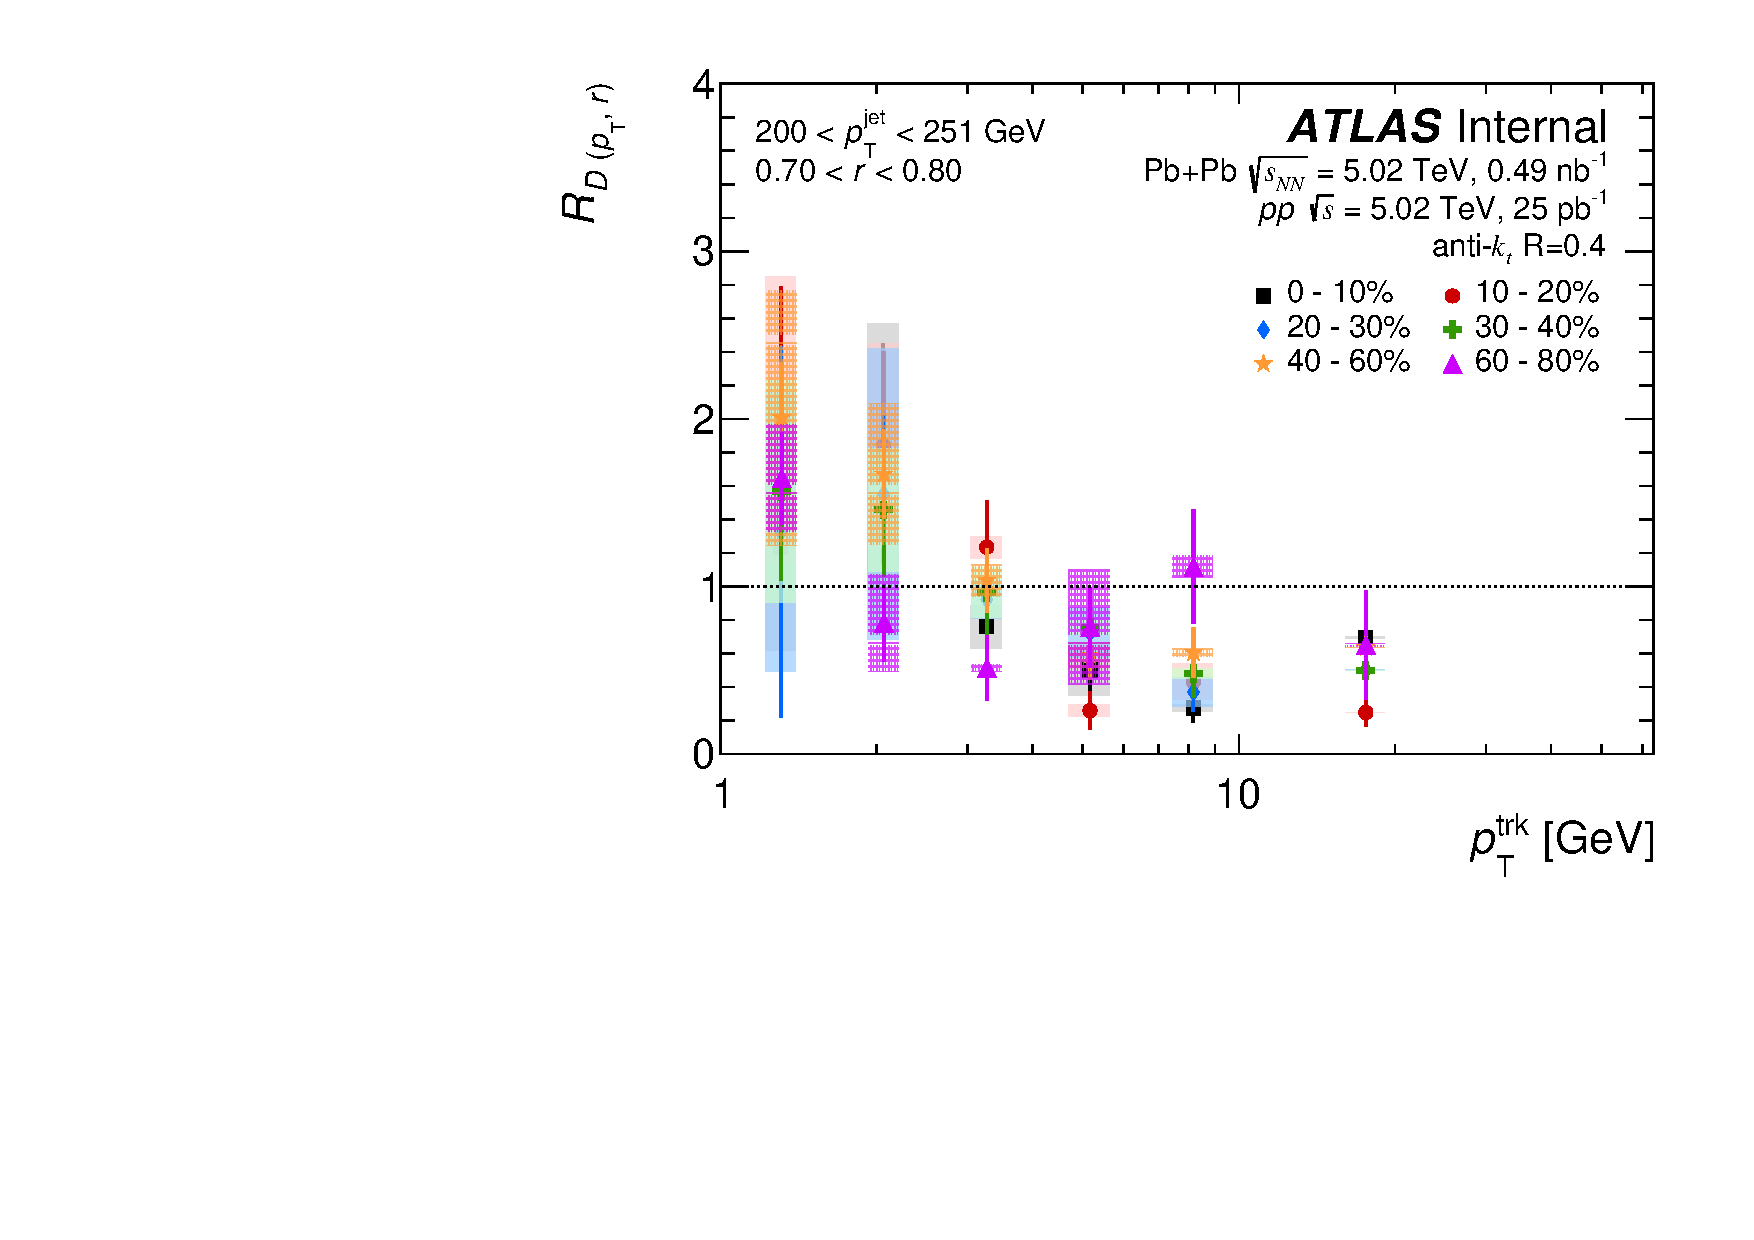
\includegraphics[width=0.5\textwidth]{results/RDpT_trkpt_jet9_dR10} \\
\end{tabular} }
   \caption{\RDptr\ for central \pbpb\ collisions as a function of \pt\ for different jet selections. The different colors represent different centrality bins. The vertical bars on the data points indicate statistical uncertainties while the shaded boxes indicate systematic uncertainties. The widths of the boxes are not indicative of the bin size and the points are shifted horizontally for better visibility.}
      \label{fig:rdptr_trk_cent}
\end{figure}
%%%%%%%%%%%%%




%% DeltaDpT
Differences between the \Dptr\ distributions in \pbpb\ and \pp, given as:

\begin{align}
\DeltaDptr = \Dptr_{\pbpb} - \Dptr_{pp}
\end{align}

are presented as a function of $r$ for different \pt\ selections in 0--10\% central collisions in Figure~\ref{fig:deltadptr}. 
These distributions indicate an excess (depletion) in the charged-particle yield density for \pbpb\ collisions compared to \pp\ collisions for charged particles with low (high) \pt. This excess ranges from 0.5 to 4 particles per unit area at 1 \GeV\ in 126--158 GeV jets for 0--10\% central \pbpb\ collisions and increases with increasing \ptjet. The depletion for high \pt\ particles is at most 0.5 particles per unit area for 126--158 GeV jets in  0--10\% central \pbpb\ collisions and increases for higher \ptjet. There is a minima in the \DeltaDptr distribution for charged particles with \mbox{$\pt >  4$} GeV at $0.05 < \rvar < 0.10$ that is seen at all \ptjet\ ranges under investigation.

\begin{figure}
\centering{
\begin{tabular}{cc}
	 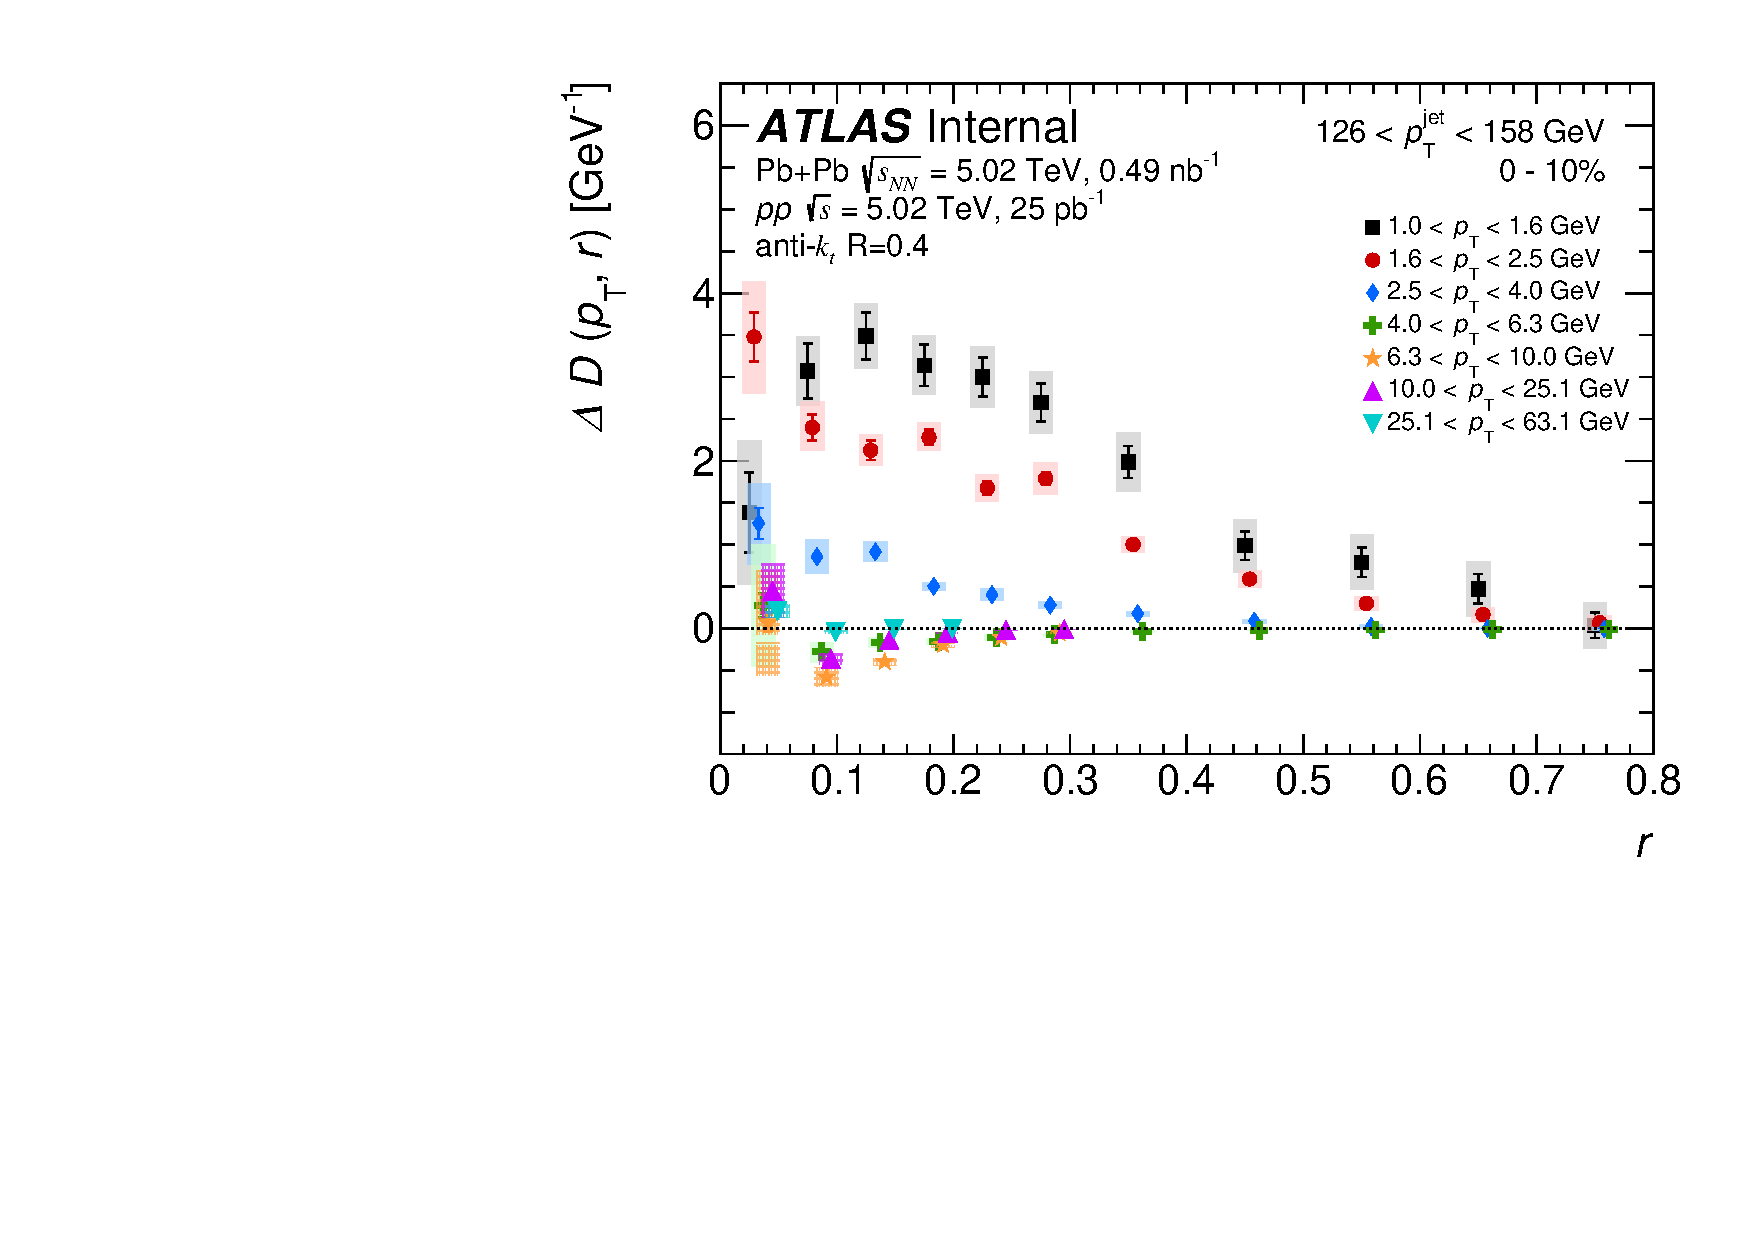
\includegraphics[width=0.5\textwidth]{results/DeltaDpT_dR_jet7_cent0} &
	 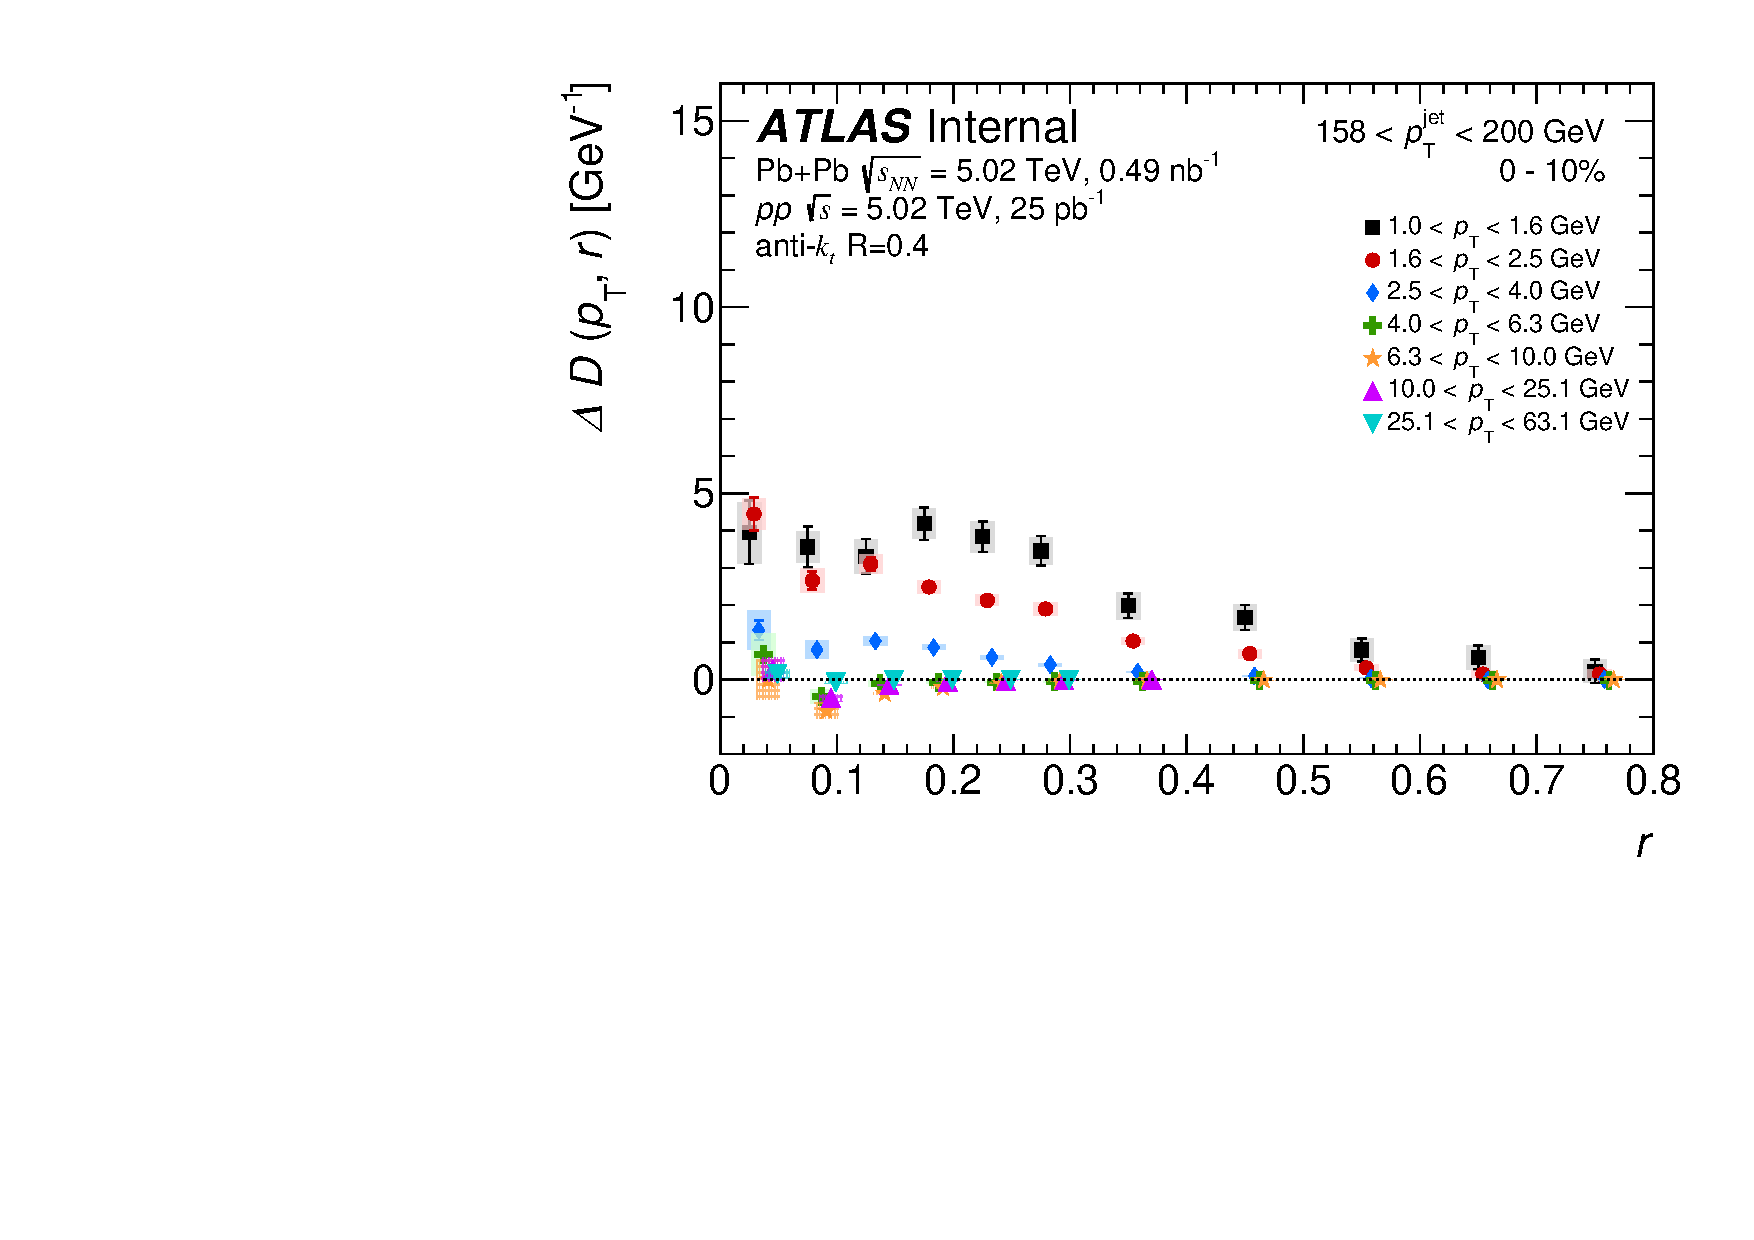
\includegraphics[width=0.5\textwidth]{results/DeltaDpT_dR_jet8_cent0} \\
	 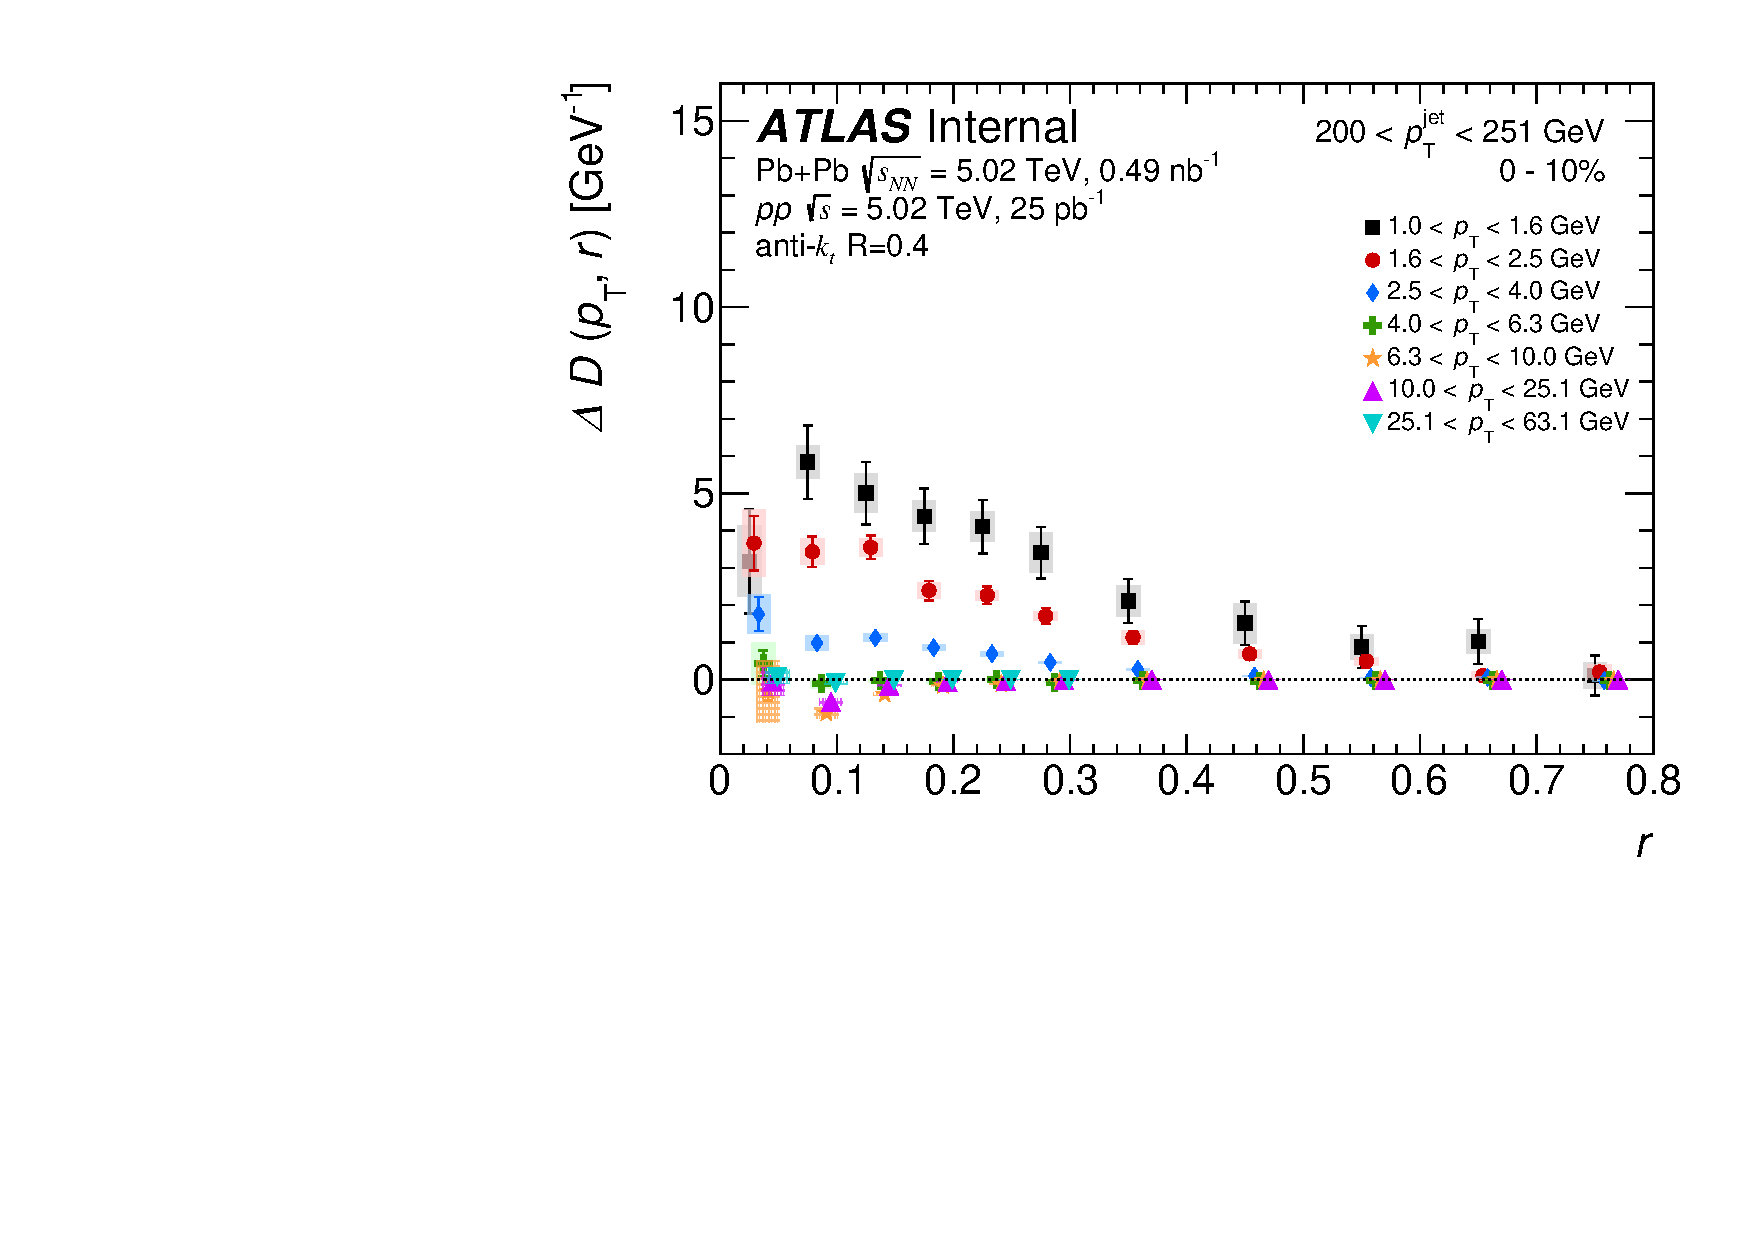
\includegraphics[width=0.5\textwidth]{results/DeltaDpT_dR_jet9_cent0} &
	 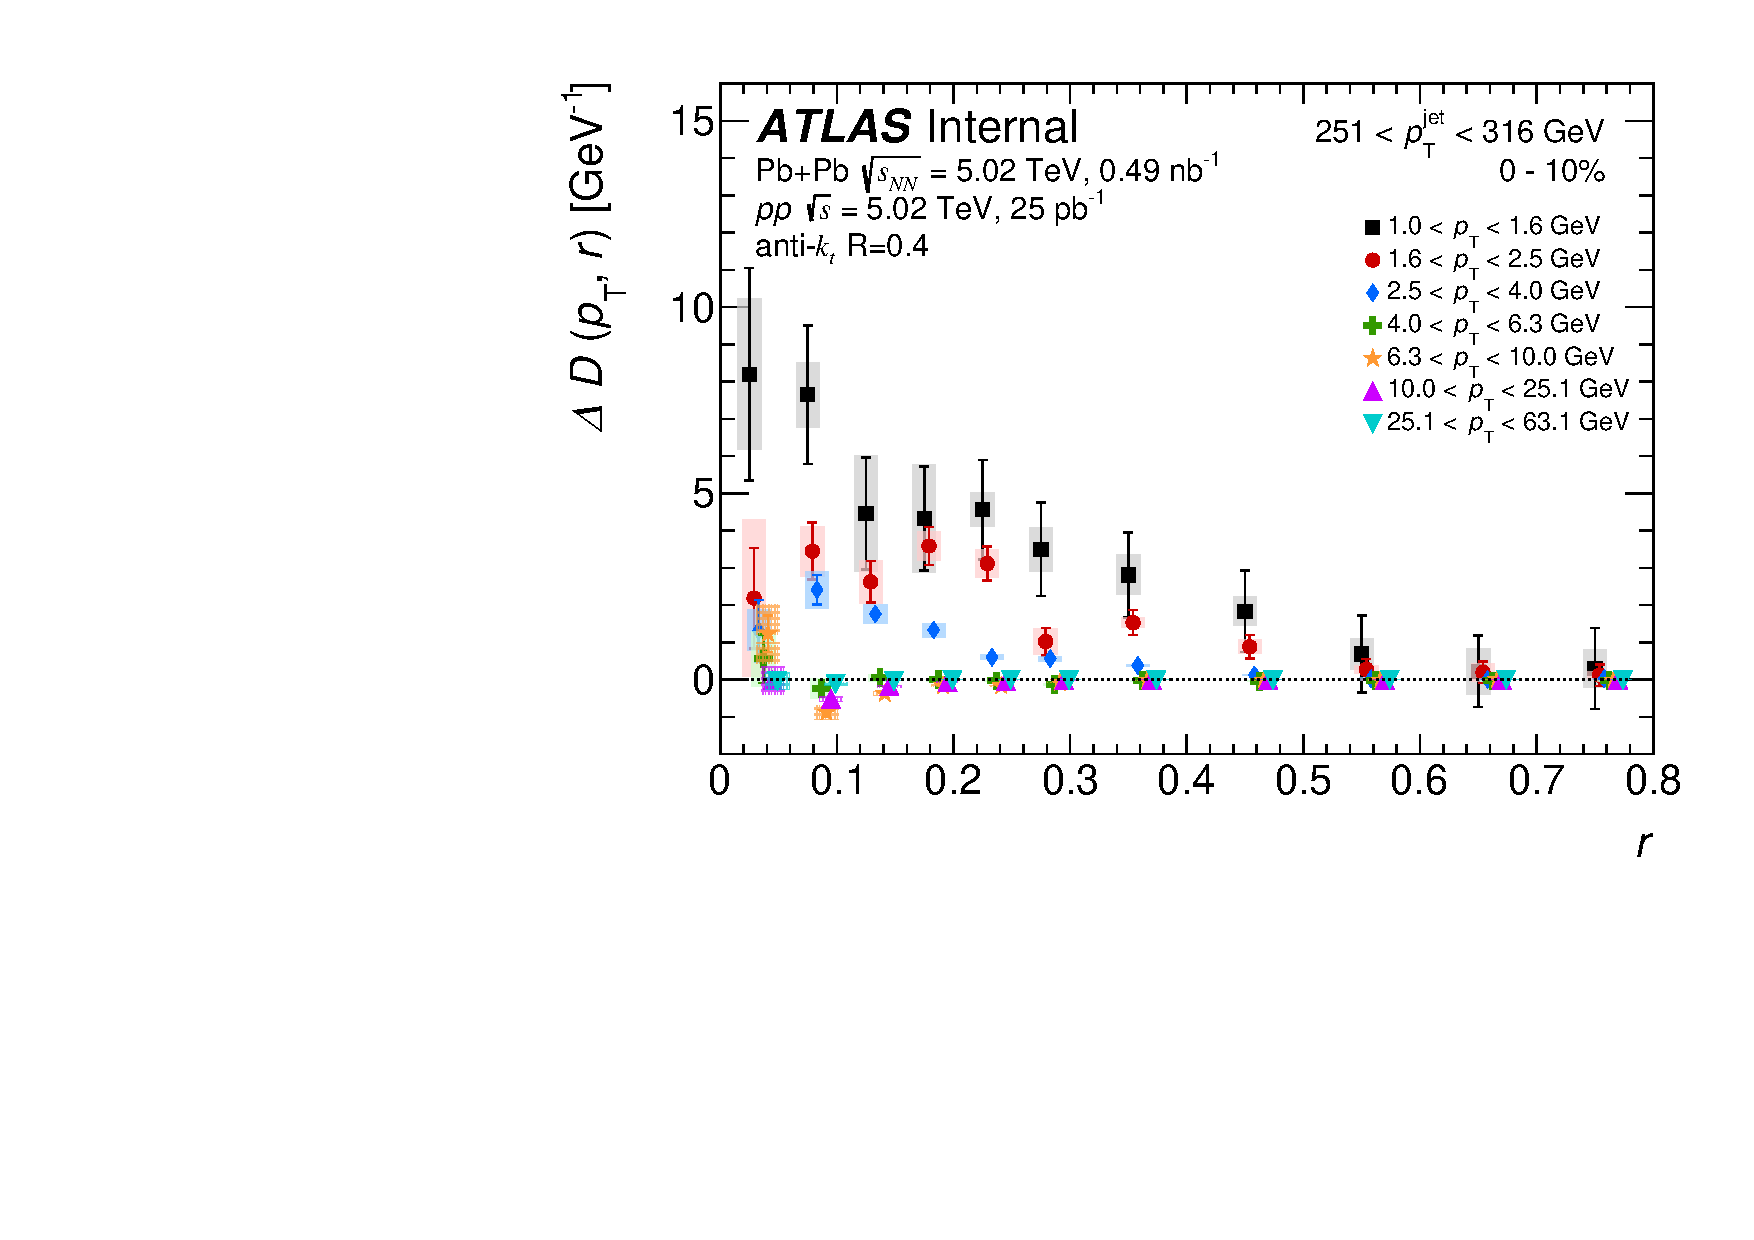
\includegraphics[width=0.5\textwidth]{results/DeltaDpT_dR_jet10_cent0} \\
\end{tabular} }
   \caption{\DeltaDptr\ as a function of \rvar\ in central collisions for all \pt\ ranges in four \ptjet\ selections: 126--158~\GeV, 158--200~\GeV, 200--251~\GeV, and 251--316~\GeV. The vertical bars on the data points indicate statistical uncertainties while the shaded boxes indicate systematic uncertainties. The widths of the boxes are not indicative of the bin size and the points are shifted horizontally for better visibility. }
      \label{fig:deltadptr}
\end{figure}
%%%%%%%%%%%%%

%\subparagraph{Integrated plots}
The \Dptr\ distribution can be integrated for particles with \pt\ < 4 GeV to construct the quantities $\Theta$ and $P$.
\begin{align}
\Theta_{\mathrm{x}} &= \int_1^{4} \Dptr |_{\mathrm{x}} \\
P_{\mathrm{x}} &= \int_0^r \int_1^{4} \Dptr \fd \pt \fd r' |_{\mathrm{x}}
\end{align}
where x $\in [\pp, \pbpb]$. These can be compared between the \pp\ and \pbpb\ systems to give the following distributions:
\begin{align}
\Delta_\Theta = \Theta_{\mathrm{Pb+Pb}} - \Theta_{pp} & \qquad  \Delta_P = P_{\mathrm{Pb+Pb}} - P_{pp} \\
R_\Theta = \frac{\Theta_{\mathrm{Pb+Pb}}}{\Theta_{\mathrm{Pb+Pb}}} & \qquad R_P = \frac{P_{\mathrm{Pb+Pb}}}{P_{pp}}
\end{align}
These variables provide aggregate information for particles with \pt < 4 GeV, both differentially and cumulatively in \rvar.
Figure~\ref{fig:deltaPdeltaT} shows the \DeltaTheta\ and \DeltaP\ distributions as a function of \rvar. The \ptjet\ dependence to the excess in charged-particle density can be seen clearly. Moreover, the \DeltaP\ distribution shows that there is an extra particle density of 0.5 when integrated up to $\rvar = 0.8$ around the jet cone. 

Figure~\ref{fig:RPRT} shows the \RTheta\ and \RP\ distributions as a function of \rvar. 


\subparagraph{Delta D Low pT integral: } See Figure \ref{fig:fullset_deltadptr_lowpT}
\begin{align}
\Delta_\Theta = \int_1^{4} \Dpt_{\mathrm{PbPb}} - \Dpt_{\mathrm{pp}} \fd \pt
\end{align}
\begin{figure}
\centering{
\begin{tabular}{cc}
	 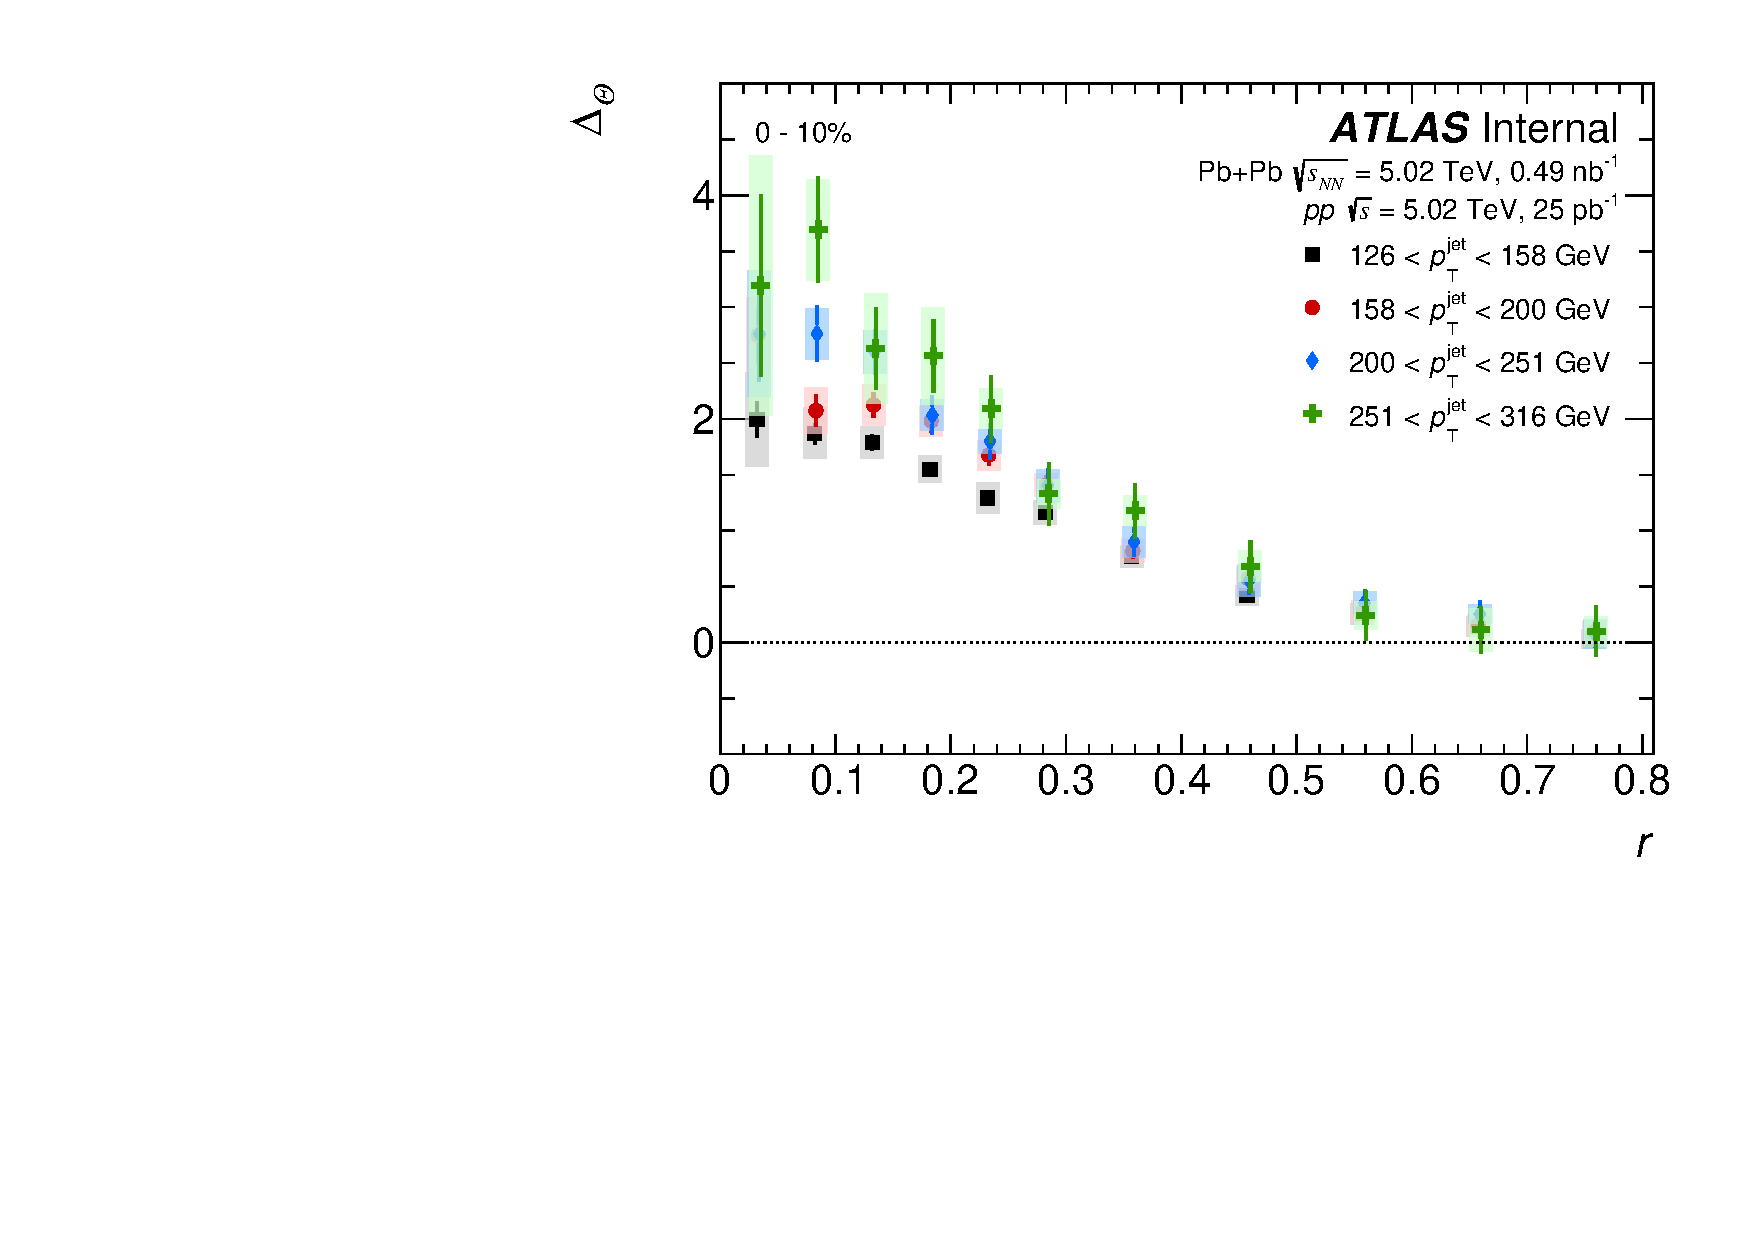
\includegraphics[width=0.5\textwidth]{results/DeltaDpT_lowpt_integ_cent0.pdf} &
	 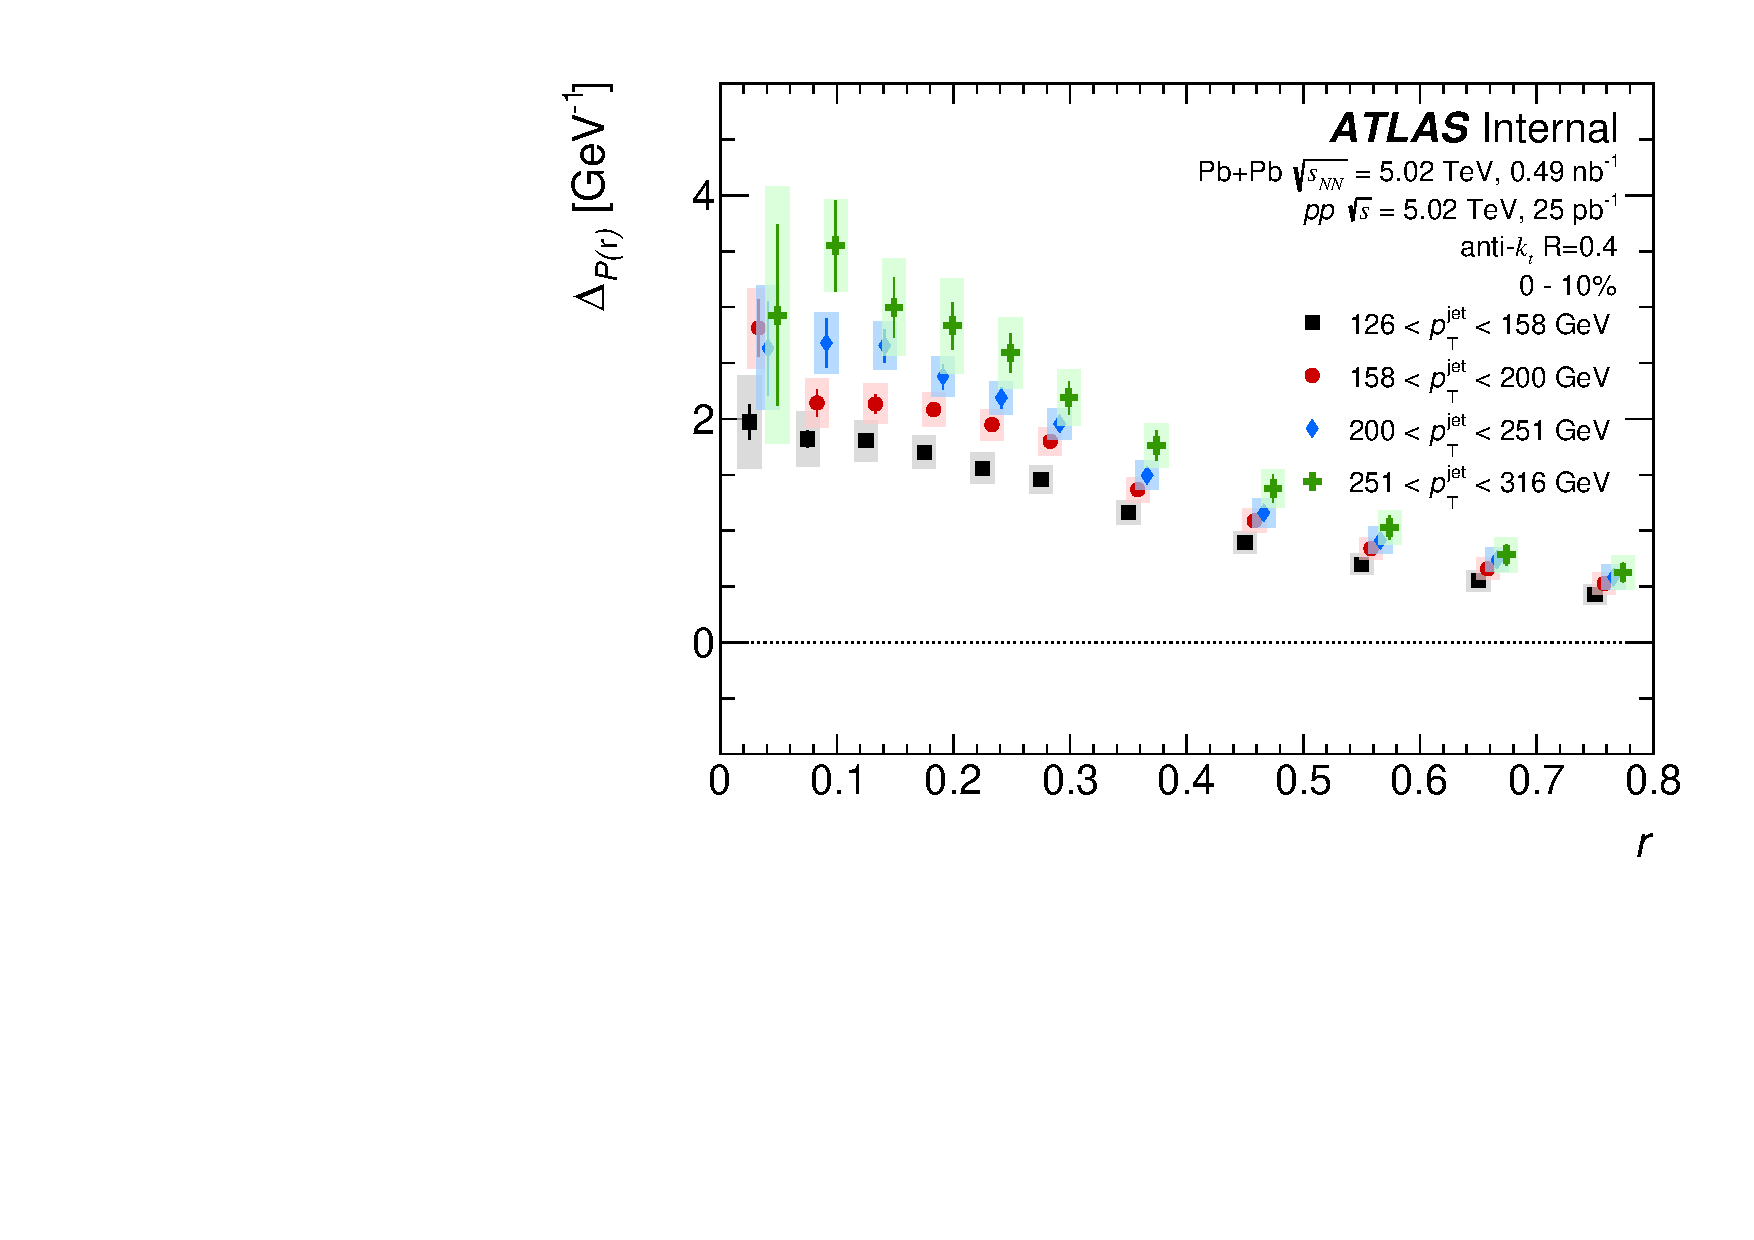
\includegraphics[width=0.5\textwidth]{results/DeltaDpT_jetshape_cent0.pdf} \\
\end{tabular} }
   \caption{\DeltaTheta\ (left) and \DeltaP\ (right) as a function of \rvar\ in central collisions for charged-particles with \pt\ < 4 GeV ranges in four \ptjet\ selections: 126--158~\GeV, 158--200~\GeV, 200--251~\GeV, and 251--316~\GeV. The vertical bars on the data points indicate statistical uncertainties while the shaded boxes indicate systematic uncertainties. The widths of the boxes are not indicative of the bin size and the points are shifted horizontally for better visibility. }
      \label{fig:deltaPdeltaT}
\end{figure}


\begin{figure}
\centering{
\begin{tabular}{cc}
	 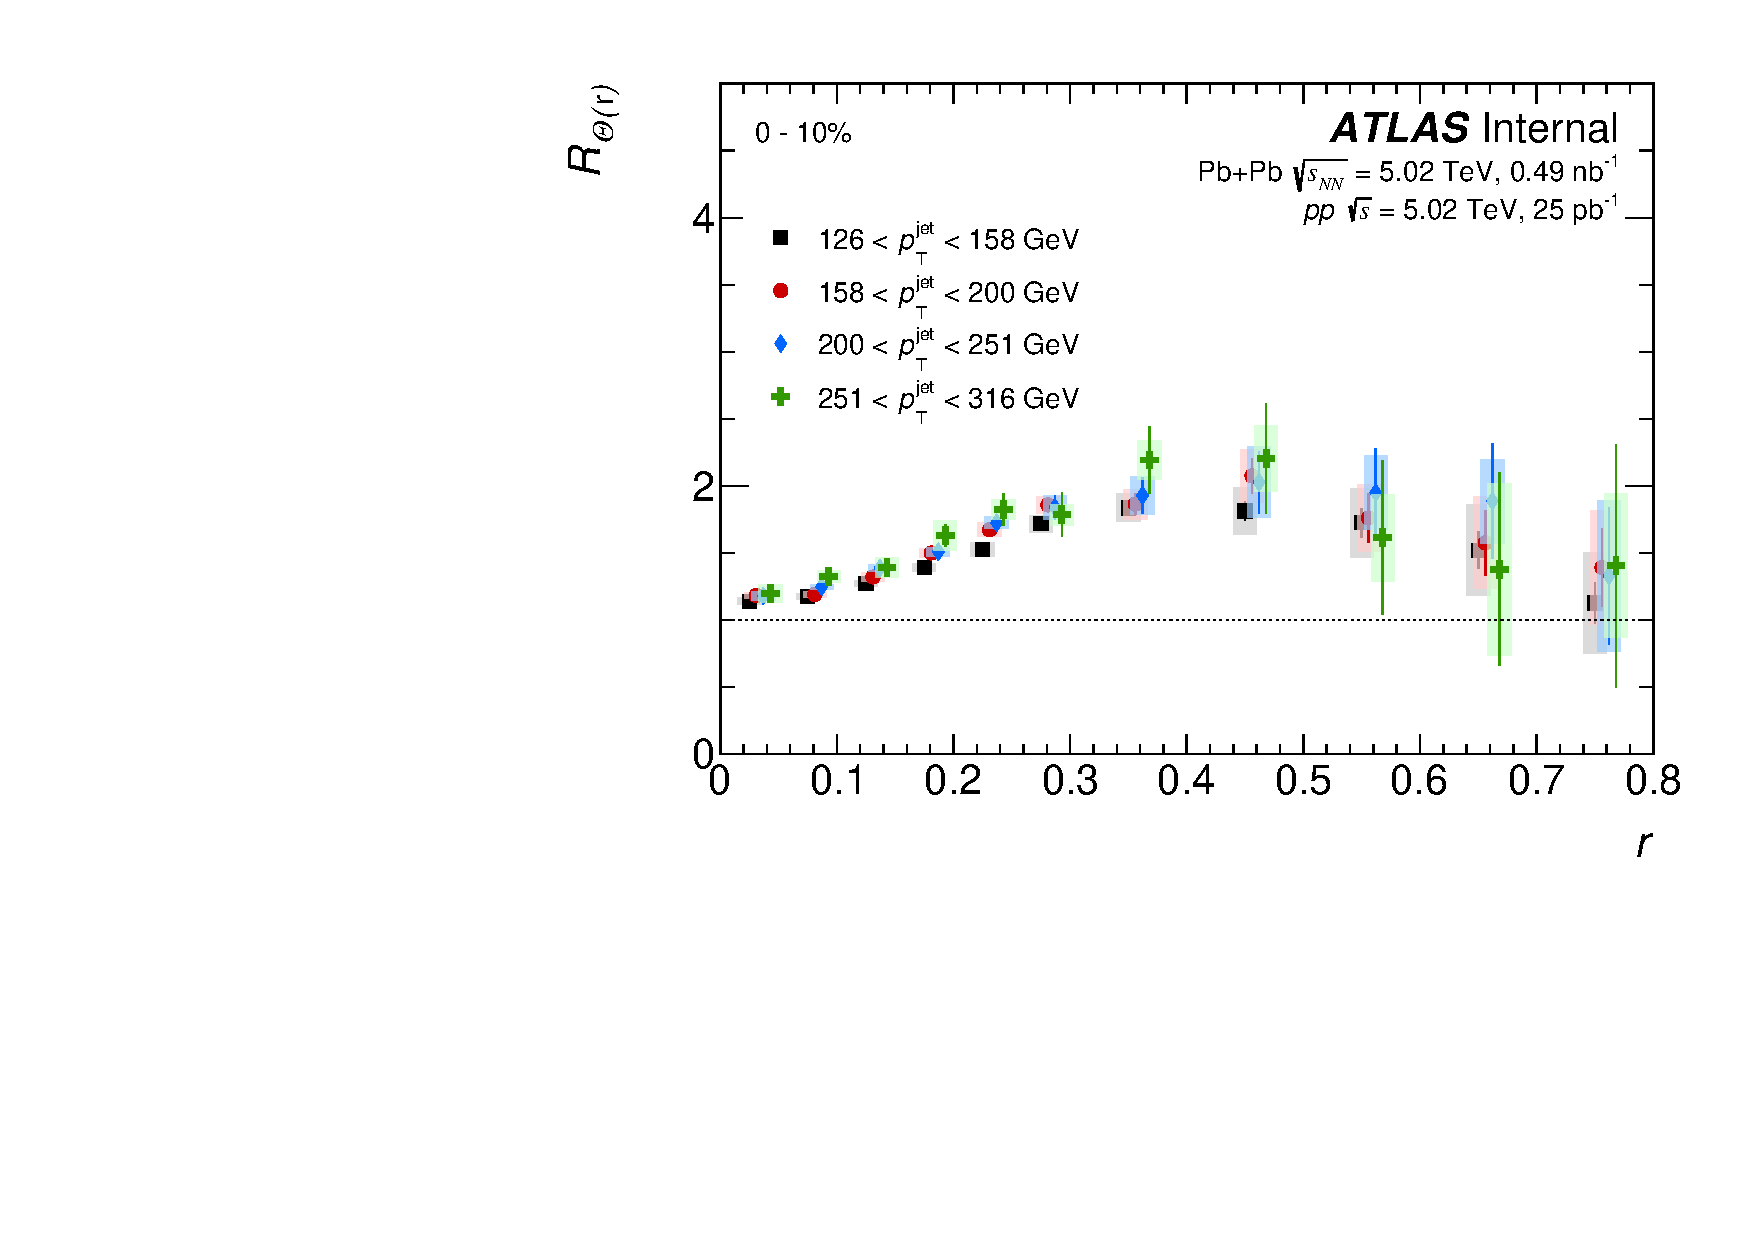
\includegraphics[width=0.5\textwidth]{results/RDpT_lowpt_integ_cent0.pdf} &
	 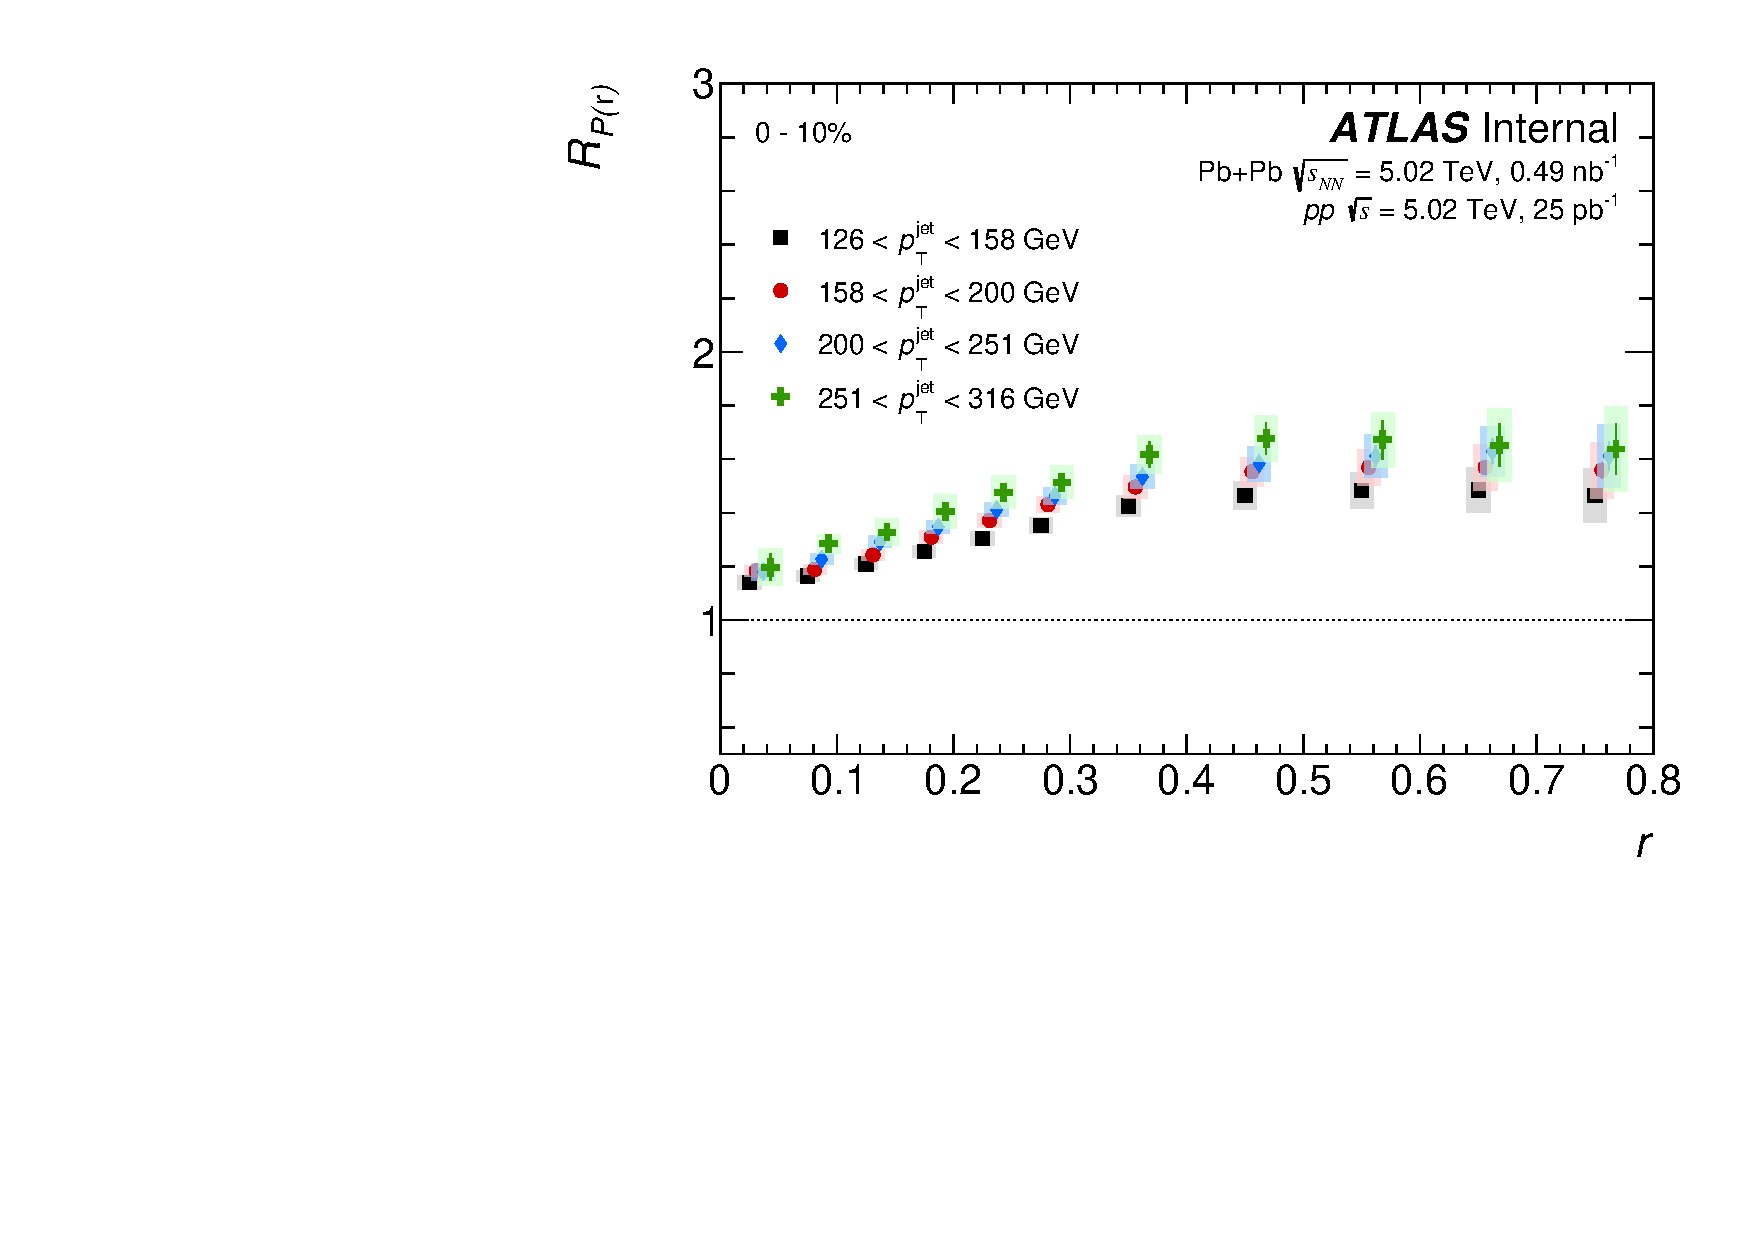
\includegraphics[width=0.5\textwidth]{results/RDpT_jetshape_cent0.pdf} \\
\end{tabular} }
   \caption{\RTheta\ (left) and \RP\ (right) as a function of \rvar\ in central collisions for charged-particles with \pt\ < 4 GeV ranges in four \ptjet\ selections: 126--158~\GeV, 158--200~\GeV, 200--251~\GeV, and 251--316~\GeV. The vertical bars on the data points indicate statistical uncertainties while the shaded boxes indicate systematic uncertainties. The widths of the boxes are not indicative of the bin size and the points are shifted horizontally for better visibility. }
      \label{fig:RPRT}
\end{figure}


%
%
%\subparagraph{Delta D jetshape: } See Figure \ref{fig:fullset_deltadptr_jetshape}
%\begin{align}
%\Delta_P = \int_0^r \int_1^{4} \Dpt_{\mathrm{PbPb}} - \Dpt_{\mathrm{pp}} \fd \pt \fd dr'
%\end{align}
%\begin{figure}[h]
%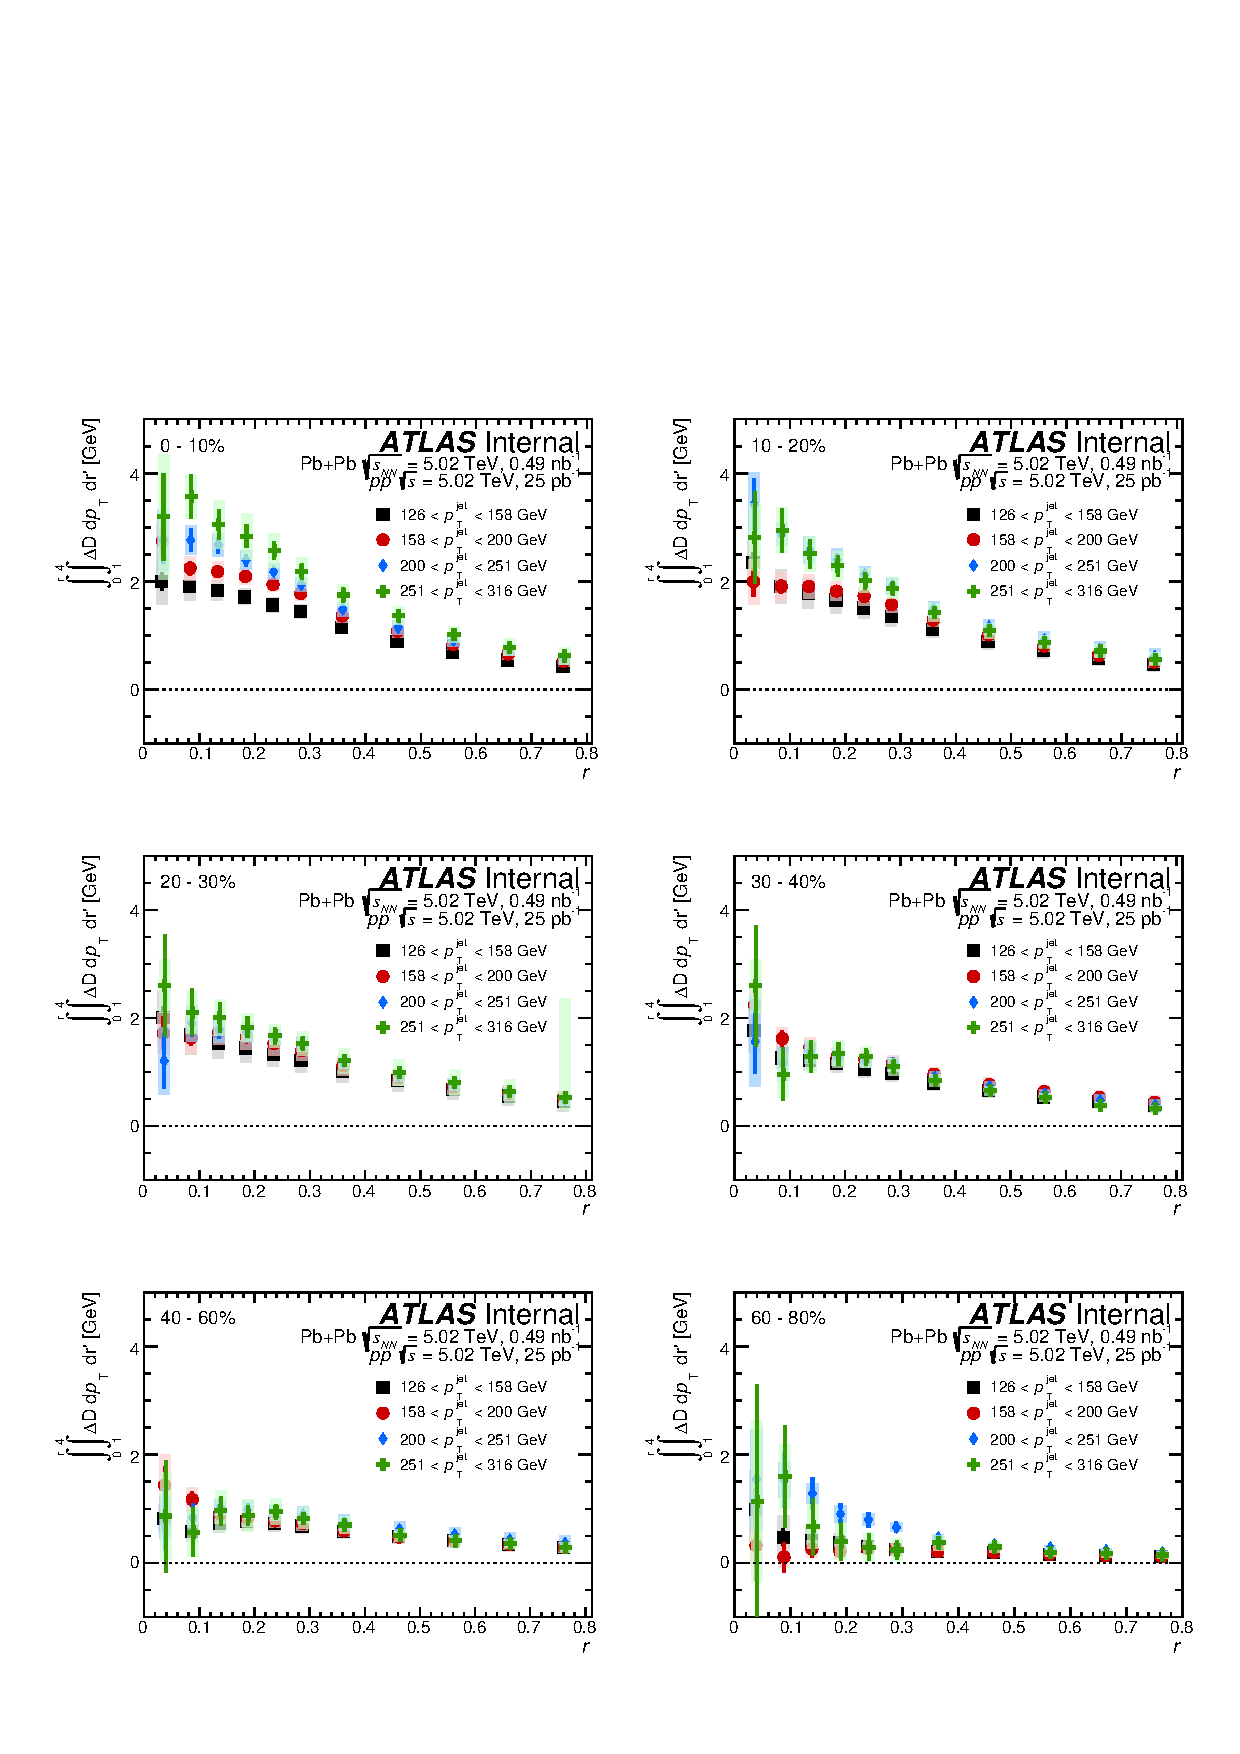
\includegraphics[width=1.0\textwidth]{figures/results/DeltaDpT_jetshape_dR.pdf}
%	\caption{Full set of \DeltaDptr\ distributions for all centralities, cumulatively integrated over r and integrated over the low \pt\ region for tracks with $ 1.0 < \pt < 4.0$ GeV. Different colors represent different \ptjet ranges}
%\label{fig:fullset_deltadptr_jetshape}
%\end{figure}
%
%
%\subparagraph{RDpT Low pT integral: } See Figure \ref{fig:fullset_rdptr_lowpT}
%\begin{align}
%R_\Theta = \frac{\int_1^{4} \Dpt_{\mathrm{PbPb}} \fd \pt }{\int_1^{4} \Dpt_{\mathrm{pp}} \fd \pt }
%\end{align}
%\begin{figure}[h]
%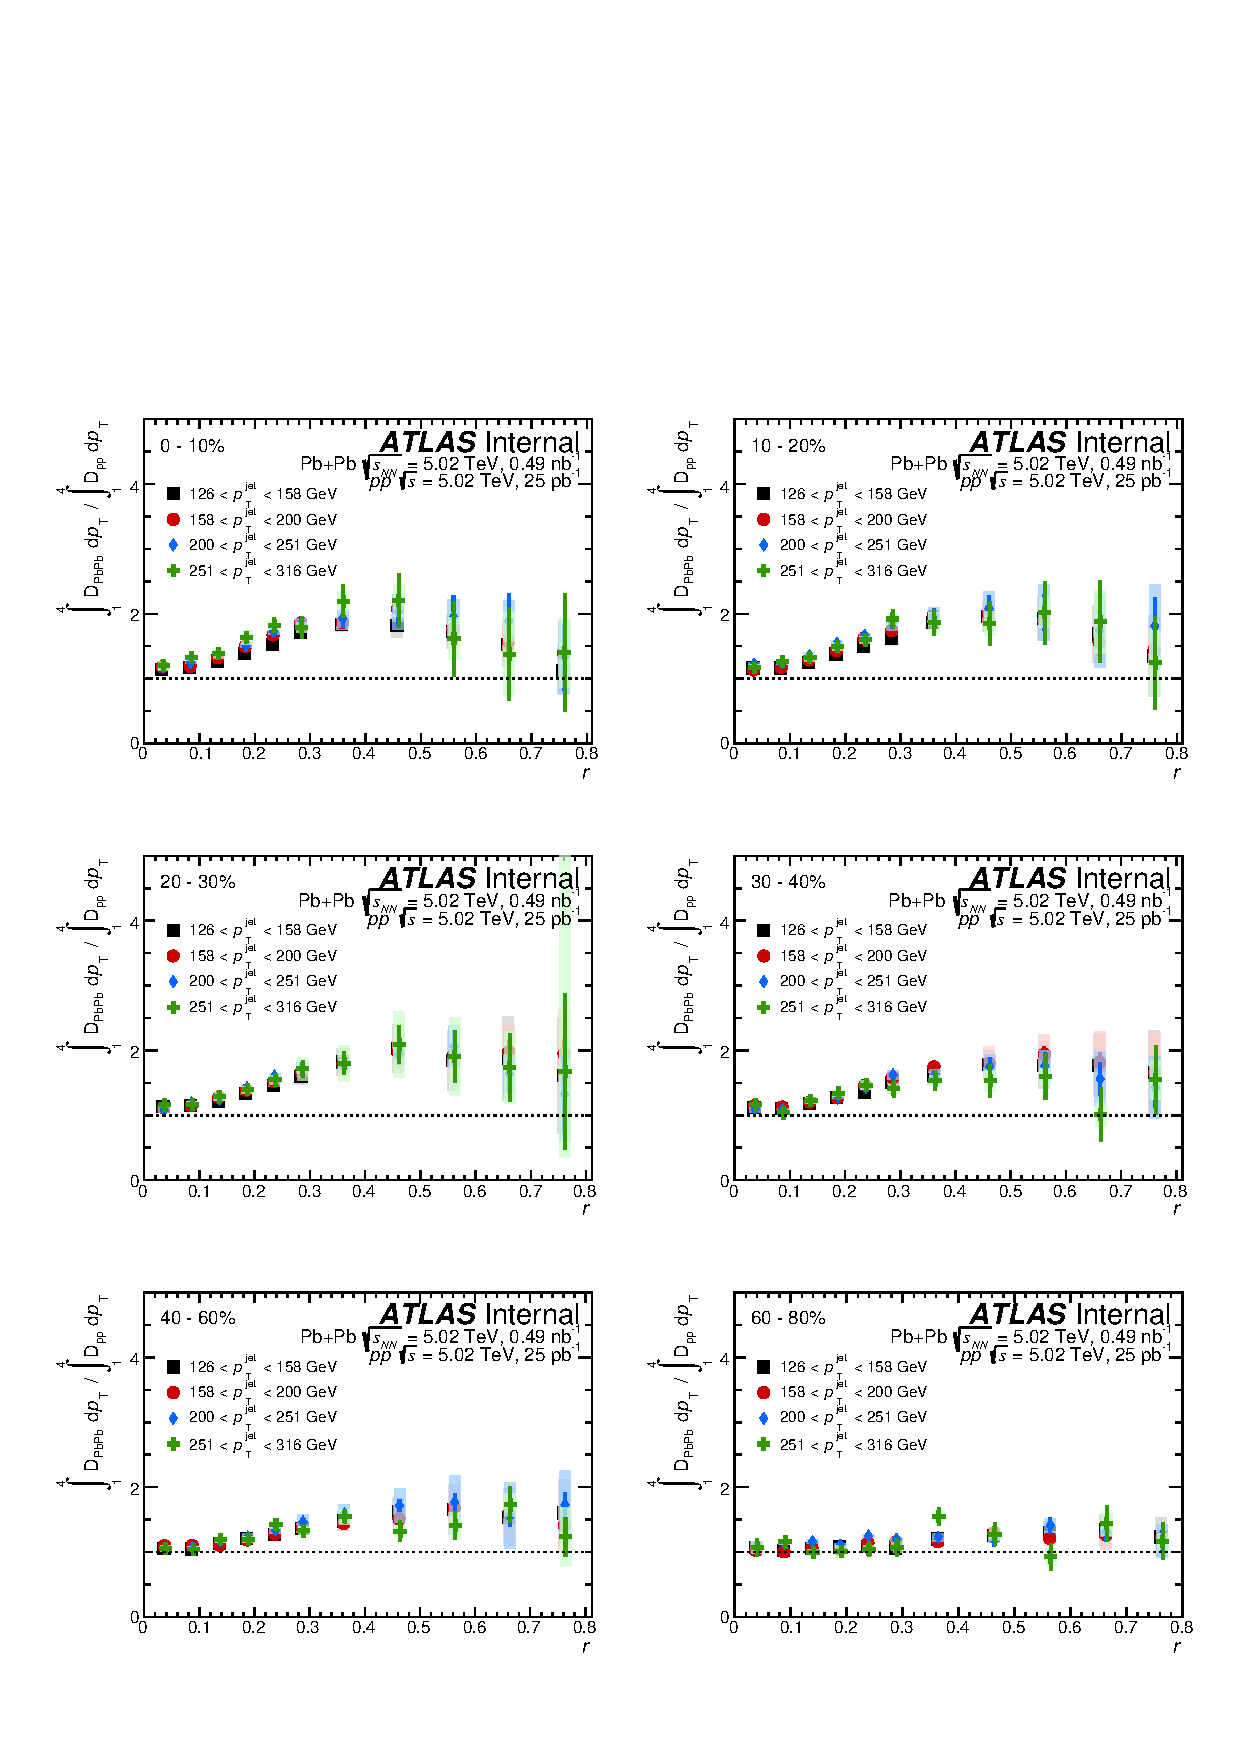
\includegraphics[width=1.0\textwidth]{figures/results/RDpT_lowpt_integ_dR.pdf}
%	\caption{Full set of \DeltaDptr\ distributions for all centralities, integrated over the low \pt\ region for tracks with $ 1.0 < \pt < 4.0$ GeV. Different colors represent different \ptjet ranges}
%\label{fig:fullset_rdptr_lowpT}
%\end{figure}
%
%
%\subparagraph{RDpT jetshape: } See Figure \ref{fig:fullset_rdptr_jetshape}
%\begin{align}
%R_P = \frac{\int_0^r \int_1^{4} \Dpt_{\mathrm{PbPb}} \fd \pt \fd r' }{\int_0^r \int_1^{4} \Dpt_{\mathrm{pp}} \fd \pt \fd r' }
%\end{align}
%\begin{figure}[h]
%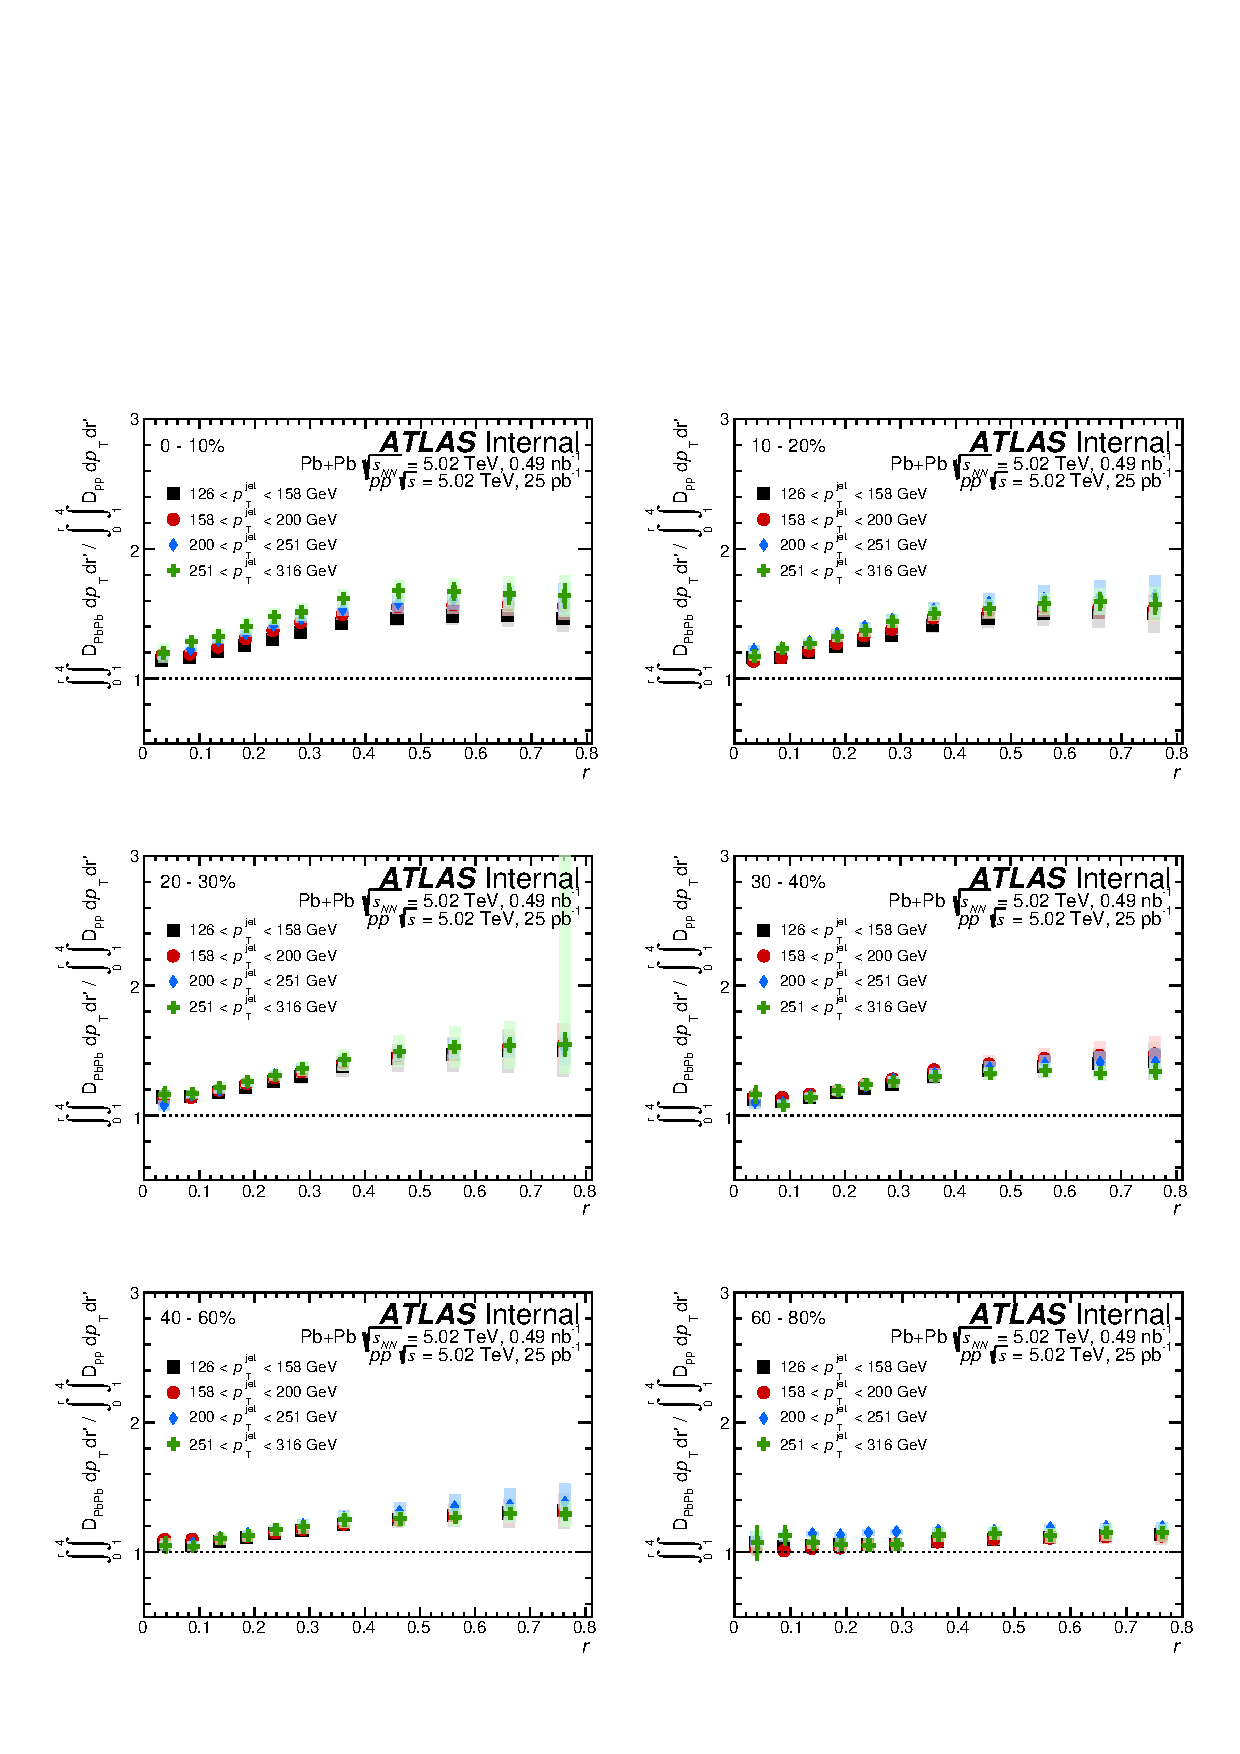
\includegraphics[width=1.0\textwidth]{figures/results/RDpT_jetshape_dR.pdf}
%	\caption{Full set of \RDptr\ distributions for all centralities, cumulatively integrated over r and integrated over the low \pt\ region for tracks with $ 1.0 < \pt < 4.0$ GeV. Different colors represent different \ptjet ranges}
%\label{fig:fullset_rdptr_jetshape}
%\end{figure}






%
% Figure~\ref{fig:fullset_deltadptr_lowpT} shows the number density of extra particles with \pt\ < 4 GeV as a function of distance from the jet axis for different \ptjet\ ranges. It can be seen that the excess increases with increasing \ptjet.
%
% Figure~\ref{fig:fullset_deltadptr_jetshape} shows the number density of extra particles with \pt\ < 4 GeV as a function of cumulative distance from the jet axis for different \ptjet\ ranges. It can be seen that at large distances from the jet axis, the overall change in low \pt\ particle density in \pbpb\ is greater by about 0.5 particles per unit area.
%
% Figure~\ref{fig:fullset_rdptr_lowpT} shows the modification between \pp\ and \pbpb\ to the number of particles with \pt\ < 4 GeV as a function of distance from the jet axis for different \ptjet\ ranges. The maximal modification near the jet edge at $0.4 < r < 0.5$ indicative of extra particles in that region that can come from large angle radiation.
%
% Figure~\ref{fig:fullset_deltadptr_lowpT} shows the modification between \pp\ and \pbpb\ to the number of particles with \pt\ < 4 GeV as a function of cumulative distance from the jet axis for different \ptjet\ ranges. There is an enhancement in the number of particles for larger cones sizes 

%
%\subparagraph{Delta D Low pT integral: } See Figure \ref{fig:fullset_deltadptr_lowpT}
%\begin{align}
%\Delta_\Theta = \int_1^{4} \Dpt_{\mathrm{PbPb}} - \Dpt_{\mathrm{pp}} \fd \pt
%\end{align}
%\begin{figure}[h]
%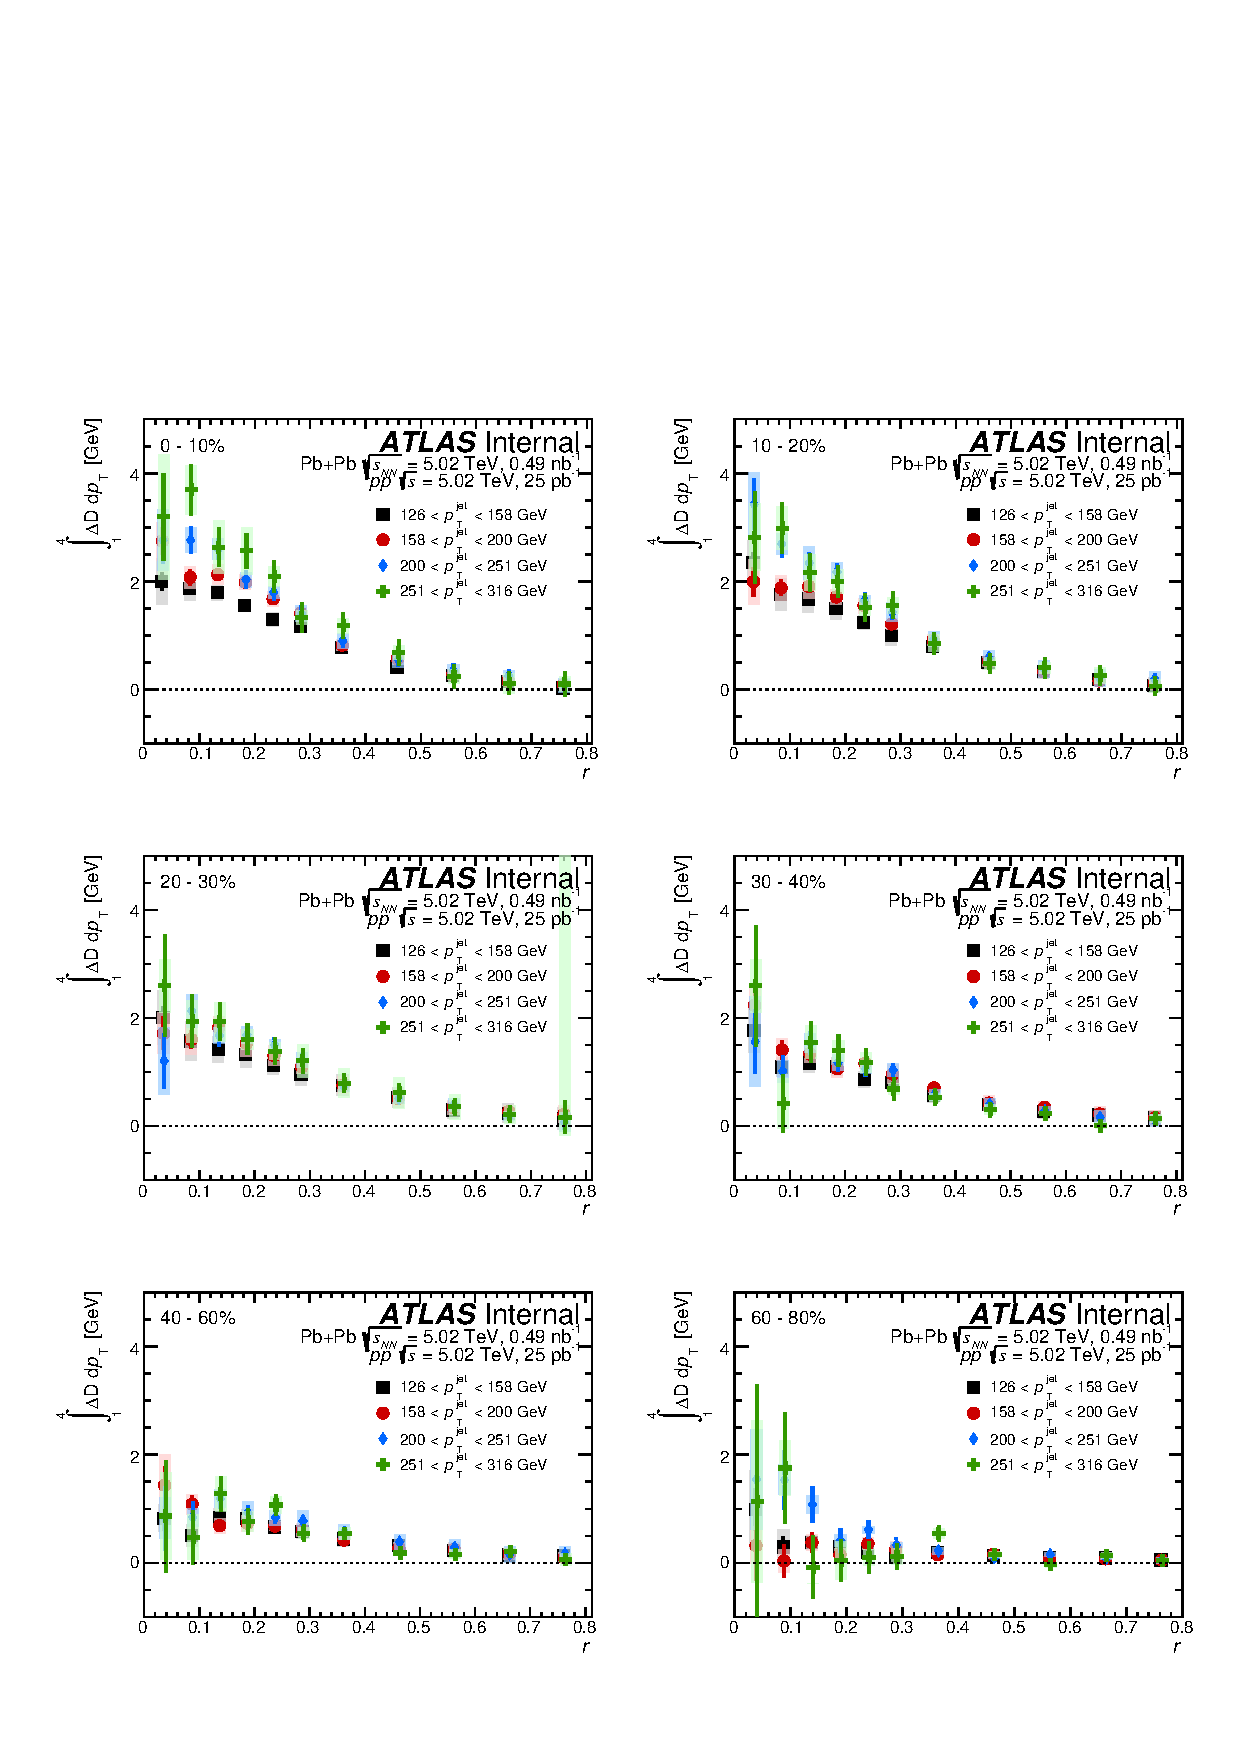
\includegraphics[width=1.0\textwidth]{figures/results/DeltaDpT_lowpt_integ_dR.pdf}
%\caption{Full set of \DeltaDptr\ distributions for all centralities, integrated over the low \pt\ region for tracks with $ 1.0 < \pt < 4.0$ GeV. Different colors represent different \ptjet ranges}
%\label{fig:fullset_deltadptr_lowpT}
%\end{figure}
%
%
%
%\subparagraph{Delta D jetshape: } See Figure \ref{fig:fullset_deltadptr_jetshape}
%\begin{align}
%\Delta_P = \int_0^r \int_1^{4} \Dpt_{\mathrm{PbPb}} - \Dpt_{\mathrm{pp}} \fd \pt \fd dr'
%\end{align}
%\begin{figure}[h]
%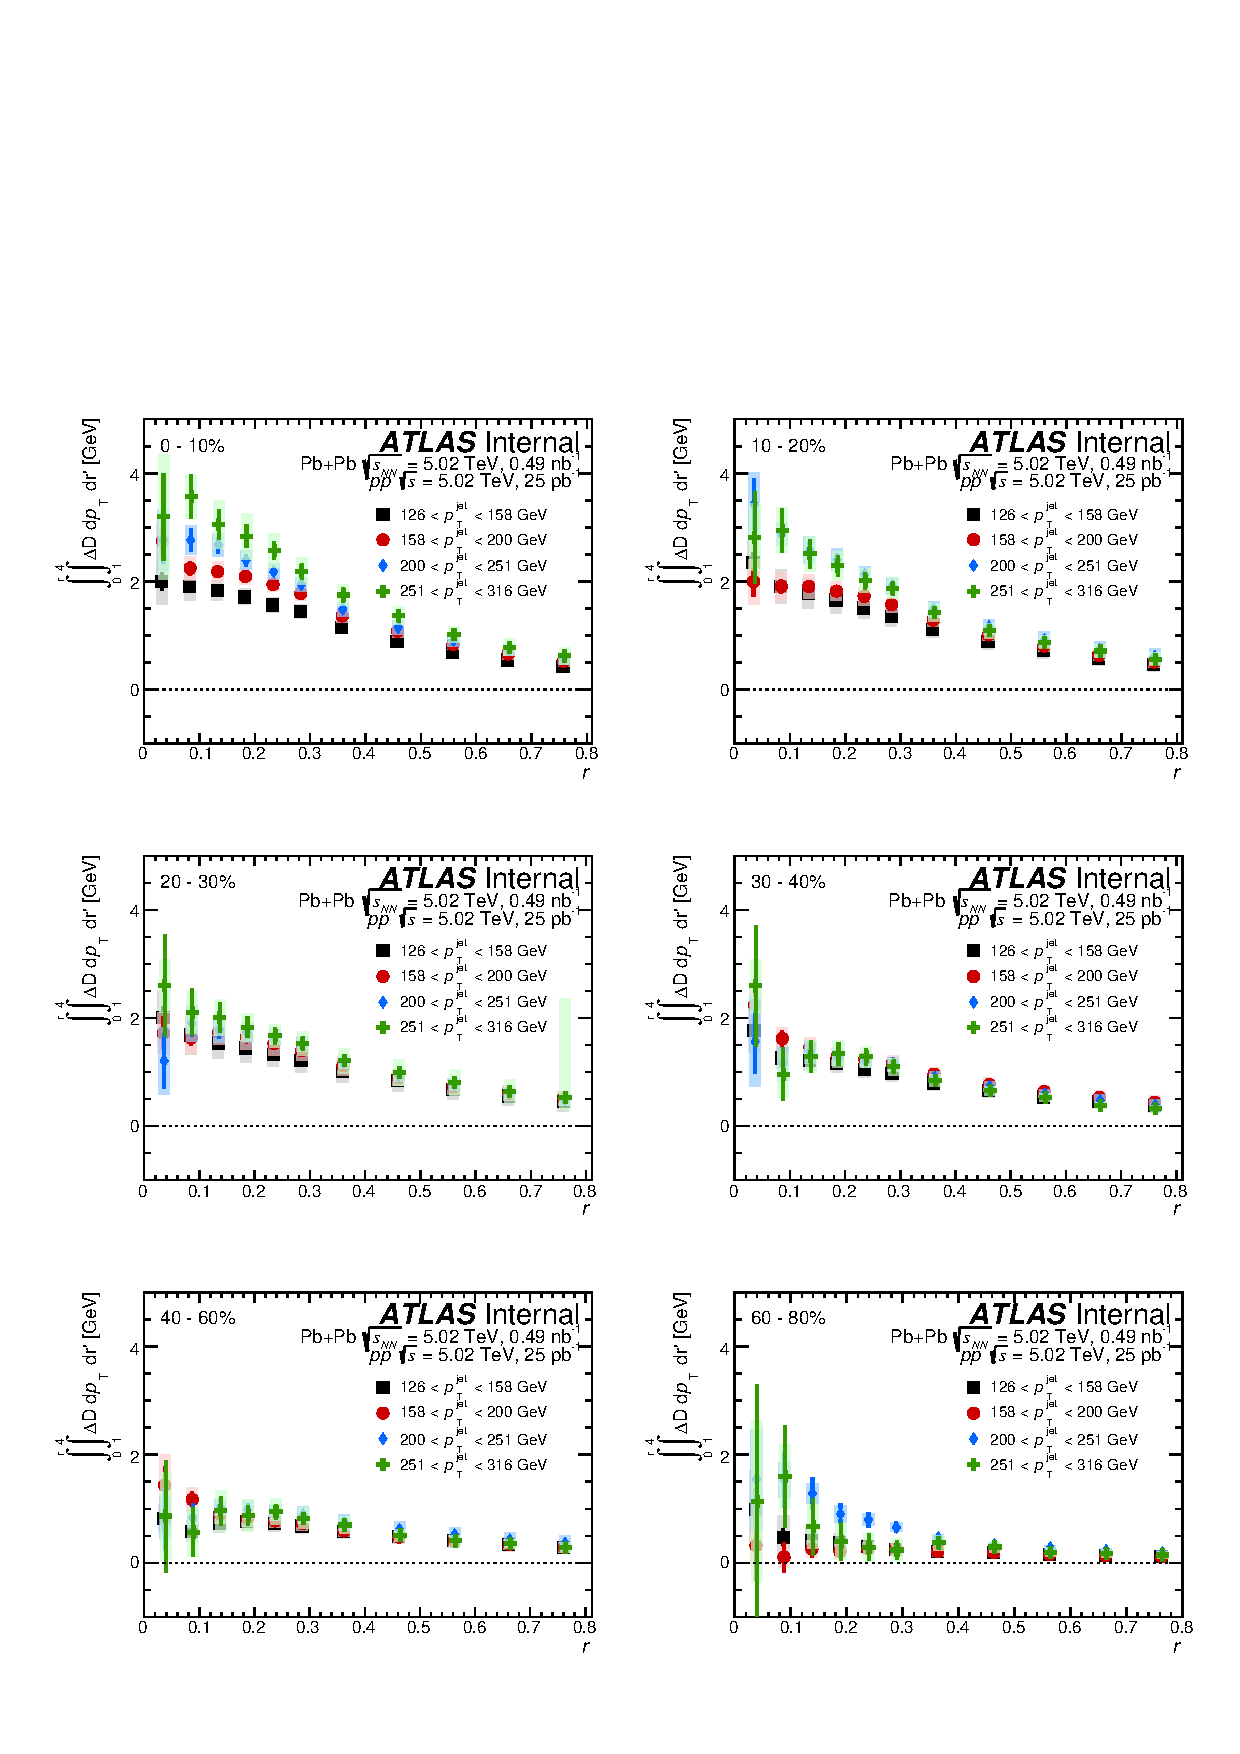
\includegraphics[width=1.0\textwidth]{figures/results/DeltaDpT_jetshape_dR.pdf}
%	\caption{Full set of \DeltaDptr\ distributions for all centralities, cumulatively integrated over r and integrated over the low \pt\ region for tracks with $ 1.0 < \pt < 4.0$ GeV. Different colors represent different \ptjet ranges}
%\label{fig:fullset_deltadptr_jetshape}
%\end{figure}
%
%
%\subparagraph{RDpT Low pT integral: } See Figure \ref{fig:fullset_rdptr_lowpT}
%\begin{align}
%R_\Theta = \frac{\int_1^{4} \Dpt_{\mathrm{PbPb}} \fd \pt }{\int_1^{4} \Dpt_{\mathrm{pp}} \fd \pt }
%\end{align}
%\begin{figure}[h]
%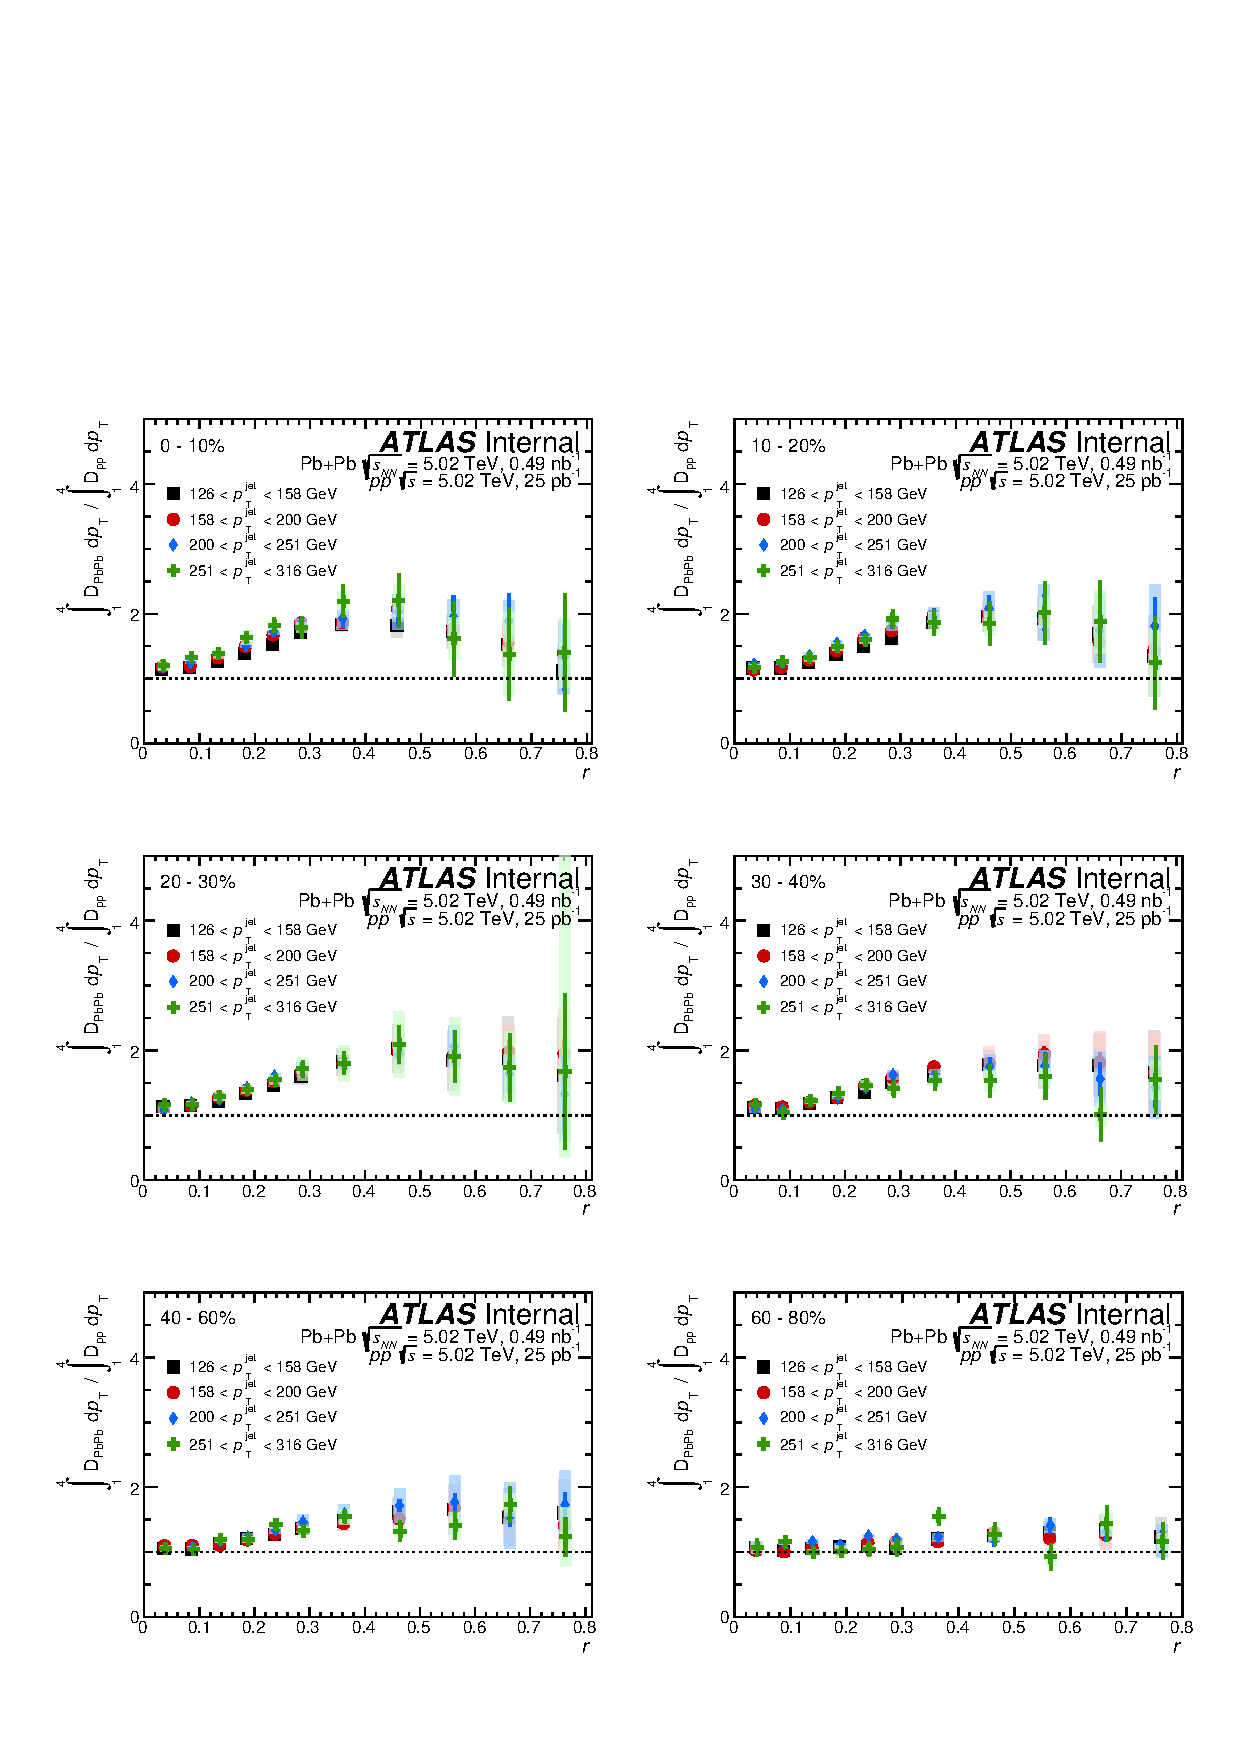
\includegraphics[width=1.0\textwidth]{figures/results/RDpT_lowpt_integ_dR.pdf}
%	\caption{Full set of \DeltaDptr\ distributions for all centralities, integrated over the low \pt\ region for tracks with $ 1.0 < \pt < 4.0$ GeV. Different colors represent different \ptjet ranges}
%\label{fig:fullset_rdptr_lowpT}
%\end{figure}
%
%
%\subparagraph{RDpT jetshape: } See Figure \ref{fig:fullset_rdptr_jetshape}
%\begin{align}
%R_P = \frac{\int_0^r \int_1^{4} \Dpt_{\mathrm{PbPb}} \fd \pt \fd r' }{\int_0^r \int_1^{4} \Dpt_{\mathrm{pp}} \fd \pt \fd r' }
%\end{align}
%\begin{figure}[h]
%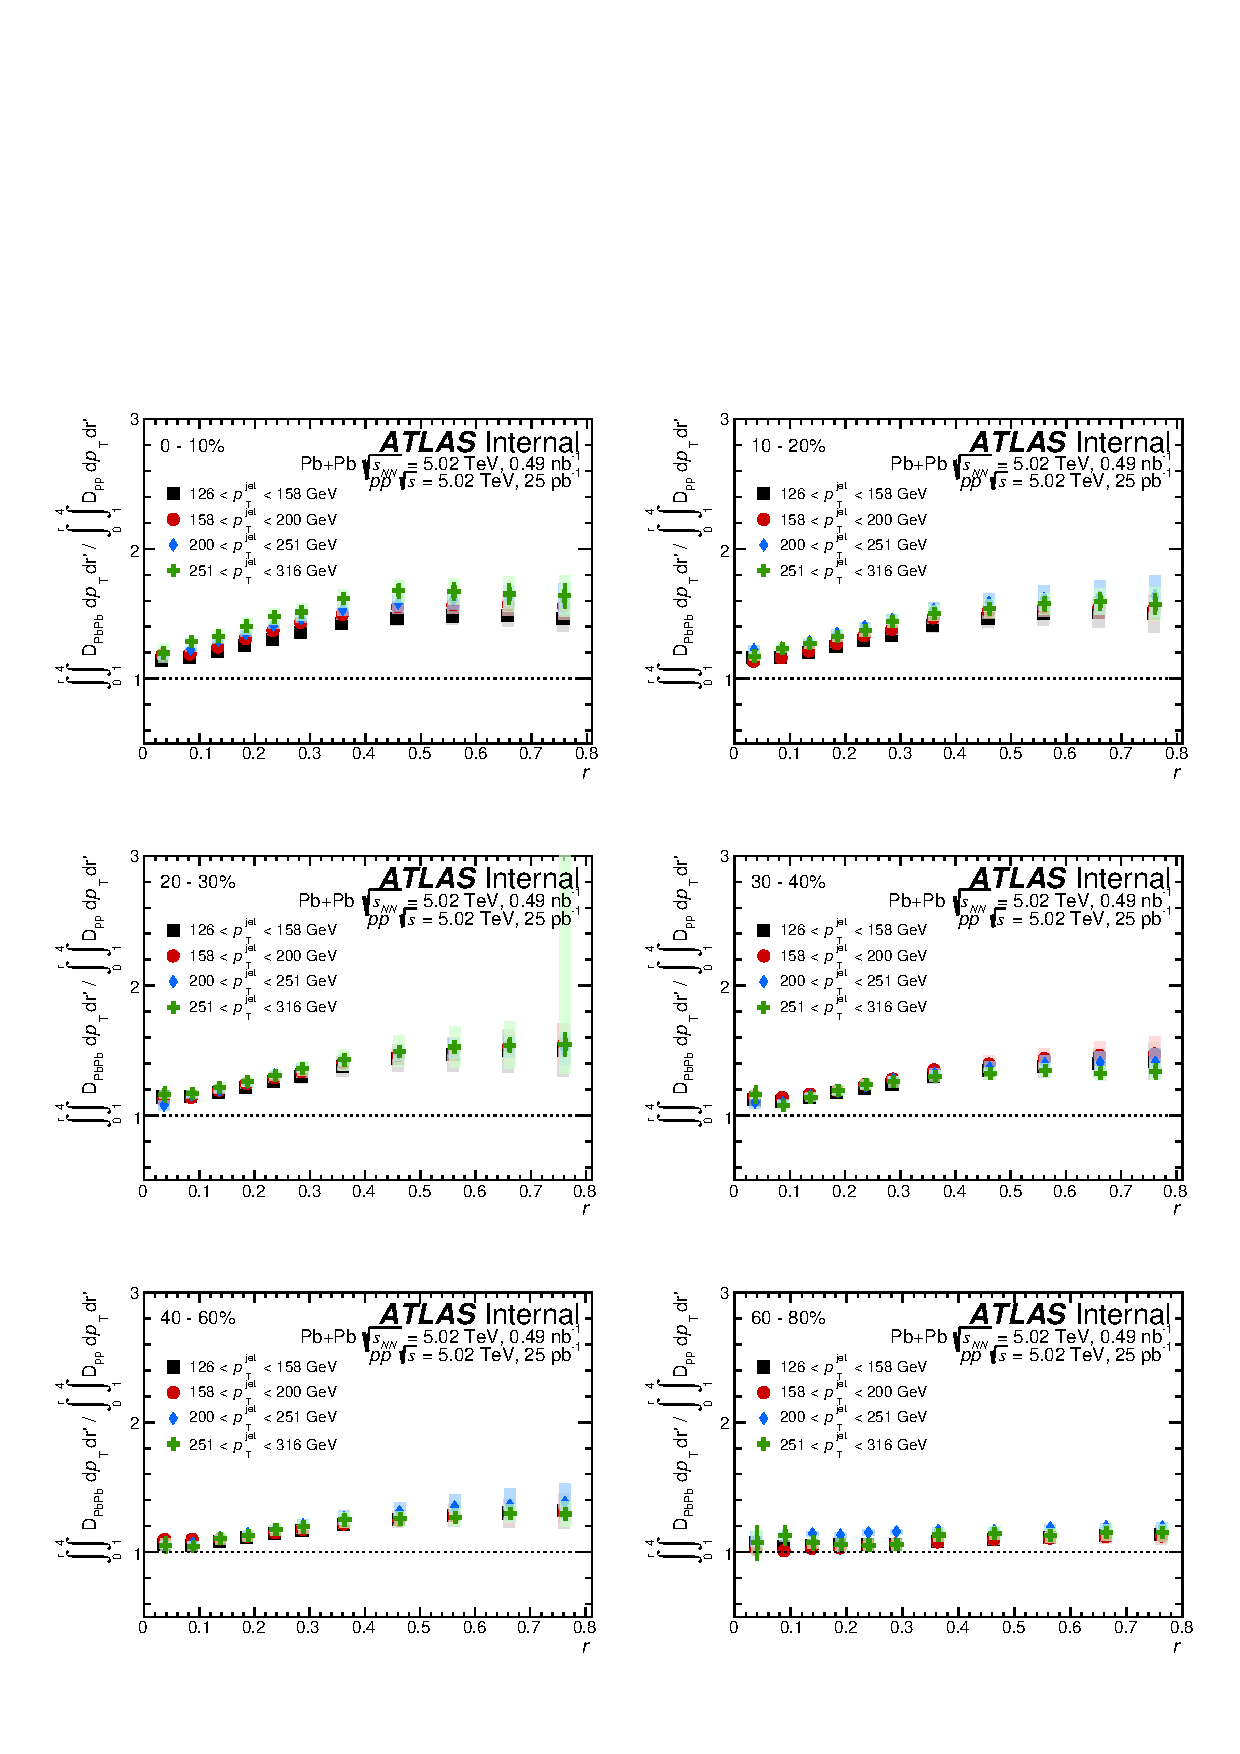
\includegraphics[width=1.0\textwidth]{figures/results/RDpT_jetshape_dR.pdf}
%	\caption{Full set of \RDptr\ distributions for all centralities, cumulatively integrated over r and integrated over the low \pt\ region for tracks with $ 1.0 < \pt < 4.0$ GeV. Different colors represent different \ptjet ranges}
%\label{fig:fullset_rdptr_jetshape}
%\end{figure}
%
%


%Delta D Low pT integral
%\begin{align}
%\int_1^{4} \Dpt_{\mathrm{PbPb}} - \Dpt_{\mathrm{pp}} \fd \pt  \\
%\int_1^{4} \Dpt_{\mathrm{PbPb}} - \Dpt_{\mathrm{pp}} \pt \fd \pt  \\
%\end{align}
%
%Delta D jetshape
%\begin{align}
%\int_0^r \int_1^{4} \Dpt_{\mathrm{PbPb}} - \Dpt_{\mathrm{pp}} \fd \pt \fd dr' \\
%\int_0^r \int_1^{4} \Dpt_{\mathrm{PbPb}} - \Dpt_{\mathrm{pp}} \pt \fd \pt \fd dr' \\
%\end{align}
%
%
%RDpT Low pT integral
%\begin{align}
%\frac{\int_1^{4} \Dpt_{\mathrm{PbPb}} \fd \pt }{\int_1^{4.2} \Dpt_{\mathrm{pp}} \fd \pt } \\
%\frac{\int_1^{4} \Dpt_{\mathrm{PbPb}} \pt \fd \pt }{\int_1^{4} \Dpt_{\mathrm{pp}} \fd \pt } \\
%\end{align}
%
%
%RDpT jetshape
%\begin{align}
%\frac{\int_0^r \int_1^{4} \Dpt_{\mathrm{PbPb}} \fd \pt \fd r' }{\int_0^r \int_1^{4.2} \Dpt_{\mathrm{pp}} \fd \pt \fd r' } \\
%\frac{\int_0^r \int_1^{4} \Dpt_{\mathrm{PbPb}} \pt \fd \pt \fd r'}{\int_0^r \int_1^{4} \Dpt_{\mathrm{pp}} \fd \pt \fd r'} \\
%\end{align}





%
%%% RDpT as function of jet pT
%\begin{figure}
%\centering{
%\begin{tabular}{cc}
%	 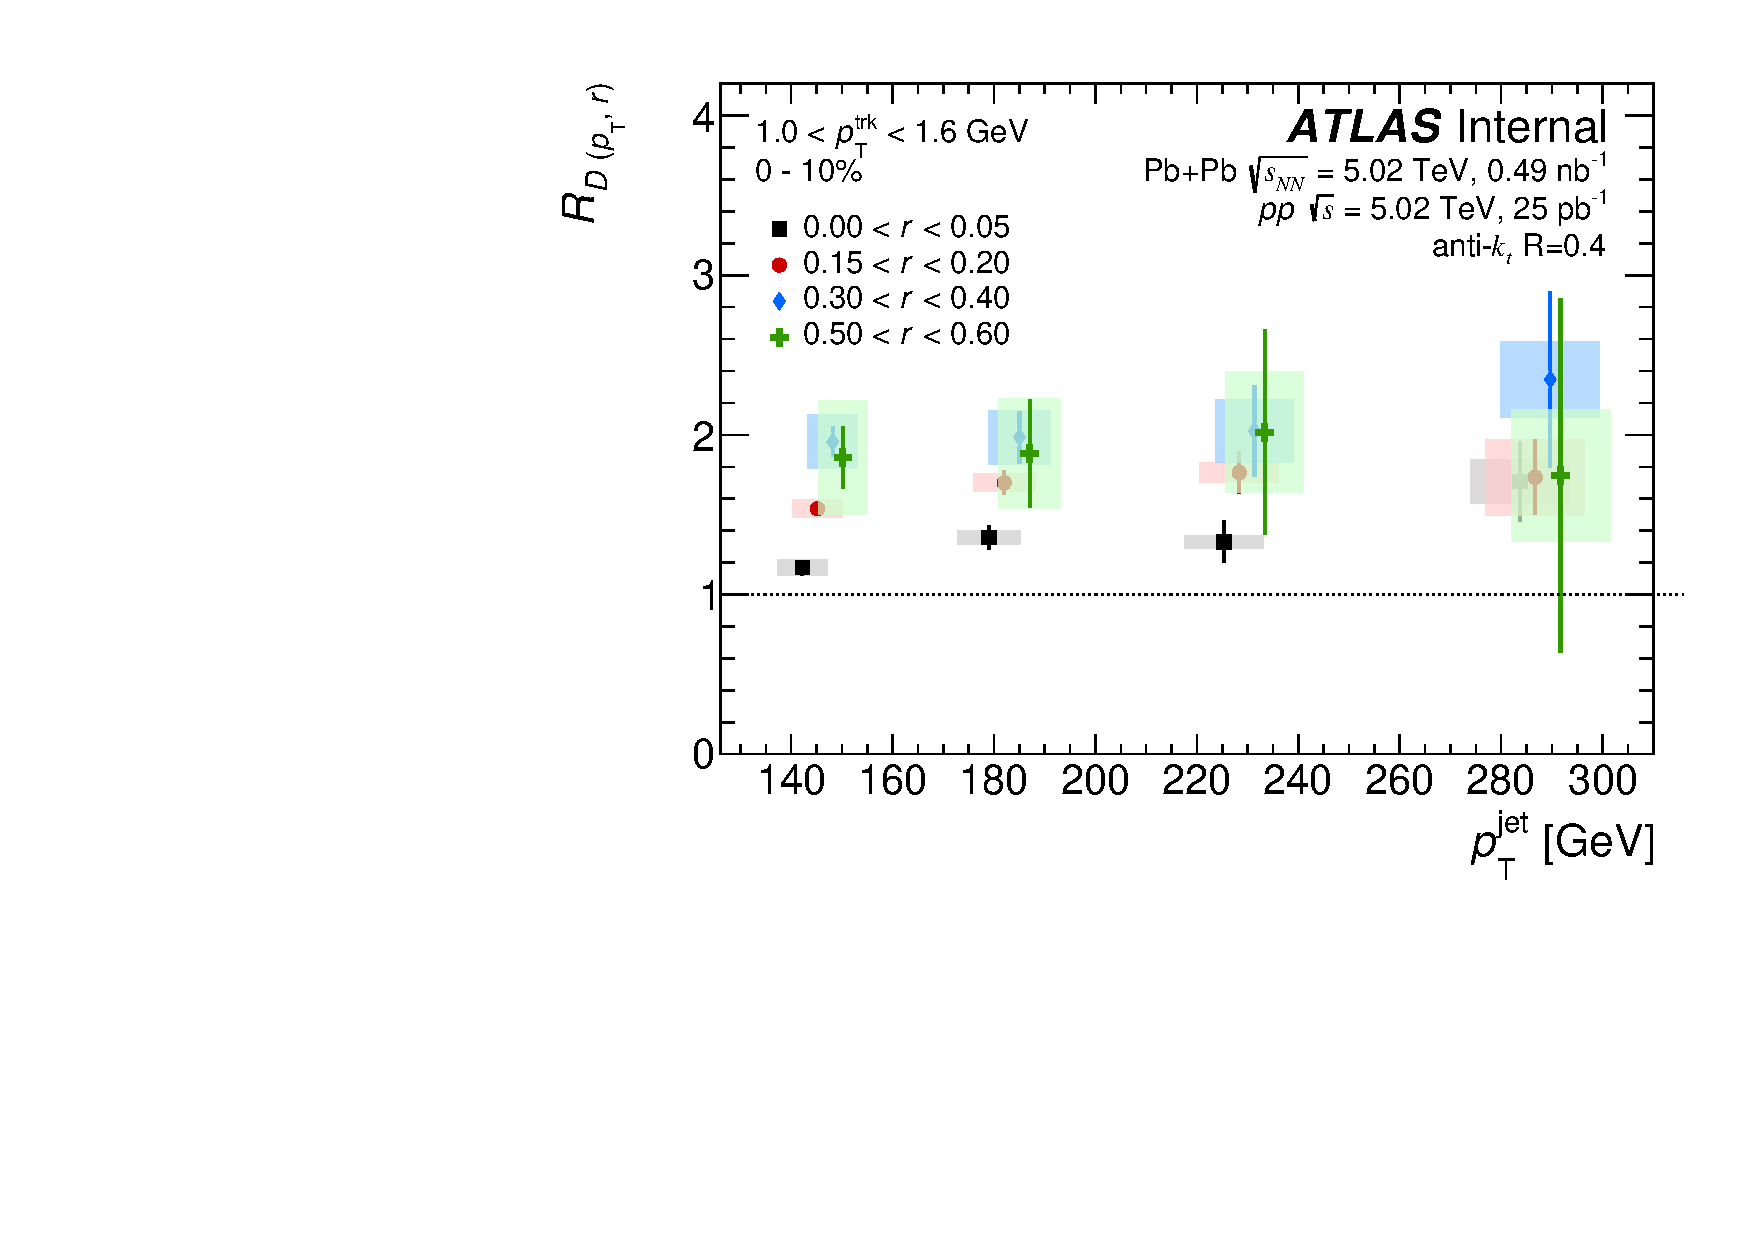
\includegraphics[width=0.45\textwidth]{results/RDpT_jetpt_trk2_cent0} &
%	 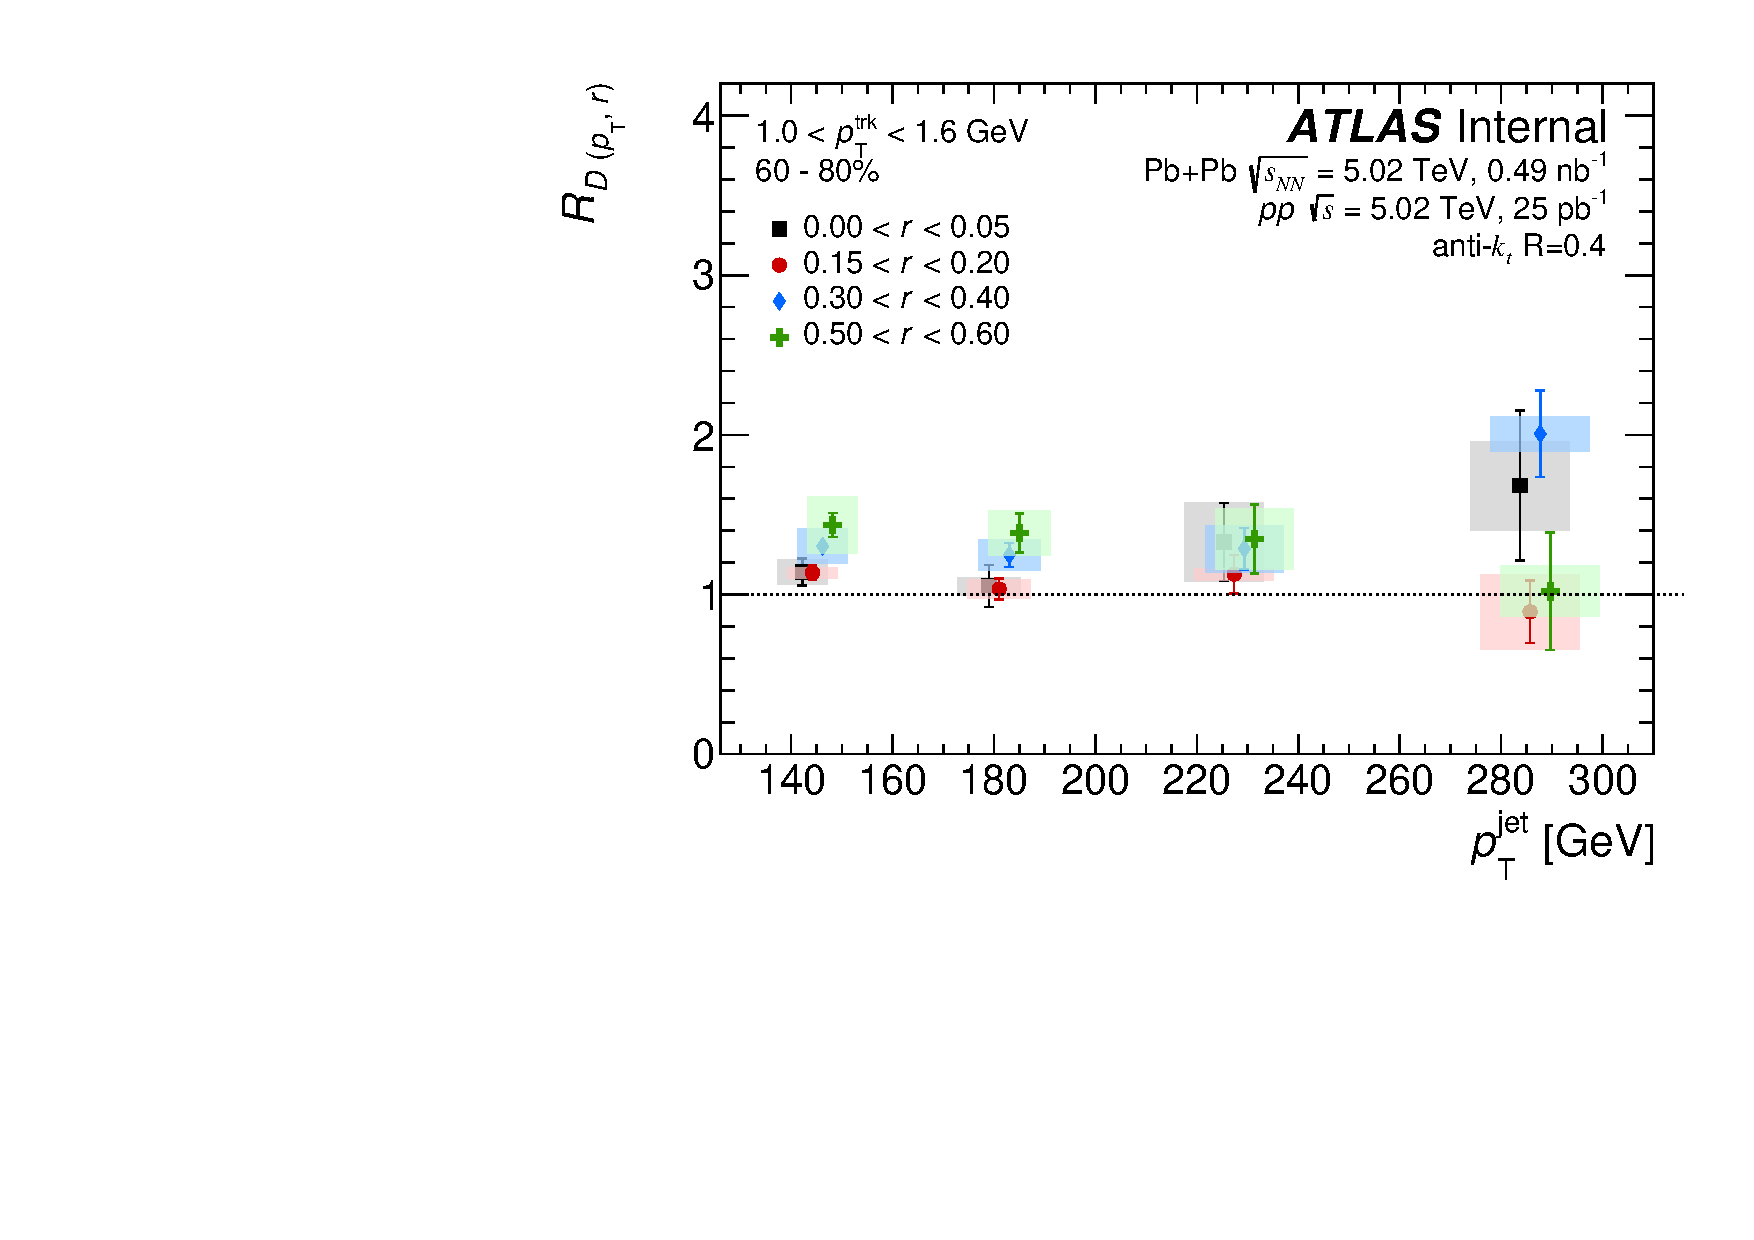
\includegraphics[width=0.45\textwidth]{results/RDpT_jetpt_trk2_cent5} \\
%	 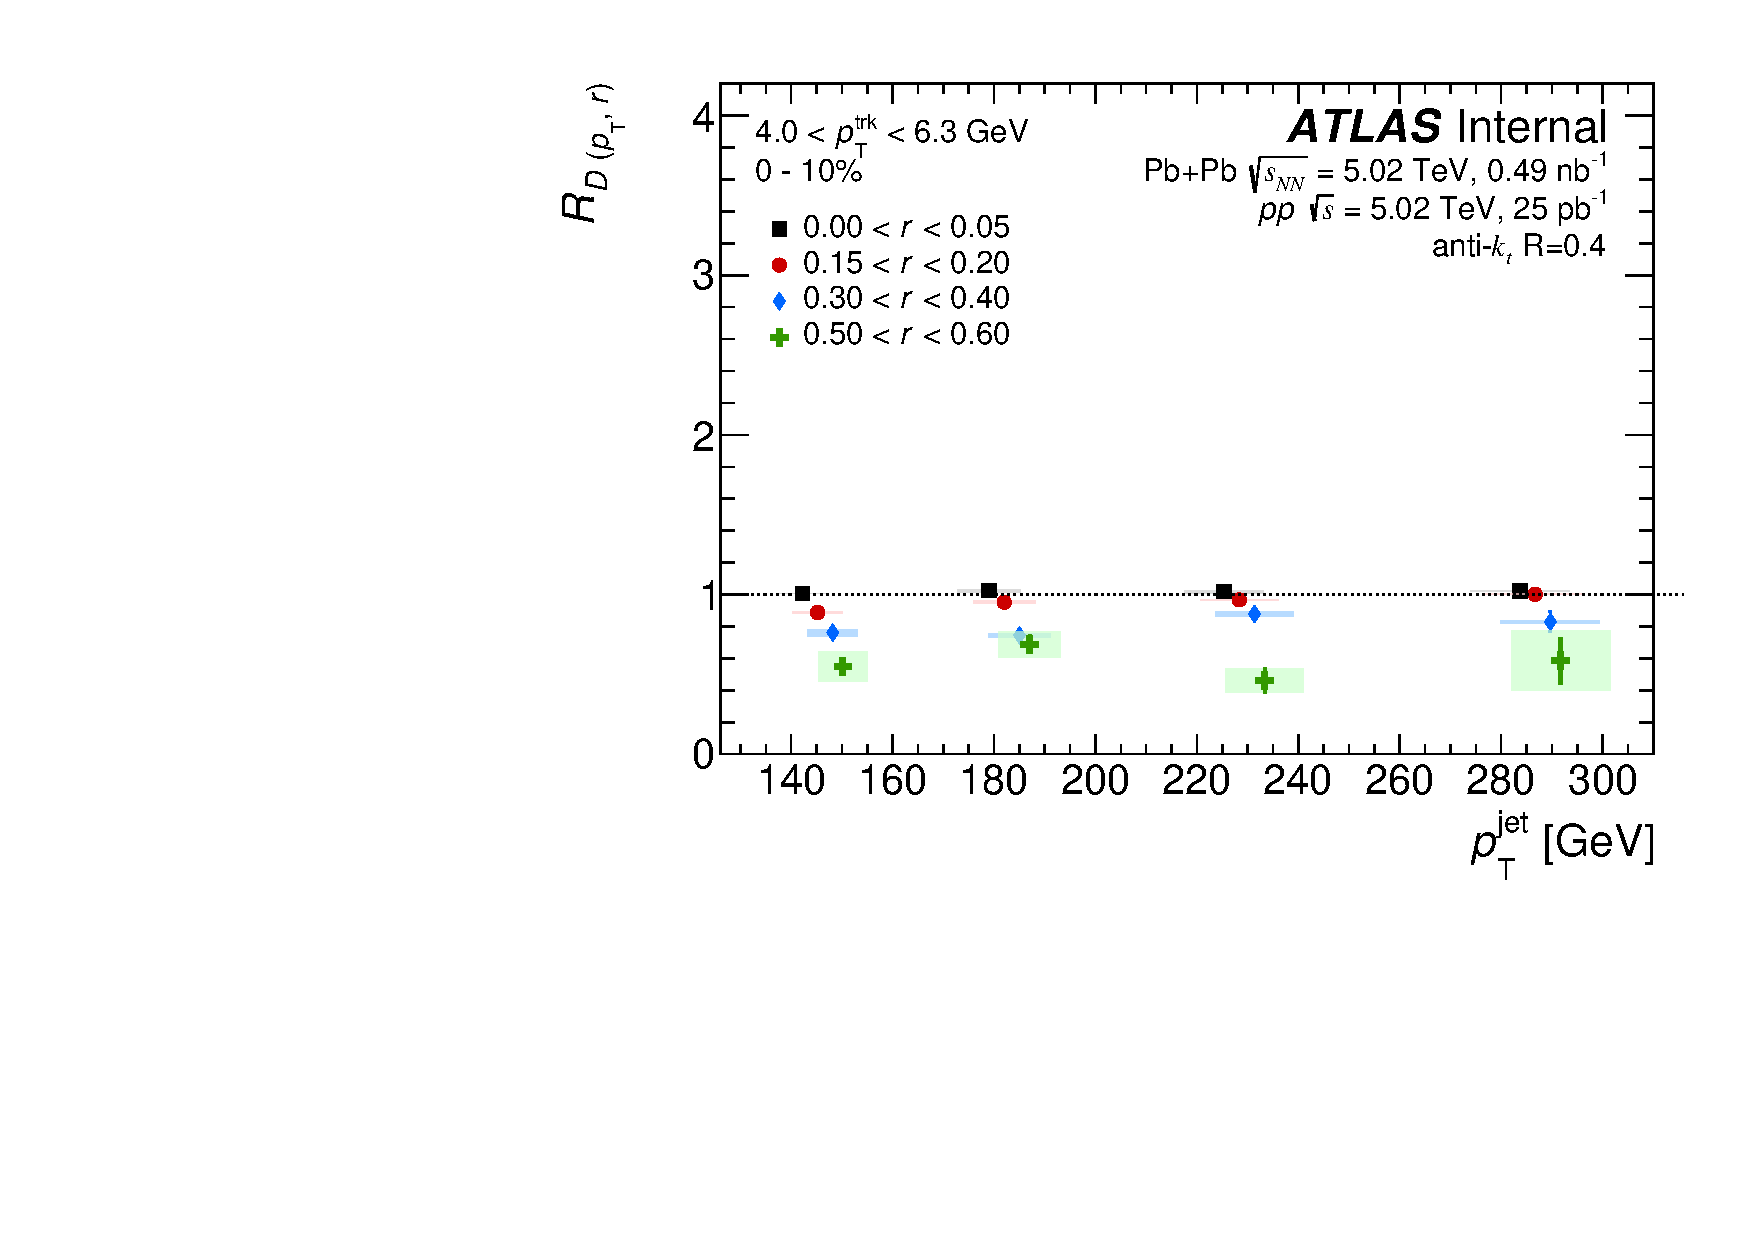
\includegraphics[width=0.45\textwidth]{results/RDpT_jetpt_trk5_cent0} &
%	 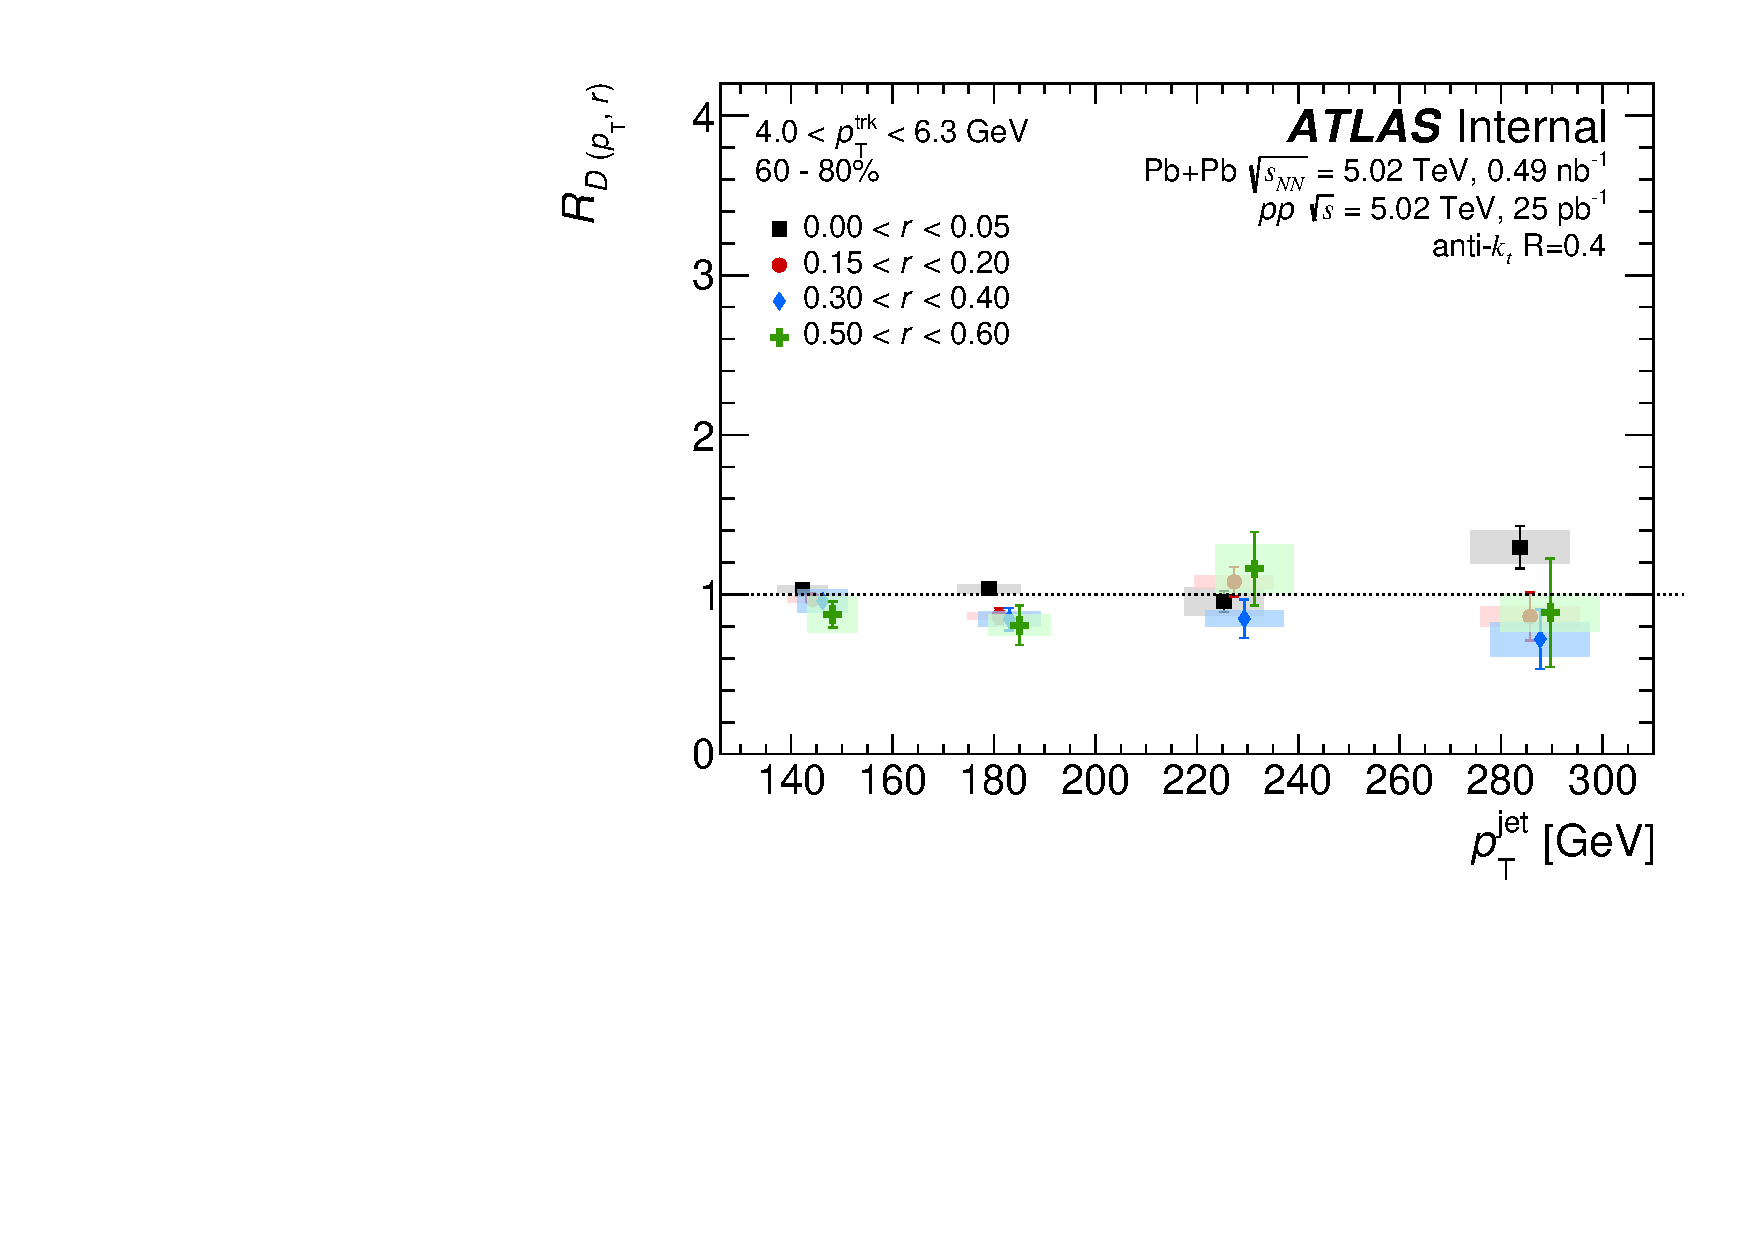
\includegraphics[width=0.45\textwidth]{results/RDpT_jetpt_trk5_cent5} \\
%\end{tabular} }
%   \caption{\RDptr as a function of \ptjet\ for charged particles with $1.0 < \pt < 1.6$ GeV (top) and $4.0 < \pt < 6.3$ GeV (bottom) at different distances from the jet axis and in 0--10\% central (left) and 60--80\% peripheral (right) \pbpb\ collisions. The vertical bars on the data points indicate statistical uncertainties while the shaded boxes indicate systematic uncertainties. The widths of the boxes are not indicative of the bin size and the points are shifted horizontally for better visibility.}
%      \label{fig:rdptr_jetpt}
%\end{figure}

%\begin{align}
%\frac{\int_1^{4} \Dpt_{\mathrm{PbPb}} \fd \pt }{\int_1^{4.2} \Dpt_{\mathrm{pp}} \fd \pt } &\qquad \frac{\int_1^{4} \Dpt_{\mathrm{PbPb}} \pt \fd \pt }{\int_1^{4} \Dpt_{\mathrm{pp}} \fd \pt } \\
%\int_1^{4} \Dpt_{\mathrm{PbPb}} - \Dpt_{\mathrm{pp}} \fd \pt  &\qquad \int_1^{4} \Dpt_{\mathrm{PbPb}} - \Dpt_{\mathrm{pp}} \pt \fd \pt \\
%\frac{\int_0^r \int_1^{4} \Dpt_{\mathrm{PbPb}} \fd \pt \fd r' }{\int_0^r \int_1^{4.2} \Dpt_{\mathrm{pp}} \fd \pt \fd r' } &\qquad \frac{\int_0^r \int_1^{4} \Dpt_{\mathrm{PbPb}} \pt \fd \pt \fd r'}{\int_0^r \int_1^{4} \Dpt_{\mathrm{pp}} \fd \pt \fd r'} \\
%\int_0^r \int_1^{4} \Dpt_{\mathrm{PbPb}} - \Dpt_{\mathrm{pp}} \fd \pt \fd dr'  &\qquad \int_0^r \int_1^{4} \Dpt_{\mathrm{PbPb}} - \Dpt_{\mathrm{pp}} \pt \fd \pt \fd dr'
%\end{align}

The measured dependence of \RDptr\ suggests that the energy lost by jets through the jet quenching process is being transferred to particles with $\pt <$~4.0~\GeV\ at larger radial distances from the jet axis. This is qualitatively consistent with theoretical calculations \mbox{\cite{Qin:2015srf,Blaizot:2014ula}}.


These observations are in agreement with the previous measurement of jet fragmentation functions \cite{Chatrchyan:2014ava, Sirunyan:2018jqr, Aaboud:2017bzv, PhysRevC.98.024908} and may indicate the dependence of the response of the hot dense matter to the momentum of a jet passing through it. 


\FloatBarrier
